\documentclass{ieeeaccess}
\usepackage{cite}
\usepackage{amsmath,amssymb,amsfonts}
\usepackage{algorithmic}
\usepackage{graphicx}
\usepackage{textcomp}
\usepackage{multirow}
\extrafloats{100}

\usepackage{bm}
\makeatletter
\AtBeginDocument{\DeclareMathVersion{bold}
\SetSymbolFont{operators}{bold}{T1}{times}{b}{n}
\SetSymbolFont{NewLetters}{bold}{T1}{times}{b}{it}
\SetMathAlphabet{\mathrm}{bold}{T1}{times}{b}{n}
\SetMathAlphabet{\mathit}{bold}{T1}{times}{b}{it}
\SetMathAlphabet{\mathbf}{bold}{T1}{times}{b}{n}
\SetMathAlphabet{\mathtt}{bold}{OT1}{pcr}{b}{n}
\SetSymbolFont{symbols}{bold}{OMS}{cmsy}{b}{n}
\renewcommand\boldmath{\@nomath\boldmath\mathversion{bold}}}
\makeatother

\def\BibTeX{{\rm B\kern-.05em{\sc i\kern-.025em b}\kern-.08em
    T\kern-.1667em\lower.7ex\hbox{E}\kern-.125emX}}

%Your document starts from here ___________________________________________________
\begin{document}
\history{Date of publication xxxx 00, 0000, date of current version xxxx 00, 0000.}
\doi{10.1109/ACCESS.2024.0429000}

\title{Development of Quantum Kernel in Quantum Machine Learning for Green Tea Grade Classification}
\author{\uppercase{First A. Author}\authorrefmark{1}, \IEEEmembership{Fellow, IEEE},
\uppercase{Second B. Author}\authorrefmark{2}, and Third C. Author,
Jr.\authorrefmark{3},
\IEEEmembership{Member, IEEE}}

\address[1]{National Institute of Standards and
Technology, Boulder, CO 80305 USA (e-mail: author@boulder.nist.gov)}
\address[2]{Department of Physics, Colorado State University, Fort Collins,
CO 80523 USA (e-mail: author@lamar.colostate.edu)}
\address[3]{Electrical Engineering Department, University of Colorado, Boulder, CO
80309 USA}
\tfootnote{This paragraph of the first footnote will contain support
information, including sponsor and financial support acknowledgment. For
example, ``This work was supported in part by the U.S. Department of
Commerce under Grant BS123456.''}

\markboth
{Author \headeretal: Preparation of Papers for IEEE TRANSACTIONS and JOURNALS}
{Author \headeretal: Preparation of Papers for IEEE TRANSACTIONS and JOURNALS}

\corresp{Corresponding author: First A. Author (e-mail: author@ boulder.nist.gov).}


\begin{abstract}
Organoleptic evaluation of the quality of green tea is traditionally subjective, costly, and time consuming. To address these limitations, Electronic Nose (E-nose) technology offers an objective alternative; however, its application to dry (non-infused) tea samples faces challenges due to weak aroma intensity and overlapping data patterns, which hinder accurate classification by classical algorithms such as Support Vector Machine (SVM). This study aims to develop a Quantum Machine Learning (QML) model using a Quantum Support Vector Machine (QSVM) for multiclass classification across five green tea grades, namely grades A, B, C, D, and E. The approach employs Quantum Kernel Estimation (QKE) with Instantaneous Quantum Polynomial (IQP) circuits, exploring different entanglement topologies (full, linear, circular) and Pauli-based kernels to embed the data into a high-dimensional Hilbert space. To maximize model performance, hyperparameter optimization is performed using Grid Search. The study seeks to demonstrate that quantum kernels can achieve higher accuracy than classical kernels when handling noisy, overlapping data in tea quality classification.
\end{abstract}

\begin{keywords}
Instantaneous Quantum Polynomial, Pauli, Quantum Kernel Estimation, Quantum Machine Learning, Quantum Support Vector Machine
\end{keywords}

\titlepgskip=-21pt

\maketitle

\section{Introduction}

\section{Related Works}

\section{Methodology}
\label{sec:methodology}

This section describes the dataset and its grouped structure, the group-aware cross-validation that prevents data leakage, the shared preprocessing pipeline, the evaluation metrics and the minority-aware Composite selection score, the classical and deep learning baselines, the quantum kernel models including the proposed STAR-v2 feature map, and the hyperparameter optimization protocol.

\subsection{Dataset and Class Structure}
\label{subsec:dataset}

The experiments use an electronic-nose (e-nose) dataset of dry, non-infused green tea. Each measurement is a vector of twelve features, comprising ten metal-oxide gas-sensor responses, humidity, and temperature recorded during acquisition. Every sample is labeled with one of five quality grades, A, B, C, D, and E, as assigned by professional tea testers. The dataset contains 10{,}409 rows.

The dataset is collected using hierarchical approach, which represent 69 physical tea samples identified by Chop\_ID and collected across 274 acquisition sessions, which identified by Sampling\_ID, since each physical sample is recorded around forty consecutive time-steps of the sensor array. The dataset also suffers from imbalance. Grade E takes 44.7\% of the total or 4649 rows, while grade B only 2.2\% or 229 rows, which made the ratio of class is about 20:1. Table~\ref{tab:dataset} summarizes the distribution at all three levels of granularity, and Fig.~\ref{fig:class_dist} visualizes the per-class row counts of the raw dataset prior to any preprocessing.

\begin{table}[htbp]
\caption{Class Distribution at Three Levels of Data Granularity}
\label{tab:dataset}
\centering
\resizebox{\columnwidth}{!}{
    \begin{tabular}{l c l}
    \hline
    \textbf{Granularity} & \textbf{Units} & \textbf{Class distribution} \\
    \hline
    Row (sample) & 10{,}409 & E 4649 $\cdot$ D 2317 $\cdot$ C 2287 $\cdot$ A 927 $\cdot$ \textbf{B 229} \\
    \textit{Sampling\_ID} & 274 & E 132 $\cdot$ C 58 $\cdot$ D 55 $\cdot$ A 20 $\cdot$ \textbf{B 9} \\
    \textit{Chop\_ID} (physical) & 69 & E 36 $\cdot$ C 14 $\cdot$ D 13 $\cdot$ A 4 $\cdot$ \textbf{B 2} \\
    \hline
    \end{tabular}
}
\end{table}

\begin{figure}[htbp]
\centering
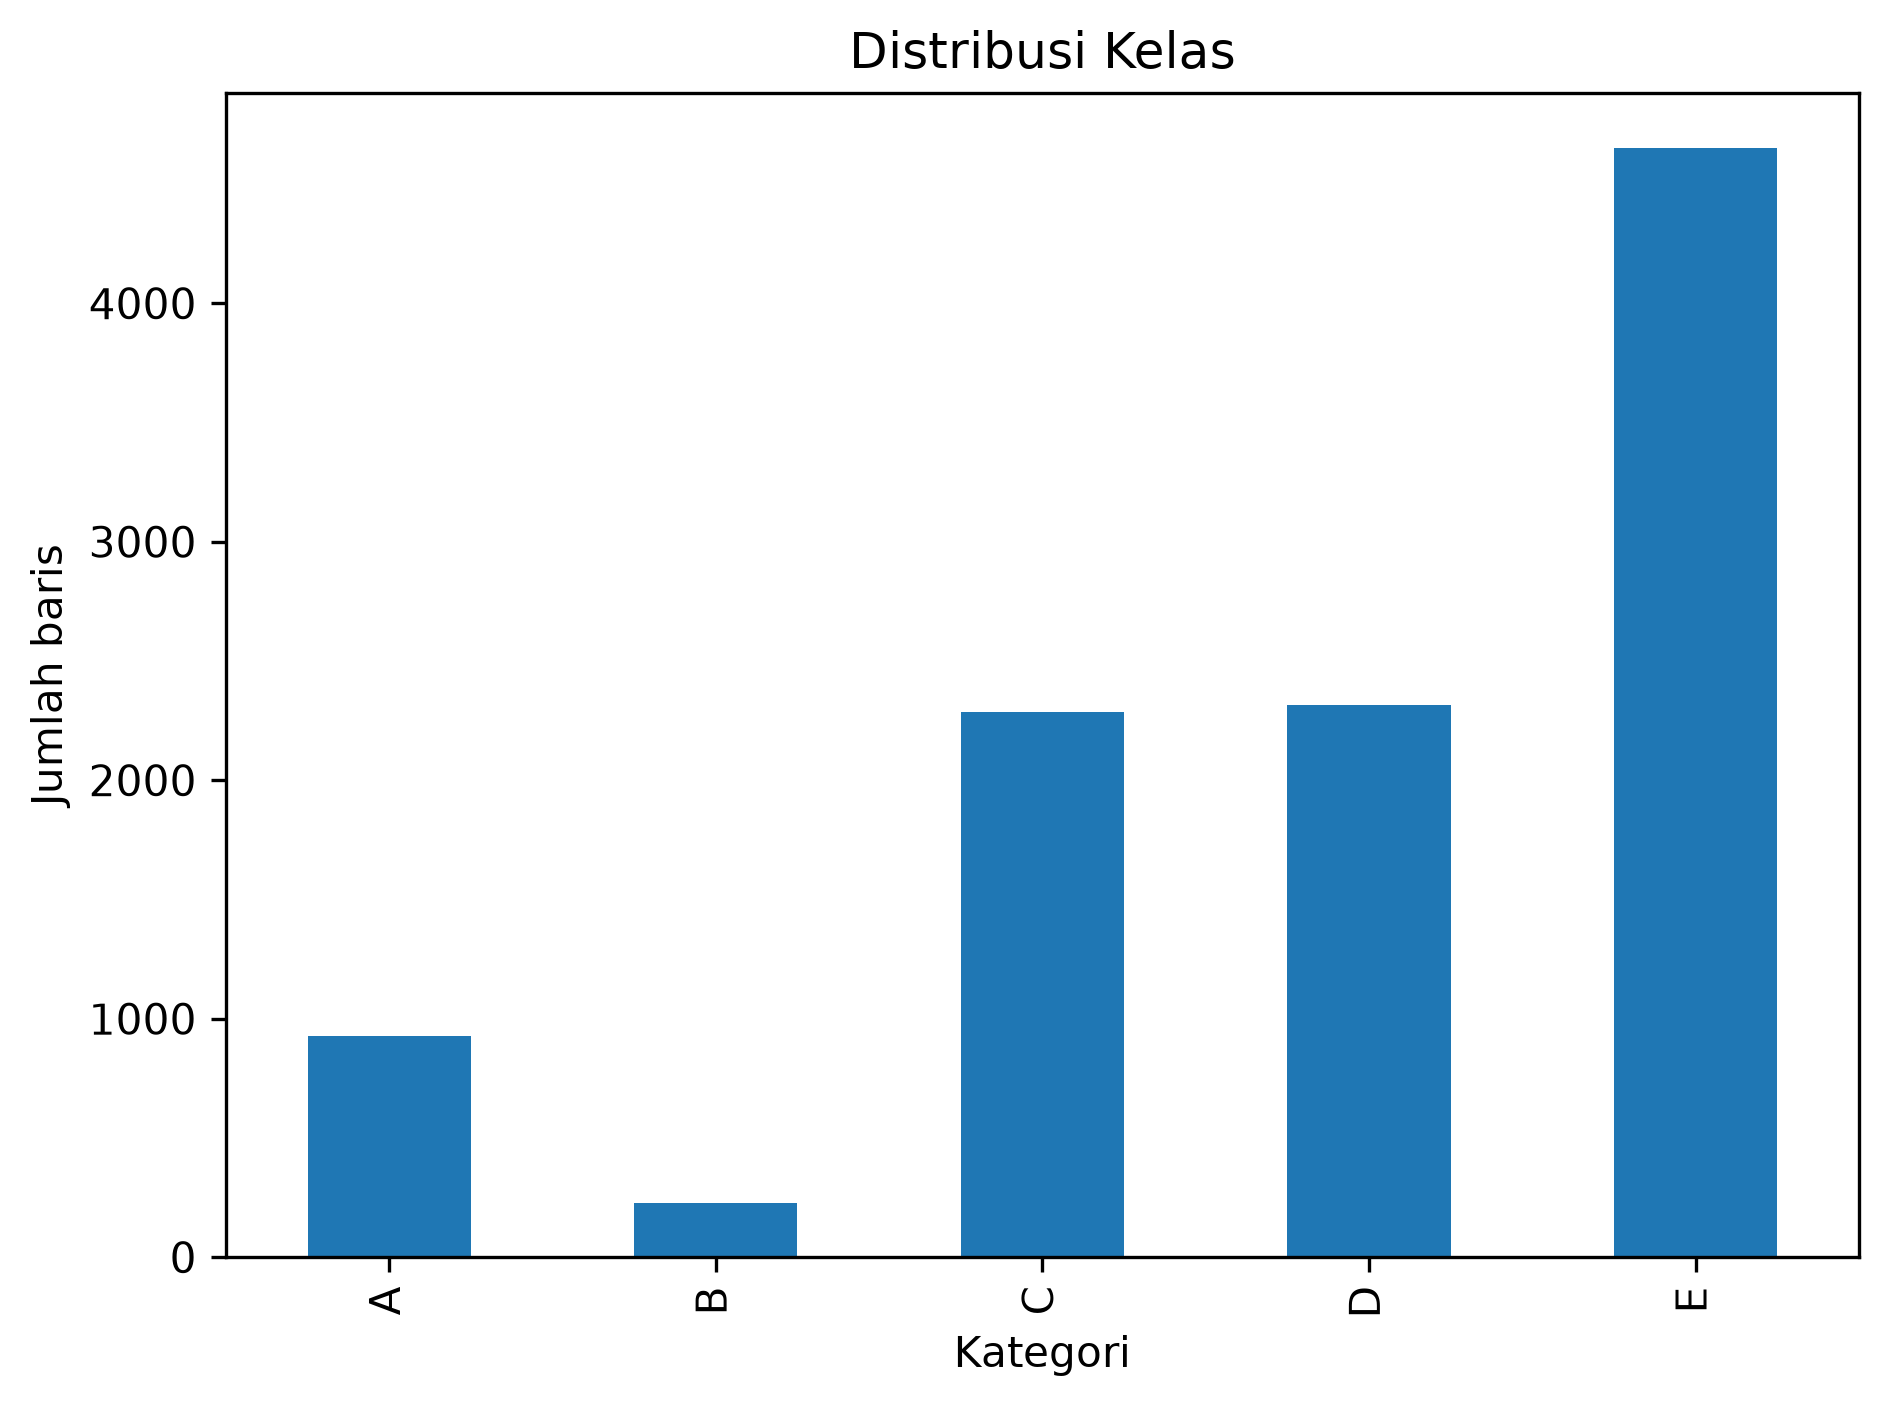
\includegraphics[width=\linewidth]{figure/out-new/01_distribusi_kelas.png}
\caption{Per-class row count of the raw e-nose dataset before preprocessing, showing the extreme class imbalance in which grade E dominates while the minority grade B is scarce (a ratio of $\approx$ 20:1).}
\label{fig:class_dist}
\end{figure}

\subsection{Data Leakage and Group-Aware Cross-Validation}
\label{subsec:cv}

The grouped structure can lead into potential data-leakage risk, since around forty rows that belonging to a single \textit{Sampling\_ID} are almost identical to one another. The average within-group feature standard deviation is only 5.5\%--22.5\% of the overall feature standard deviation. A traditional per-row random split would distribute these near-identical rows into both the training and test partitions. This method will lead to an overly optimistic performance estimation that is not valid since the test data already been observed before.

To prevent this leakage, all models are evaluated with \textit{StratifiedGroupKFold} grouped by \textit{Sampling\_ID}. This scheme will address every row with same \textit{Sampling\_ID} to a single fold, so the near-duplicate rows never splitted into train/test boundary and the model is always tested on physically unseen samples. It is also simultaneously \textit{stratified}, ensuring the proportions of data in the five classes match their original proportions in each fold, which is essential under the 20:1 imbalance because an unstratified split could otherwise leave a minority grade almost absent from a fold. It was verified that no group appears in more than one fold. The intersection of the training and test group sets is empty for every foldm and all 10{,}409 rows are retained, with only the fold boundaries made group-aware.

Fig.~\ref{fig:fold_proportion} confirms that the resulting class proportions in the training and test partitions remain nearly identical across all five folds, so each fold is representative of the full distribution despite the joint group-and-stratification constraint.

\begin{figure}[htbp]
\centering
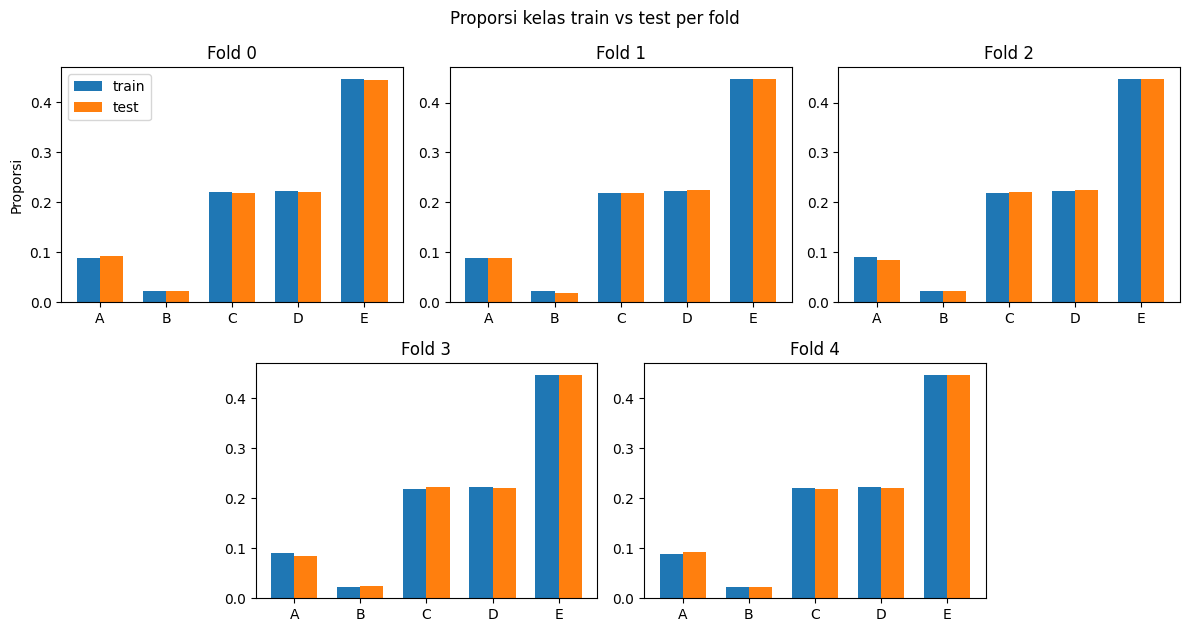
\includegraphics[width=\linewidth]{figure/out-new/02_proporsi_kelas_per_fold.png}
\caption{Class proportions of the training versus test partitions in each of the five folds. Stratification is preserved across folds even though the split is group-aware (by \textit{Sampling\_ID}).}
\label{fig:fold_proportion}
\end{figure}

\subsection{Preprocessing Pipeline}
\label{subsec:preprocessing}

The categorical target is first encoded to integers $0$--$4$ with \textit{LabelEncoder}. Within each training fold, the features are standardized with \textit{StandardScaler} (zero mean, unit variance) and then projected with Principal Component Analysis (PCA). Both the scaler and PCA are fitted only on the training partition of each fold and merely applied to the validation partition. This is enforced by wrapping the entire flow in a single scikit-learn \textit{Pipeline} (\textit{Scaler}~$\rightarrow$~\textit{PCA}~$\rightarrow$~\textit{Model}), which guarantees that no validation-fold statistics leak into the preprocessing during cross-validation or the learning-curve analysis.

Standardization is indispensable here because the twelve sensors operate on widely different physical scales. As Fig.~\ref{fig:normalization} shows, the raw feature ranges span from tens (humidity and temperature) to several hundreds (e.g., TGS813 and TGS2603); left unscaled, such large-magnitude sensors would dominate both the variance captured by PCA and the distance computations of the kernel and neural models. After \textit{StandardScaler}, every feature is reduced to a common zero-mean, unit-variance $z$-score, placing all sensors on an equal footing before dimensionality reduction.

\begin{figure}[htbp]
\centering
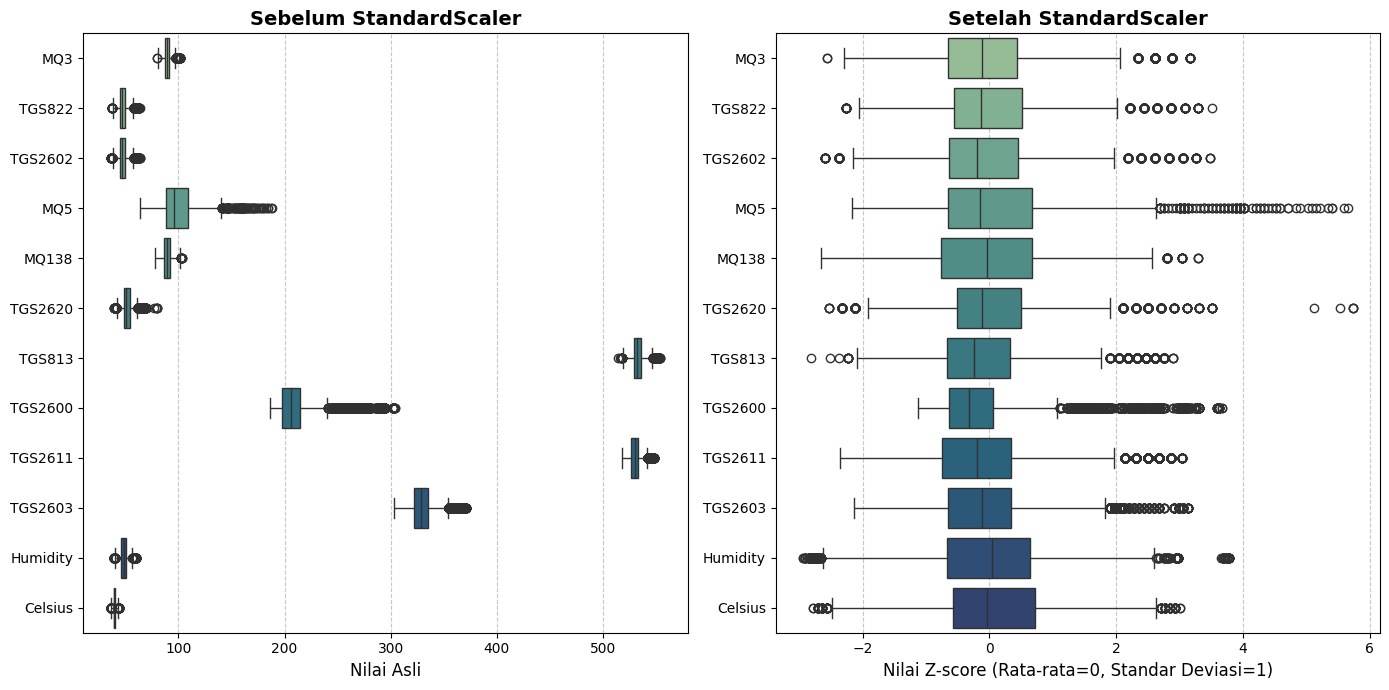
\includegraphics[width=\linewidth]{figure/normalization.png}
\caption{Per-feature value distributions before (left) and after (right) \textit{StandardScaler}. The disparate raw sensor scales are normalized to a common zero-mean, unit-variance $z$-score.}
\label{fig:normalization}
\end{figure}

The number of retained principal components is treated as a tuned hyperparameter, swept over $n_{\text{PCA}}\in\{3,5,8,12\}$. This choice is central to the study because, for the quantum models, the number of PCA components equals the number of qubits ($n_{\text{qubits}}=n_{\text{PCA}}$); sweeping the PCA dimension therefore jointly controls the classical input dimensionality and the quantum circuit width, keeping the paradigms comparable. The cumulative explained variance is 93.6\% at $n=5$, 98.3\% at $n=8$, and 100\% at $n=12$. Class imbalance is addressed without resampling: the SVM-based models use \textit{class\_weight}~$=$~`balanced', CatBoost uses \textit{auto\_class\_weights}~$=$~`Balanced', and the deep networks apply per-fold balanced class weights in the loss. No synthetic oversampling (e.g., SMOTE) is used, so all kernels and probability estimates are computed on the true data distribution.

PCA is employed as a linear dimensionality-reduction step that re-expresses the twelve correlated sensor features as mutually orthogonal components ordered by explained variance. It serves two purposes: it denoises and decorrelates the sensor signal, and---uniquely in this study---it sets the qubit count of the quantum circuits. Fig.~\ref{fig:pca_scatter} projects one fold onto its first two principal components and exposes the core difficulty of the task. The training and test partitions occupy the same region, confirming that the group-aware split is representative; however, the grades overlap substantially, with the adjacent grades A, D, and E heavily intermixed near the center while B and C form comparatively tighter clusters. This strong class overlap in the low-dimensional projection is precisely what motivates embedding the data into a higher-dimensional feature space, whether through nonlinear classical kernels or the quantum feature maps introduced later.

\begin{figure}[htbp]
\centering
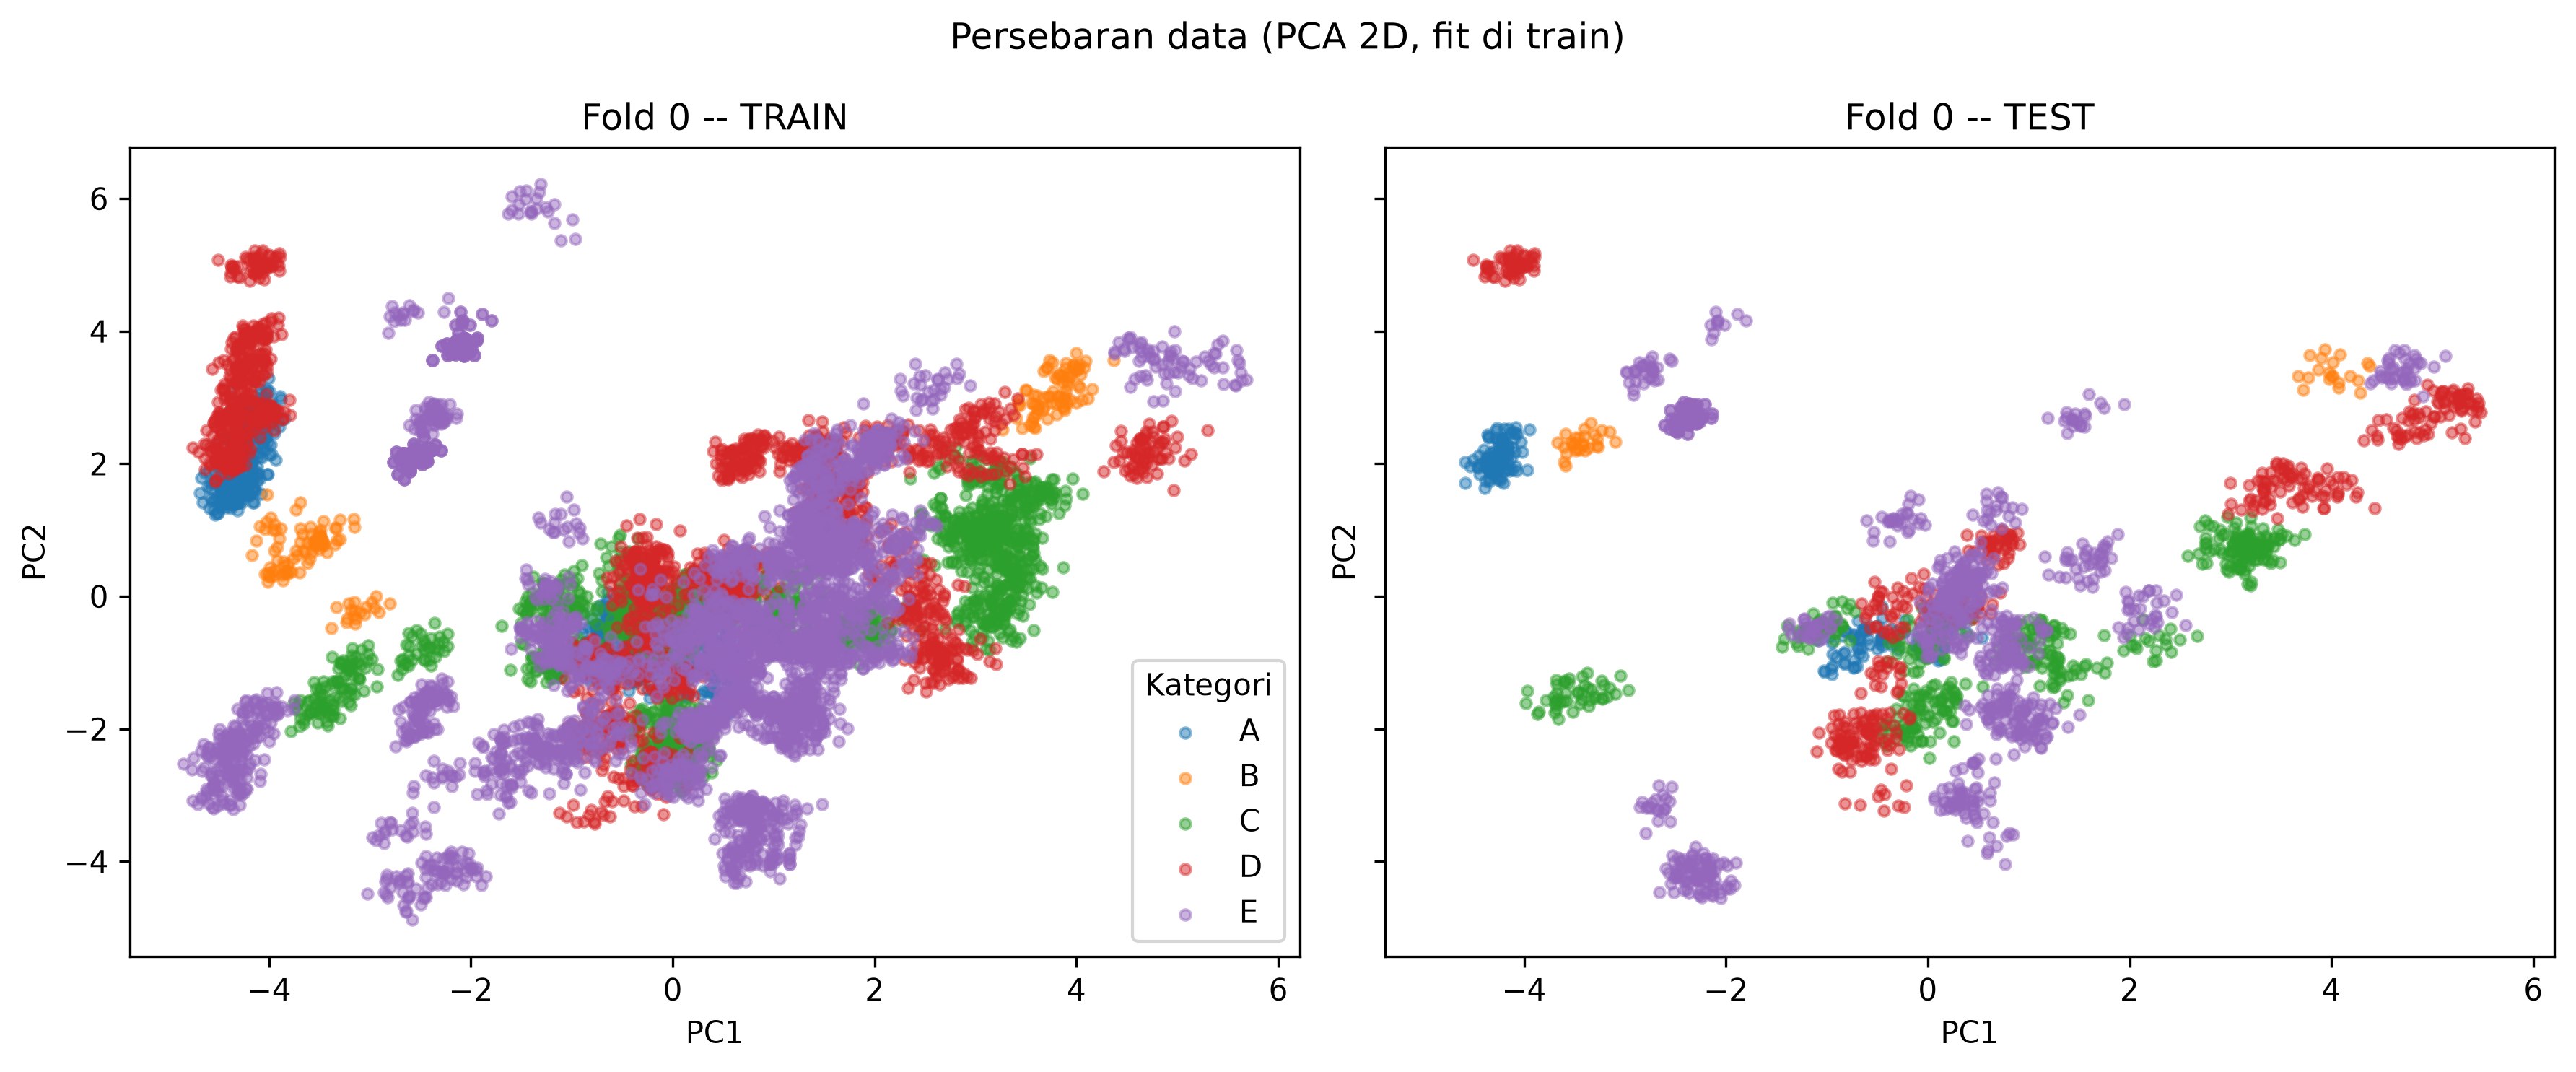
\includegraphics[width=\linewidth]{figure/out-new/03_pca2d_train_test.png}
\caption{Two-dimensional PCA projection (fitted on the training fold) of the training (left) and test (right) partitions. The partitions cover the same region, but grades A, D, and E overlap heavily, illustrating the non-linear separability of the e-nose data.}
\label{fig:pca_scatter}
\end{figure}

To set the range of the PCA sweep, the mean Composite score averaged over all models is examined as a function of the number of retained components (Fig.~\ref{fig:composite_pca}). Performance rises monotonically from 0.686 at $n=3$ to 0.847 at $n=12$, indicating that every additional principal component still carries discriminative information and that no intermediate value is clearly optimal. The full range up to $n_{\text{PCA}}=12$ (i.e., no reduction) is therefore retained in the sweep; the per-model resolution of this trend, which confirms that the leading models all select $n_{\text{PCA}}=12$, is analyzed in Section~\ref{sec:results}.

\begin{figure}[htbp]
\centering
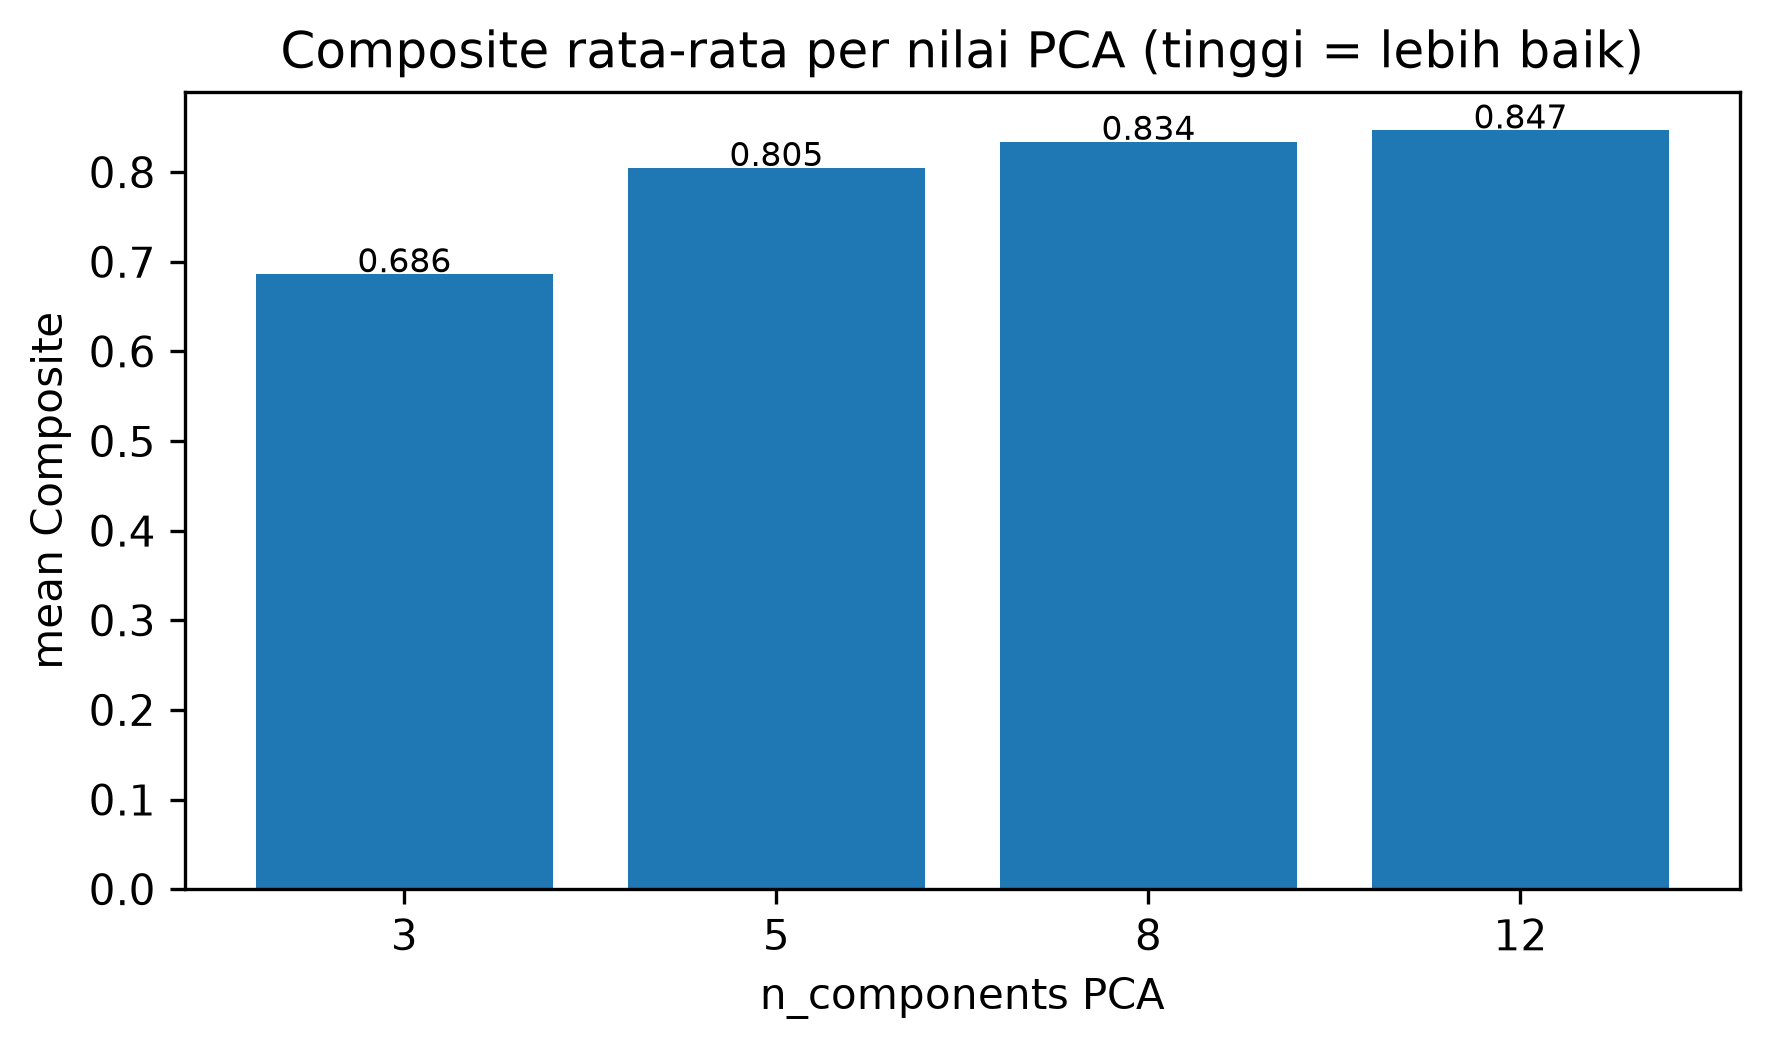
\includegraphics[width=\linewidth]{figure/out-new/04_composite_per_pca.png}
\caption{Mean Composite score (averaged over all models) as a function of the number of retained PCA components. Performance increases monotonically with dimensionality, peaking at $n_{\text{PCA}}=12$.}
\label{fig:composite_pca}
\end{figure}

\subsection{Evaluation Metrics and Composite Score}
\label{subsec:metrics}

For each fold, seven metrics are computed: Accuracy, macro-averaged Precision, macro-averaged Recall, macro-F1, the Matthews Correlation Coefficient (MCC), the one-vs-rest macro Area Under the Receiver Operating Characteristic curve (AUROC), and the one-vs-rest macro Area Under the Precision--Recall Curve (PRAUC). Every figure reported in this paper is the mean across the five folds.

Because the dataset is severely imbalanced, model selection is not driven by accuracy. Instead, a single minority-aware \textit{Composite} score is used as the selection criterion,
\begin{equation}
\mathrm{Composite} = \tfrac{1}{3}\Big(\text{macro-F1} + \tfrac{\mathrm{MCC}+1}{2} + \mathrm{PRAUC}\Big),
\label{eq:composite}
\end{equation}
which equally weights three complementary aspects: decision quality that counts every class equally (macro-F1), the balanced correlation of the full confusion matrix (MCC, rescaled from $[-1,1]$ to $[0,1]$), and probability-ranking quality that is sensitive to the minority classes (PRAUC). Accuracy and AUROC are reported for completeness but are deliberately excluded from the selection criterion because both are optimistically biased toward the majority class under severe imbalance. The Composite is a relative ranking score whose component zero-points differ, so it is always interpreted alongside its raw constituent metrics.

\subsection{Classical Baseline Models}
\label{subsec:classical_methods}

The classical baselines span two families. The first is the Support Vector Classifier (SVC) evaluated with four kernels---linear, radial basis function (RBF), polynomial, and sigmoid---which reveals how much of the problem is linearly separable and how much requires a nonlinear feature space. The second is gradient-boosted decision-tree ensembles, namely XGBoost (with both the \textit{gbtree} and \textit{dart} boosters) and CatBoost, which are among the strongest classical methods for tabular data. The tuned hyperparameter grids are listed in Table~\ref{tab:classical_grid}; every configuration additionally sweeps the PCA dimension.

\begin{table}[htbp]
\caption{Hyperparameter Grids of the Classical Baseline Models}
\label{tab:classical_grid}
\centering
\resizebox{\columnwidth}{!}{
    \begin{tabular}{l l}
    \hline
    \textbf{Model} & \textbf{Hyperparameter grid} \\
    \hline
    SVC-linear & $C\in\{0.01,0.1,1,10,100\}$ \\
    SVC-rbf & $C\in\{0.1,1,10,100\}$, $\gamma\in\{$scale$,0.01,0.1\}$ \\
    SVC-poly & $C\in\{1,10\}$, degree$\in\{2,3,4\}$, $\gamma\in\{$scale$,0.1\}$ \\
    SVC-sigmoid & $C\in\{0.1,1,10\}$, $\gamma\in\{$scale$,0.01,0.1\}$ \\
    XGBoost & $n_{\text{est}}\in\{200,400\}$, depth$\in\{3,6\}$, lr$\in\{0.05,0.1,0.3\}$, $\lambda_{\text{reg}}\in\{1,10\}$ \\
    CatBoost & depth$\in\{4,6\}$, lr$\in\{0.03,0.05,0.1\}$, iter$\in\{300,500\}$, $l2\in\{3,5,10\}$ \\
    \hline
    \multicolumn{2}{l}{\footnotesize All models additionally sweep $n_{\text{PCA}}\in\{3,5,8,12\}$.} \\
    \end{tabular}
}
\end{table}

\subsection{Deep Learning Baseline Models}
\label{subsec:dl_methods}

Two neural architectures serve as high-capacity, classical-hardware comparators. The Multilayer Perceptron (MLP) is a fully connected network with three hidden blocks (Dense $128\!\rightarrow\!64\!\rightarrow\!32$, ReLU activation, \textit{he\_normal} initialization), each followed by batch normalization and dropout of 0.2, terminating in a five-way softmax. The one-dimensional Convolutional Neural Network (1D-CNN) treats the PCA components as a single-channel sequence and stacks two convolutional blocks ($\text{Conv1D}(64,k{=}3)$ then $\text{Conv1D}(128,k{=}3)$, each with batch normalization, max-pooling, and dropout of 0.2), followed by global average pooling and a dense head. Both networks are trained with the Adam optimizer (learning rate $10^{-3}$), $L_2$ weight decay of $10^{-4}$, a batch size of 64, and up to 100 epochs with EarlyStopping (patience 15, restoring the best weights) on a stratified 15\% internal validation split. To keep the comparison strictly fair, the architectures are fixed at their best previously identified configurations and only the PCA dimension is swept, exactly as for the other paradigms.

\subsection{Quantum Kernel Models}
\label{subsec:quantum_methods}

\subsubsection{Quantum Feature Maps and Kernel Estimation}
A quantum kernel classifier embeds each classical input $x$ into an $n$-qubit quantum state $|\phi(x)\rangle = U_{\text{enc}}(x)\,|0\rangle^{\otimes n}$ through a parameterized feature-map circuit $U_{\text{enc}}$, and then trains a classical Support Vector Machine on a kernel matrix computed from these states; this is the QSVC model. The conventional fidelity-based estimator (Quantum Kernel Estimation) defines the kernel as the state overlap $|\langle\phi(x_i)|\phi(x_j)\rangle|^2$, which requires $O(N^2)$ circuit evaluations for $N$ samples and is therefore intractable on the full 10{,}409-row dataset.

\subsubsection{Projected Quantum Kernel}
To make a full-dataset, leakage-free comparison feasible, all quantum models in this study use the Projected Quantum Kernel (PQK) introduced by Huang \textit{et al.}\ rather than a fidelity kernel. The PQK projects each encoded state onto its single-qubit reduced density matrices, retaining the three Pauli expectation values per qubit, $\rho_k(x)=[\langle X_k\rangle, \langle Y_k\rangle, \langle Z_k\rangle]$, to form a $3n$-dimensional projected feature vector, and then applies a classical RBF kernel in that projected space,
\begin{equation}
k_{\text{PQ}}(x_i,x_j) = \exp\!\Big(-\gamma \sum_{k=1}^{n} \big\lVert \rho_k(x_i)-\rho_k(x_j) \big\rVert_F^2\Big).
\label{eq:pqk}
\end{equation}
This reduces the quantum cost to $O(N)$ statevector evaluations, which is precisely what allows the quantum models to be run on all 10{,}409 rows without subsampling and thus compared fairly against the classical and deep learning baselines. The PQK bandwidth $\gamma$ controls the width of the projected-space RBF: a smaller $\gamma$ widens the kernel and counteracts \textit{kernel concentration}, the regime in which all pairwise kernel values become nearly uniform and the kernel ceases to discriminate.

\subsubsection{Feature Map Designs}
\label{subsubsec:featuremaps}
Three scale controls are shared across feature maps: an entanglement scale $\lambda=0.1$, an input bandwidth $c$ that rescales every rotation angle to $c\,x_i$ (a second mechanism against kernel concentration), and the number of re-uploading layers \textit{reps} for the re-uploading family. The entangling topologies are \textit{full} (all qubit pairs), \textit{linear} (a nearest-neighbor chain), and \textit{circular} (a ring). The following feature maps are evaluated:

\begin{itemize}
\item \textbf{Baseline IQP.} The standard Instantaneous Quantum Polynomial map applies $H$ then $R_Z(x_i)$ on each qubit, followed by $R_{ZZ}(\lambda\,x_i x_j)$ on the entangling pairs. Because this activates only the $\langle Z\rangle$ projection, two of the three Pauli features per qubit are wasted under the PQK. Pure single-axis encodings ($R_X$-, $R_Y$-, $R_Z$-only) and several phase-encoding variants (cosine, quadratic, polynomial) were also screened as diagnostic controls.
\item \textbf{star.} A lightweight map with single-hub (star) entanglement: after an $H,R_Z(x_i)$ encoding, a hub qubit is entangled with each remaining qubit $j$ through a $\text{CX}$--$\{R_X,R_Y,R_Z\}$--$\text{CX}$ block, making it already multi-basis while keeping only $n-1$ entangling blocks.
\item \textbf{REUP-HE (v1--v3).} A re-uploading hardware-efficient family that adds multi-basis rotations ($R_Y$ then $R_Z$), data-dependent entanglement, bandwidth $c$, and \textit{reps}~$=2$ re-uploading layers. Variant v1 uses data-dependent $R_{ZZ}$ entanglement; v2 uses dense multi-basis entanglement on all topology pairs; and v3 (\textit{lite}) keeps a single rotating hub per layer.
\item \textbf{Proposed STAR-v2.} The proposed feature map upgrades \textit{star} with three targeted modifications while deliberately preserving its light single-hub entanglement: (i) a richer multi-basis state preparation $H,\,R_Y(c\,x_i),\,R_Z(c\,x_i)$ that makes all three Pauli expectations $\langle X\rangle,\langle Y\rangle,\langle Z\rangle$ informative from the outset; (ii) the bandwidth $c=0.5$ applied to every rotation angle; and (iii) the single-hub entanglement retained unchanged. For hub $h{=}0$ and each $j\neq 0$, the entangling block is $\text{CX}_{0,j}$, $R_X(c\lambda x_0)$, $R_Y(c\lambda x_0 x_j)$, $R_Z(c\lambda x_j)$, $\text{CX}_{0,j}$, which moves the $x_0 x_j$ interaction term onto the $Y$ basis.
\end{itemize}

\subsubsection{Quantum-Boosted Hybrid Models}
Two hybrid models test whether the quantum kernel is more effective used directly or as engineered features. QCAT and QXGB feed the projected quantum kernel---compressed through a Nystr\"om approximation---as input features into CatBoost and XGBoost, respectively, rather than into an SVM.

\subsection{Hyperparameter Optimization and Search Spaces}
\label{subsec:hpo}

Hyperparameters are tuned by exhaustive Grid Search: every combination in the predefined grid is scored by the full 5-fold group-aware cross-validation, and the configuration with the highest mean Composite is selected. The same procedure is applied to all paradigms so that the comparison reflects each model at its best. For the classical models the grids of Table~\ref{tab:classical_grid} apply; for the deep networks only the PCA dimension is swept. For the quantum models the tuned hyperparameters are the SVM regularization $C$, the PCA dimension (equivalently the qubit count), and---in the final experiments---the PQK bandwidth $\gamma\in\{0.25,0.5\}$, while the circuit constants ($\lambda=0.1$, $c=0.5$, \textit{reps}~$=2$) are held fixed so that the quantum search space remains comparable in size to the classical one. Table~\ref{tab:quantum_grid} summarizes the quantum search space. All runs are checkpointed so that an interrupted search resumes without re-evaluating completed configurations.

\begin{table}[htbp]
\caption{Quantum Model Search Space (PQK, $\lambda=0.1$, $c=0.5$)}
\label{tab:quantum_grid}
\centering
\resizebox{\columnwidth}{!}{
    \begin{tabular}{l l l}
    \hline
    \textbf{Family} & \textbf{Feature maps} & \textbf{Tuned grid} \\
    \hline
    IQP baseline & full, linear, circular & $C\in\{1\}$ \\
    Encoding controls & $x/y/z$, cosine, quadratic, poly. & $C\in\{1,10\}$ \\
    star & star & $C\in\{1,10\}$, $\gamma\in\{0.25,0.5,1\}$ \\
    REUP-HE v1 & reup\_\{full,linear,circular\} & $C\in\{1\}$ \\
    REUP-HE v2 & reup\_ent\_\{full,linear,circular\} & $C\in\{1,10\}$ \\
    REUP-HE v3 & reup\_lite & $C\in\{1\}$, $\gamma\in\{0.25,0.5,1\}$ \\
    \textbf{STAR-v2} & \textbf{star\_v2} & $C\in\{1,10\}$, $\gamma\in\{0.25,0.5\}$ \\
    Hybrid & QCAT, QXGB & tree depth \\
    \hline
    \multicolumn{3}{l}{\footnotesize All sweep $n_{\text{PCA}}=n_{\text{qubits}}\in\{3,5,8,12\}$.} \\
    \end{tabular}
}
\end{table}

\section{Results and Discussion}
\label{sec:results}

This section reports the empirical evaluation of the three modeling paradigms considered in this study---classical machine learning, deep learning, and quantum kernel methods---under a single, identical protocol so that every comparison is strictly apple-to-apple. All models are evaluated on the full e-nose dataset (10{,}409 spectra, 12 gas-sensor features, and five quality grades A, B, C, D, and E, using a group-aware \textit{StratifiedGroupKFold} (5 folds, grouped by \textit{Sampling\_ID}) that eliminates the inter-row leakage induced by the clustered acquisition structure, in which the 10{,}409 rows originate from only 69 physical tea samples. Preprocessing (\textit{StandardScaler} followed by Principal Component Analysis) is fitted exclusively on each training fold inside a pipeline, and the number of PCA components---which simultaneously defines the number of qubits for the quantum models---is swept over $\{3,5,8,12\}$. Because the dataset is severely imbalanced (a class ratio of E:B $\approx$ 20:1), model selection is driven by the minority-aware Composite score defined in~\eqref{eq:composite}, which equally weights decision quality (macro-F1), the balanced correlation of the full confusion matrix (MCC, rescaled to $[0,1]$), and probability-ranking quality on minority classes (PRAUC). Accuracy and the Area Under the Receiver Operating Characteristic curve (AUROC) are reported for completeness but are deliberately excluded from the selection criterion because they are optimistically biased toward the majority class under imbalance. All reported figures are mean values across the five folds. The full evaluation protocol is detailed in Section~\ref{sec:methodology}.

\subsection{Performance of Classical Models}

This section reports the performance of all classical-hardware baselines, which together form the comparison foundation against the quantum kernels introduced in the next section. Two complementary model families are considered. The first comprises the conventional classical machine learning baselines (kernel SVMs and gradient-boosted trees), and the second comprises deep learning baselines, namely a Multilayer Perceptron (MLP) and a one-dimensional Convolutional Neural Network (1D-CNN). Deep learning is deliberately included as an additional, strong non-quantum reference: because deep neural networks are the dominant high-capacity approach to nonlinear modeling and are frequently among the most competitive methods on complex problems, a fair quantum-versus-classical claim must hold not only against classical machine learning but also against a properly tuned deep network. To keep the comparison strictly apple-to-apple, both deep learning models are evaluated under the identical protocol used for every other model---the same group-aware 5-fold cross-validation, the same PCA sweep over $\{3,5,8,12\}$, the same per-fold class weighting in place of resampling, and the same minority-aware Composite selection criterion.

Table \ref{tab:classical_models} presents the empirical performance of both families. Among the classical machine learning baselines, tree-based ensembles (XGBoost, CatBoost) and the Support Vector Classifier with a non-linear kernel (SVC-rbf) yield the strongest performance. Specifically, the CatBoost model achieves the highest classical machine learning Composite score of 0.9379, closely followed by SVC-rbf at 0.9378---a difference of only 0.0001, far below the inter-fold standard deviation, so the two are best regarded as a statistical tie. The strongest deep learning model, the MLP, reaches a Composite of 0.9392, marginally ahead of the best classical machine learning model and therefore the highest score among all classical-hardware baselines, while the 1D-CNN trails at 0.9307. The deep learning architectures are specified in Section~\ref{subsec:dl_methods} and their results discussed in Section~\ref{subsubsec:dl_baselines}.

The evaluation metrics demonstrate that both CatBoost and SVC-rbf are highly capable of navigating the extreme class imbalance inherent in the dataset. This robustness is particularly evident in their high minority-sensitive metrics, including a macro-F1 of approximately 0.91 and a Precision-Recall Area Under Curve (PRAUC) of nearly 0.97 for both models.

\begin{table}[htbp]
\caption{Performance Comparison of Classical and Deep Learning Models}
\label{tab:classical_models}
\centering
\resizebox{\columnwidth}{!}{
    \begin{tabular}{l c c c c c c}
    \hline
    \textbf{Model} & \textbf{Acc} & \textbf{Recall} & \textbf{F1} & \textbf{MCC} & \textbf{PRAUC} & \textbf{Composite} \\
    \hline
    \multicolumn{7}{l}{\textit{Classical Machine Learning}} \\
    \textbf{CatBoost} & 0.9076 & \textbf{0.9172} & \textbf{0.9124} & 0.8689 & 0.9669 & 0.9379 \\
    SVC-rbf & 0.9155 & 0.9132 & 0.9068 & 0.8800 & 0.9667 & 0.9378 \\
    XGBoost & 0.8979 & 0.8848 & 0.8934 & 0.8544 & 0.9519 & 0.9242 \\
    SVC-poly & 0.8278 & 0.8664 & 0.8229 & 0.7658 & 0.8920 & 0.8659 \\
    SVC-linear & 0.5378 & 0.6186 & 0.5029 & 0.4020 & 0.6203 & 0.6081 \\
    SVC-sigmoid & 0.4755 & 0.5720 & 0.4241 & 0.3467 & 0.4946 & 0.5307 \\
    \hline
    \multicolumn{7}{l}{\textit{Deep Learning}} \\
    \textbf{MLP} & \textbf{0.9178} & 0.8980 & 0.9025 & \textbf{0.8828} & \textbf{0.9737} & \textbf{0.9392} \\
    1D-CNN & 0.9058 & 0.8971 & 0.8934 & 0.8672 & 0.9651 & 0.9307 \\
    \hline
    \end{tabular}
}
\end{table}

The classical results also reveal the intrinsic distribution profile of the e-nose sensor data: the features that separate the tea quality grades are strongly non-linear. As shown in Table \ref{tab:classical_models}, SVC-linear and SVC-sigmoid suffer from severe underfitting, collapsing to Composite scores of only 0.6081 and 0.5307, respectively, whereas radial-basis and tree-based models thrive. This places the classical models into three clear tiers: a strong tier (CatBoost, SVC-rbf, XGBoost), an intermediate tier (SVC-poly), and a failing tier (SVC-linear, SVC-sigmoid). Fig.~\ref{fig:classical_boxplot} illustrates the per-fold stability of the leading models, with CatBoost and SVC-rbf maintaining tight distributions across folds.

\begin{figure}[htbp]
\centering
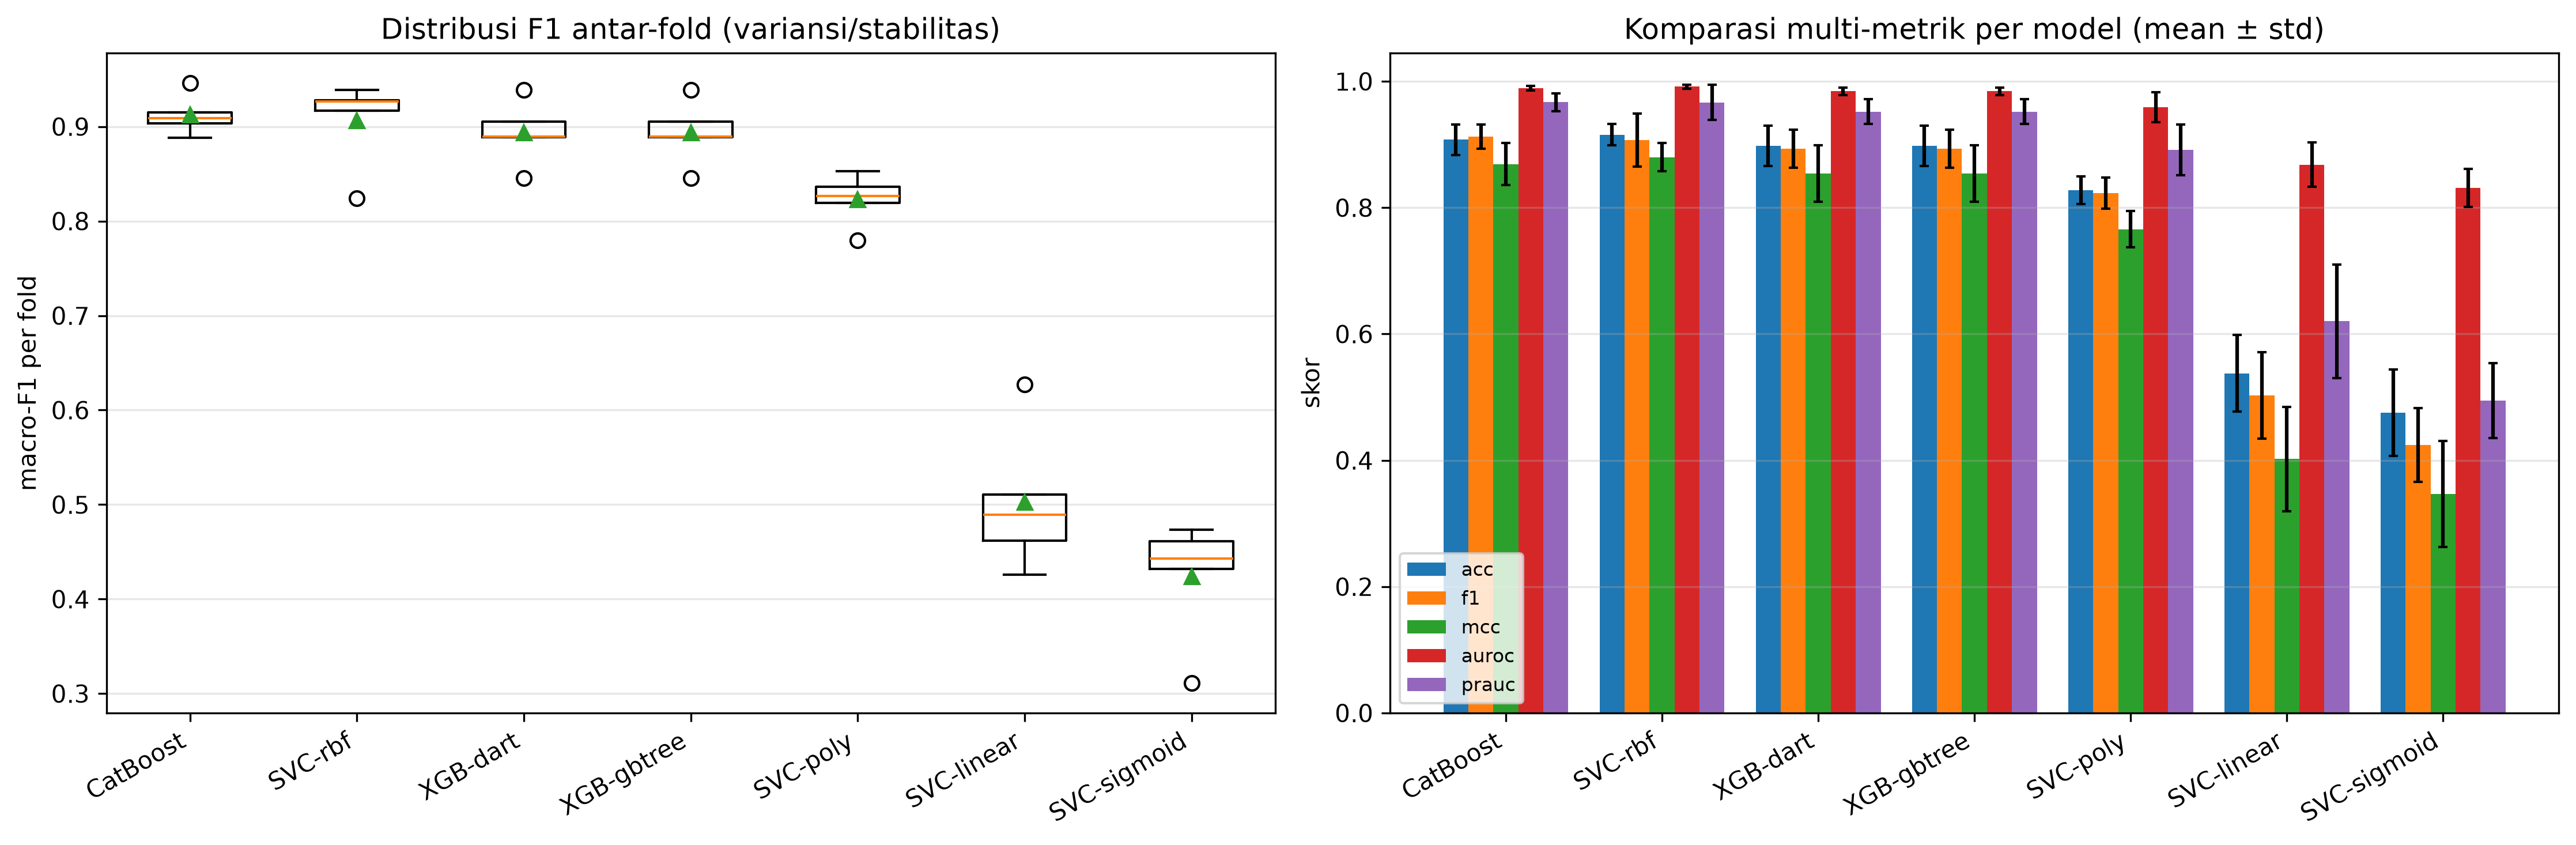
\includegraphics[width=\linewidth]{figure/out-new/14_box_perfold_multimetrik.png}
\caption{Performance distribution across validation folds, illustrating the stability of CatBoost and SVC-rbf compared to other classical approaches.}
\label{fig:classical_boxplot}
\end{figure}

A complementary view of the entire search is provided in Fig.~\ref{fig:classical_spread}, which plots the best Composite score per model together with the full distribution of all evaluated configurations. The strong tier not only reaches the highest peaks but also maintains a high median, indicating that their performance is not the product of a single lucky configuration. Fig.~\ref{fig:classical_pca_heatmap} further resolves the Composite score by model and PCA dimension; the warmest cells consistently appear at the highest dimensionality, confirming that all leading classical models select \mbox{$n_{\text{PCA}}=12$} (i.e., no dimensionality reduction), because additional principal components carry discriminative information that the models exploit.

\begin{figure}[htbp]
\centering
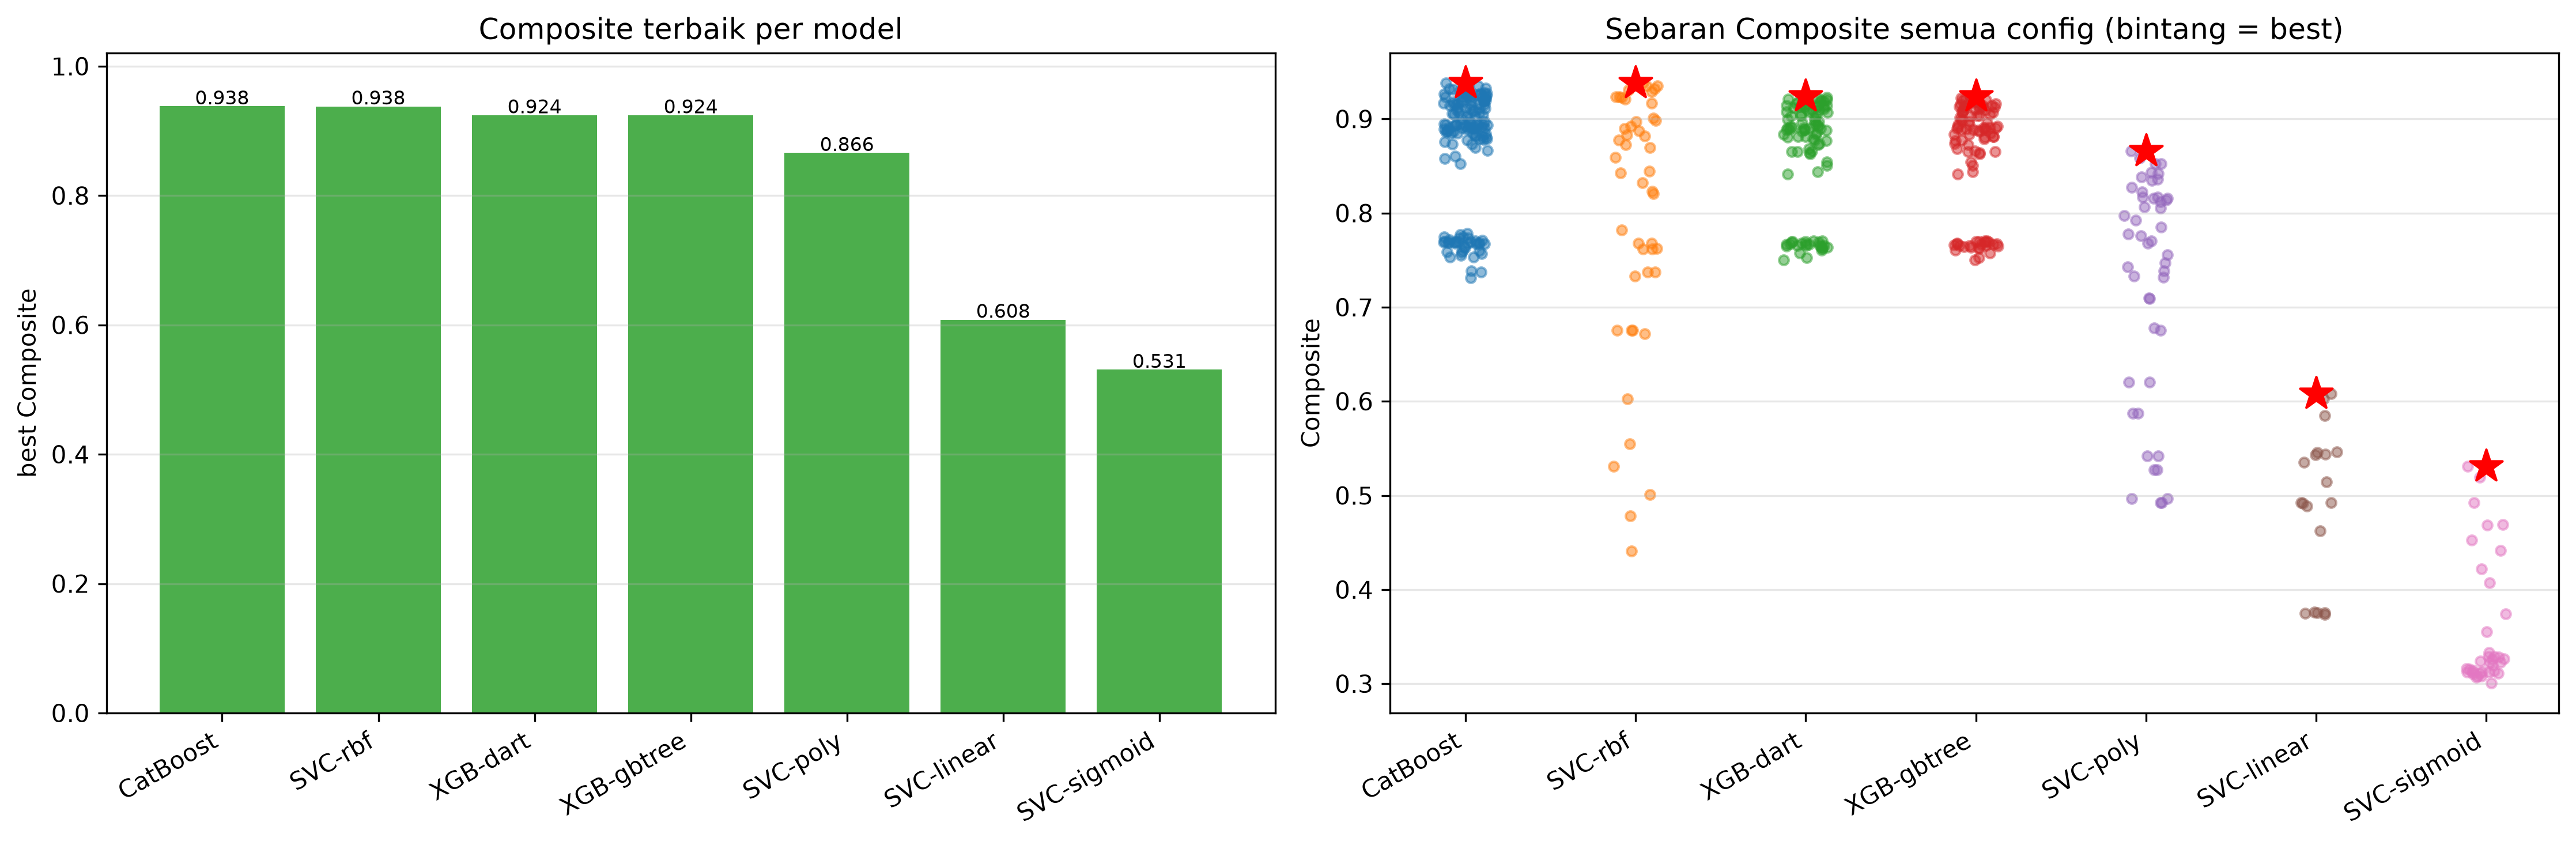
\includegraphics[width=\linewidth]{figure/out-new/15_composite_score_sebaran.png}
\caption{Best Composite score per classical model and the spread of all evaluated configurations, showing the clear separation between the strong, intermediate, and failing tiers.}
\label{fig:classical_spread}
\end{figure}

\begin{figure}[htbp]
\centering
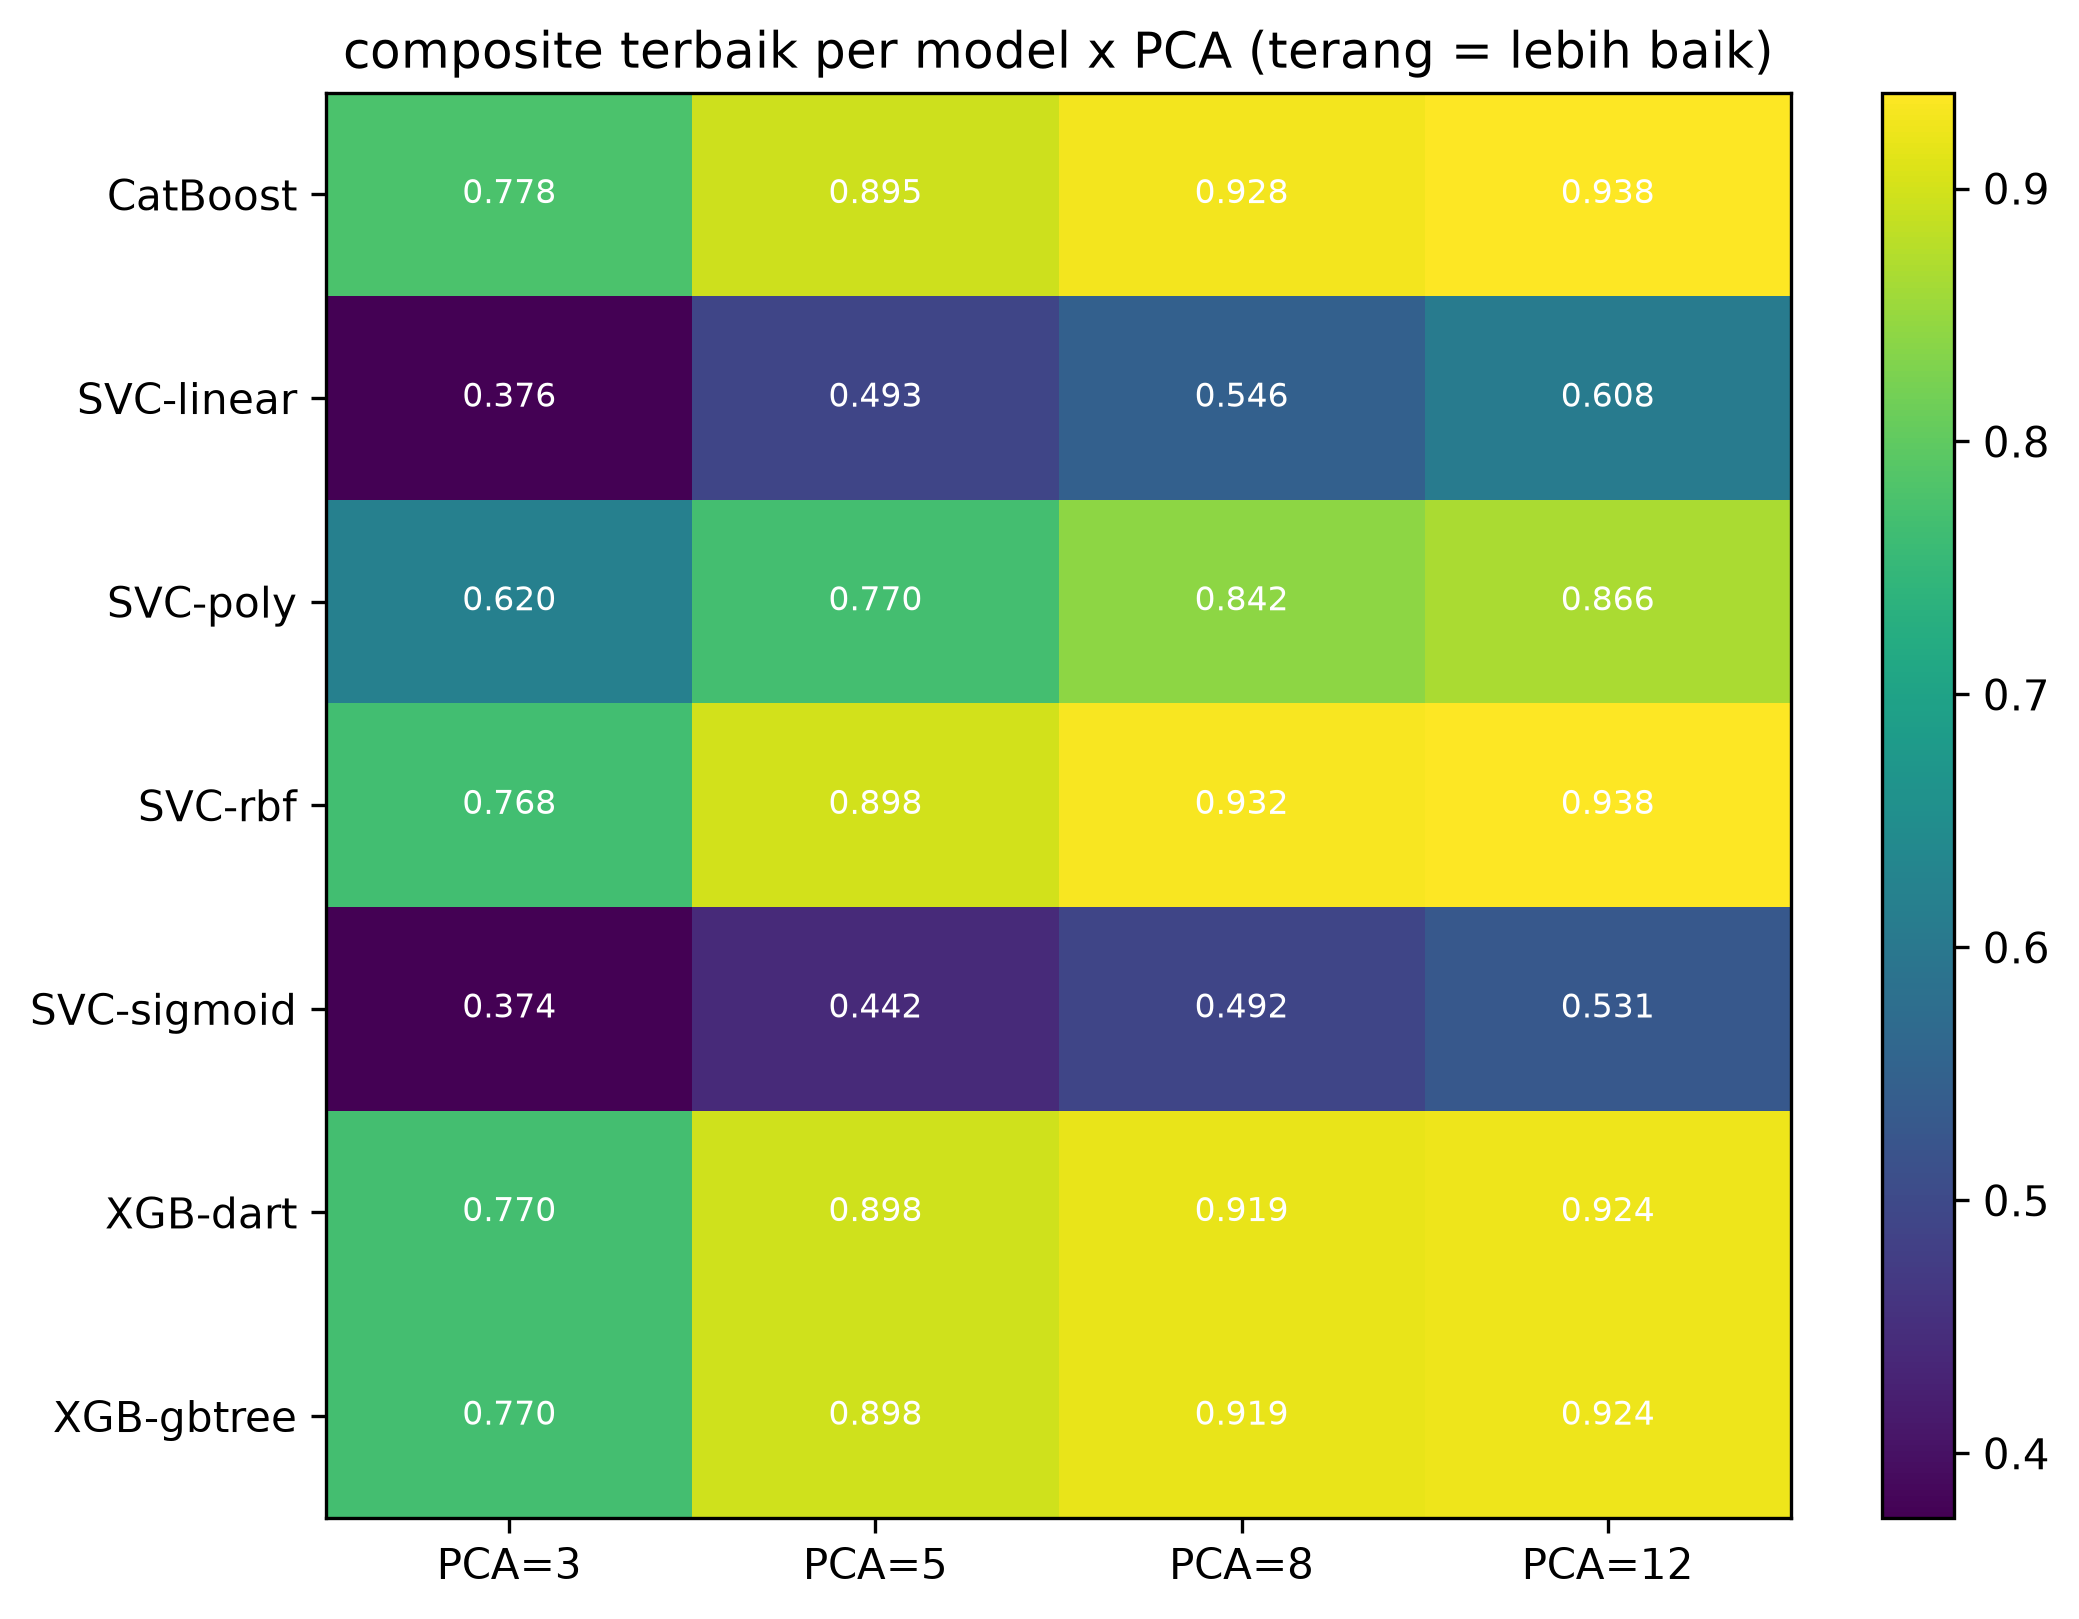
\includegraphics[width=\linewidth]{figure/out-new/05_heatmap_model_x_pca.png}
\caption{Composite score per classical model across PCA dimensions; performance increases monotonically with the number of retained components, with the optimum at $n_{\text{PCA}}=12$.}
\label{fig:classical_pca_heatmap}
\end{figure}

Beyond peak accuracy, the tuning efficiency of each model is summarized in Table \ref{tab:efficiency} and visualized in Fig.~\ref{fig:classical_efficiency}. SVC-rbf is the most tuning-efficient model, reaching a near-best Composite with the fewest configurations, whereas CatBoost is the most robust, achieving the highest mean Composite across the search space (so that even an arbitrary configuration performs well) at the cost of requiring more trials to lock in its very best result.

\begin{table}[htbp]
\caption{Search Efficiency of the Strong-Tier Classical Models}
\label{tab:efficiency}
\centering
\resizebox{\columnwidth}{!}{
    \begin{tabular}{l c c c c}
    \hline
    \textbf{Model} & \textbf{Best} & \textbf{Mean} & \textbf{\% Near-Best} & \textbf{Exp. \#Config} \\
    \hline
    CatBoost & 0.938 & \textbf{0.869} & 6.2\% & 16.0 \\
    \textbf{SVC-rbf} & 0.938 & 0.803 & \textbf{14.6\%} & \textbf{6.9} \\
    XGBoost & 0.924 & 0.862 & 12.5\% & 8.0 \\
    SVC-poly & 0.866 & 0.729 & 4.2\% & 24.0 \\
    \hline
    \end{tabular}
}
\end{table}

\begin{figure}[htbp]
\centering
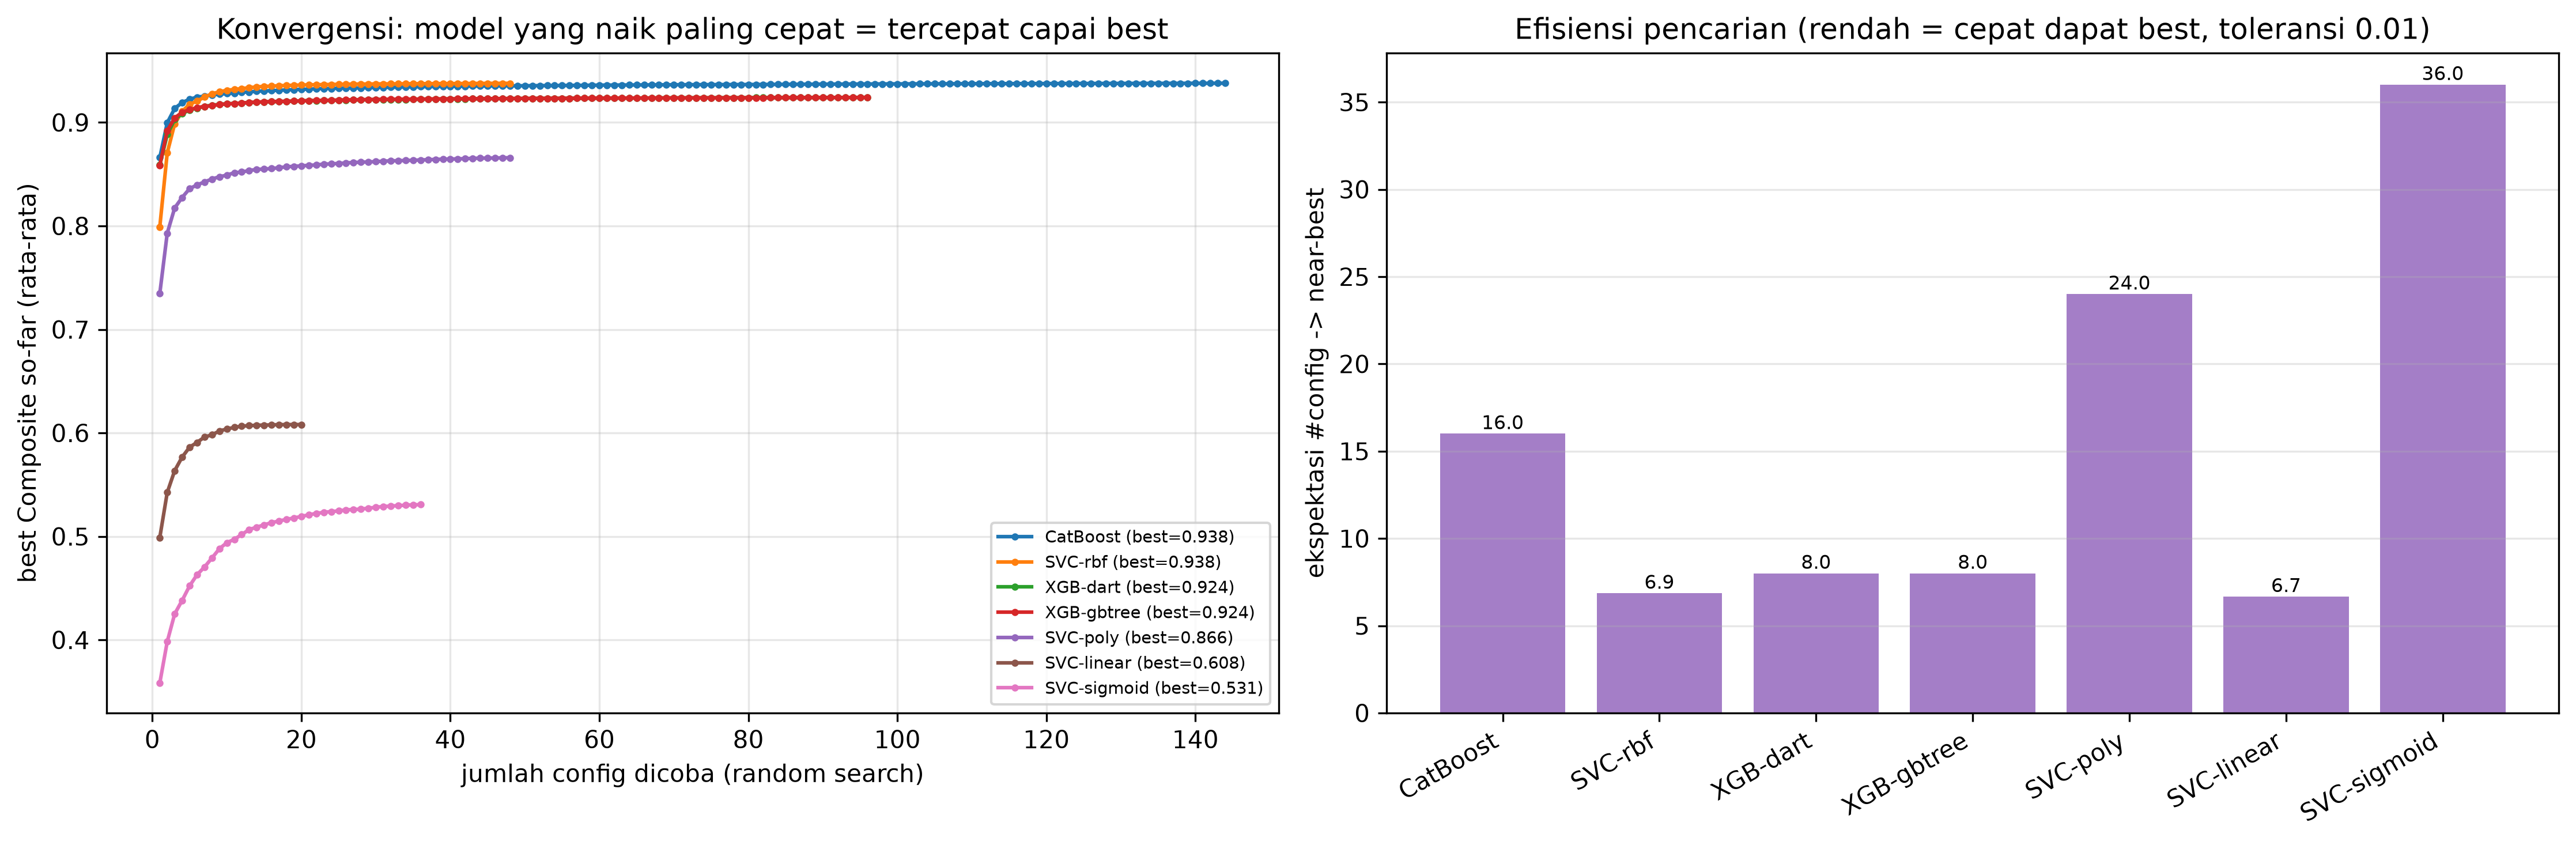
\includegraphics[width=\linewidth]{figure/out-new/16_konvergensi_efisiensi.png}
\caption{Random-search convergence and tuning efficiency per classical model, contrasting the fast convergence of SVC-rbf with the high average quality of CatBoost.}
\label{fig:classical_efficiency}
\end{figure}

\subsubsection{Deep Learning Baselines}
\label{subsubsec:dl_baselines}

Beyond the classical machine learning models, two deep learning architectures---the MLP and the 1D-CNN defined in Section~\ref{subsec:dl_methods}---are evaluated as additional high-capacity comparators, trained under the same group-aware protocol with the PCA dimension swept exactly as for the other paradigms and class imbalance handled by per-fold balanced class weights rather than resampling.

As reported in Table \ref{tab:classical_models}, the MLP is the stronger of the two deep networks, exceeding the 1D-CNN by $+0.0085$ in Composite. This ordering is expected: the PCA-projected sensor features form a genuinely tabular representation with no spatial or temporal locality for a convolutional kernel to exploit, so the inductive bias of the 1D-CNN confers no advantage and the dense MLP is the more appropriate model. The MLP also exhibits a distinctly precision-oriented profile (precision 0.9228 against recall 0.8980), attaining the highest precision and AUROC (0.9924) of any classical-hardware baseline---a profile that contrasts with the more recall-balanced CatBoost and, notably, resembles that of the quantum kernels analyzed later. Fig.~\ref{fig:dl_boxplot} confirms that this advantage is stable rather than fold-specific, with the MLP holding tight inter-fold distributions across all metrics, while Fig.~\ref{fig:dl_spread} shows that its leading Composite is sustained as a high median across the configuration sweep rather than arising from a single fortunate run.

\begin{figure}[htbp]
\centering

\includegraphics[width=\linewidth]{figure/qml/DL/14_box_perfold_multimetrik.png}
\caption{Per-fold multi-metric distribution of the deep learning models, illustrating the stability of the MLP relative to the 1D-CNN across the five validation folds.}
\label{fig:dl_boxplot}
\end{figure}

\begin{figure}[htbp]
\centering

\includegraphics[width=\linewidth]{figure/qml/DL/15_composite_score_sebaran.png}
\caption{Best Composite score per deep learning model and the spread of all evaluated configurations, confirming that the MLP leads the 1D-CNN by a consistent margin rather than at a single configuration.}
\label{fig:dl_spread}
\end{figure}

Like the classical models, both deep networks select \mbox{$n_{\text{PCA}}=12$} as optimal, with the MLP Composite rising monotonically across the PCA sweep ($0.776 \rightarrow 0.910 \rightarrow 0.934 \rightarrow 0.939$ for $n_{\text{PCA}}\in\{3,5,8,12\}$). This reaffirms, on an entirely different model family, that the discriminative information is distributed across all twelve principal components and that aggressive dimensionality reduction is harmful. The deep learning models therefore corroborate the same dataset-level conclusions drawn from the classical baselines, and together the two families constitute a strong, two-pronged classical-hardware benchmark against which the quantum kernels are assessed in the following section.

Consequently, CatBoost and SVC-rbf are established as the definitive classical benchmarks for this study, with the MLP as the strongest deep learning reference. Their strong non-linear feature-space projections provide a rigorous comparative foundation against which to evaluate the high-dimensional mapping capabilities of the proposed quantum circuits discussed in the subsequent sections.

\subsection{Performance of Quantum Models}

All quantum models in this study employ the Projected Quantum Kernel (PQK) rather than a fidelity kernel. Each sample is encoded into a quantum state through a feature map, the state is projected onto the single-qubit Pauli expectations $[\langle X_k\rangle, \langle Y_k\rangle, \langle Z_k\rangle]$ for every qubit $k$, yielding a $3n$-dimensional projected feature vector, and the final kernel is a radial basis function (RBF) evaluated in that projected space, $k(x_i,x_j)=\exp(-\gamma\sum_k \lVert \rho_k(x_i)-\rho_k(x_j)\rVert^2)$. A key practical consequence is that the PQK scales linearly with the number of samples, which is precisely what makes it feasible to run the quantum models on all 10{,}409 rows without subsampling and therefore to compare them fairly against the classical baselines.

Table \ref{tab:baseline_quantum} details the empirical results of the baseline quantum configurations, encompassing standard Instantaneous Quantum Polynomial (IQP) feature maps, an earlier multi-basis heuristic map (\textit{star}), and quantum-boosted hybrid trees (QCAT, QXGB). The results demonstrate that the direct kernel implementation (\textit{QSVC}) utilizing the \textit{star} feature map achieved the highest baseline quantum performance, securing a Composite score of 0.9287. This configuration significantly outperformed all topological variations of the standard IQP feature maps (\textit{Full}, \textit{Circular}, and \textit{Linear}), which yielded lower Composite scores ranging from 0.9118 to 0.9131. Furthermore, the empirical data clearly indicate that hybrid tree-based quantum models (QCAT and QXGB) substantially underperformed compared to the direct Support Vector implementations. Even the strongest hybrid configuration, \textit{QCAT-Circular}, peaked at a Composite score of 0.9008. This outcome suggests that reducing high-dimensional quantum kernel evaluations into scalar input features for classical decision trees severely diminishes their representational advantage.

\begin{table}[htbp]
\caption{Performance of Baseline Quantum Models}
\label{tab:baseline_quantum}
\centering
\resizebox{\columnwidth}{!}{
    \begin{tabular}{l c c c c c c c}
    \hline
    \textbf{Model} & \textbf{Feature Map} & \textbf{Acc} & \textbf{Recall} & \textbf{F1} & \textbf{MCC} & \textbf{PRAUC} & \textbf{Composite} \\
    \hline
    \multirow{4}{*}{QSVC}
    & \textbf{star} & \textbf{0.9091} & 0.8698 & \textbf{0.8869} & \textbf{0.8696} & \textbf{0.9643} & \textbf{0.9287} \\
    & Full & 0.9056 & 0.8298 & 0.8530 & 0.8646 & 0.9540 & 0.9131 \\
    & Circular & 0.9041 & 0.8273 & 0.8510 & 0.8624 & 0.9548 & 0.9123 \\
    & Linear & 0.9040 & 0.8272 & 0.8509 & 0.8623 & 0.9533 & 0.9118 \\
    \hline
    \multirow{3}{*}{QXGB}
    & Full & 0.8816 & 0.8293 & 0.8491 & 0.8300 & 0.9241 & 0.8961 \\
    & Circular & 0.8832 & 0.8228 & 0.8405 & 0.8323 & 0.9194 & 0.8920 \\
    & Linear & 0.8818 & 0.8242 & 0.8400 & 0.8303 & 0.9208 & 0.8920 \\
    \hline
    \multirow{3}{*}{QCAT}
    & Full & 0.8773 & 0.8494 & 0.8351 & 0.8259 & 0.9180 & 0.8887 \\
    & Circular & 0.8830 & \textbf{0.8711} & 0.8554 & 0.8339 & 0.9299 & 0.9008 \\
    & Linear & 0.8692 & 0.8500 & 0.8356 & 0.8136 & 0.9090 & 0.8838 \\
    \hline
    \end{tabular}
}
\end{table}

\begin{figure}[htbp]
\centering
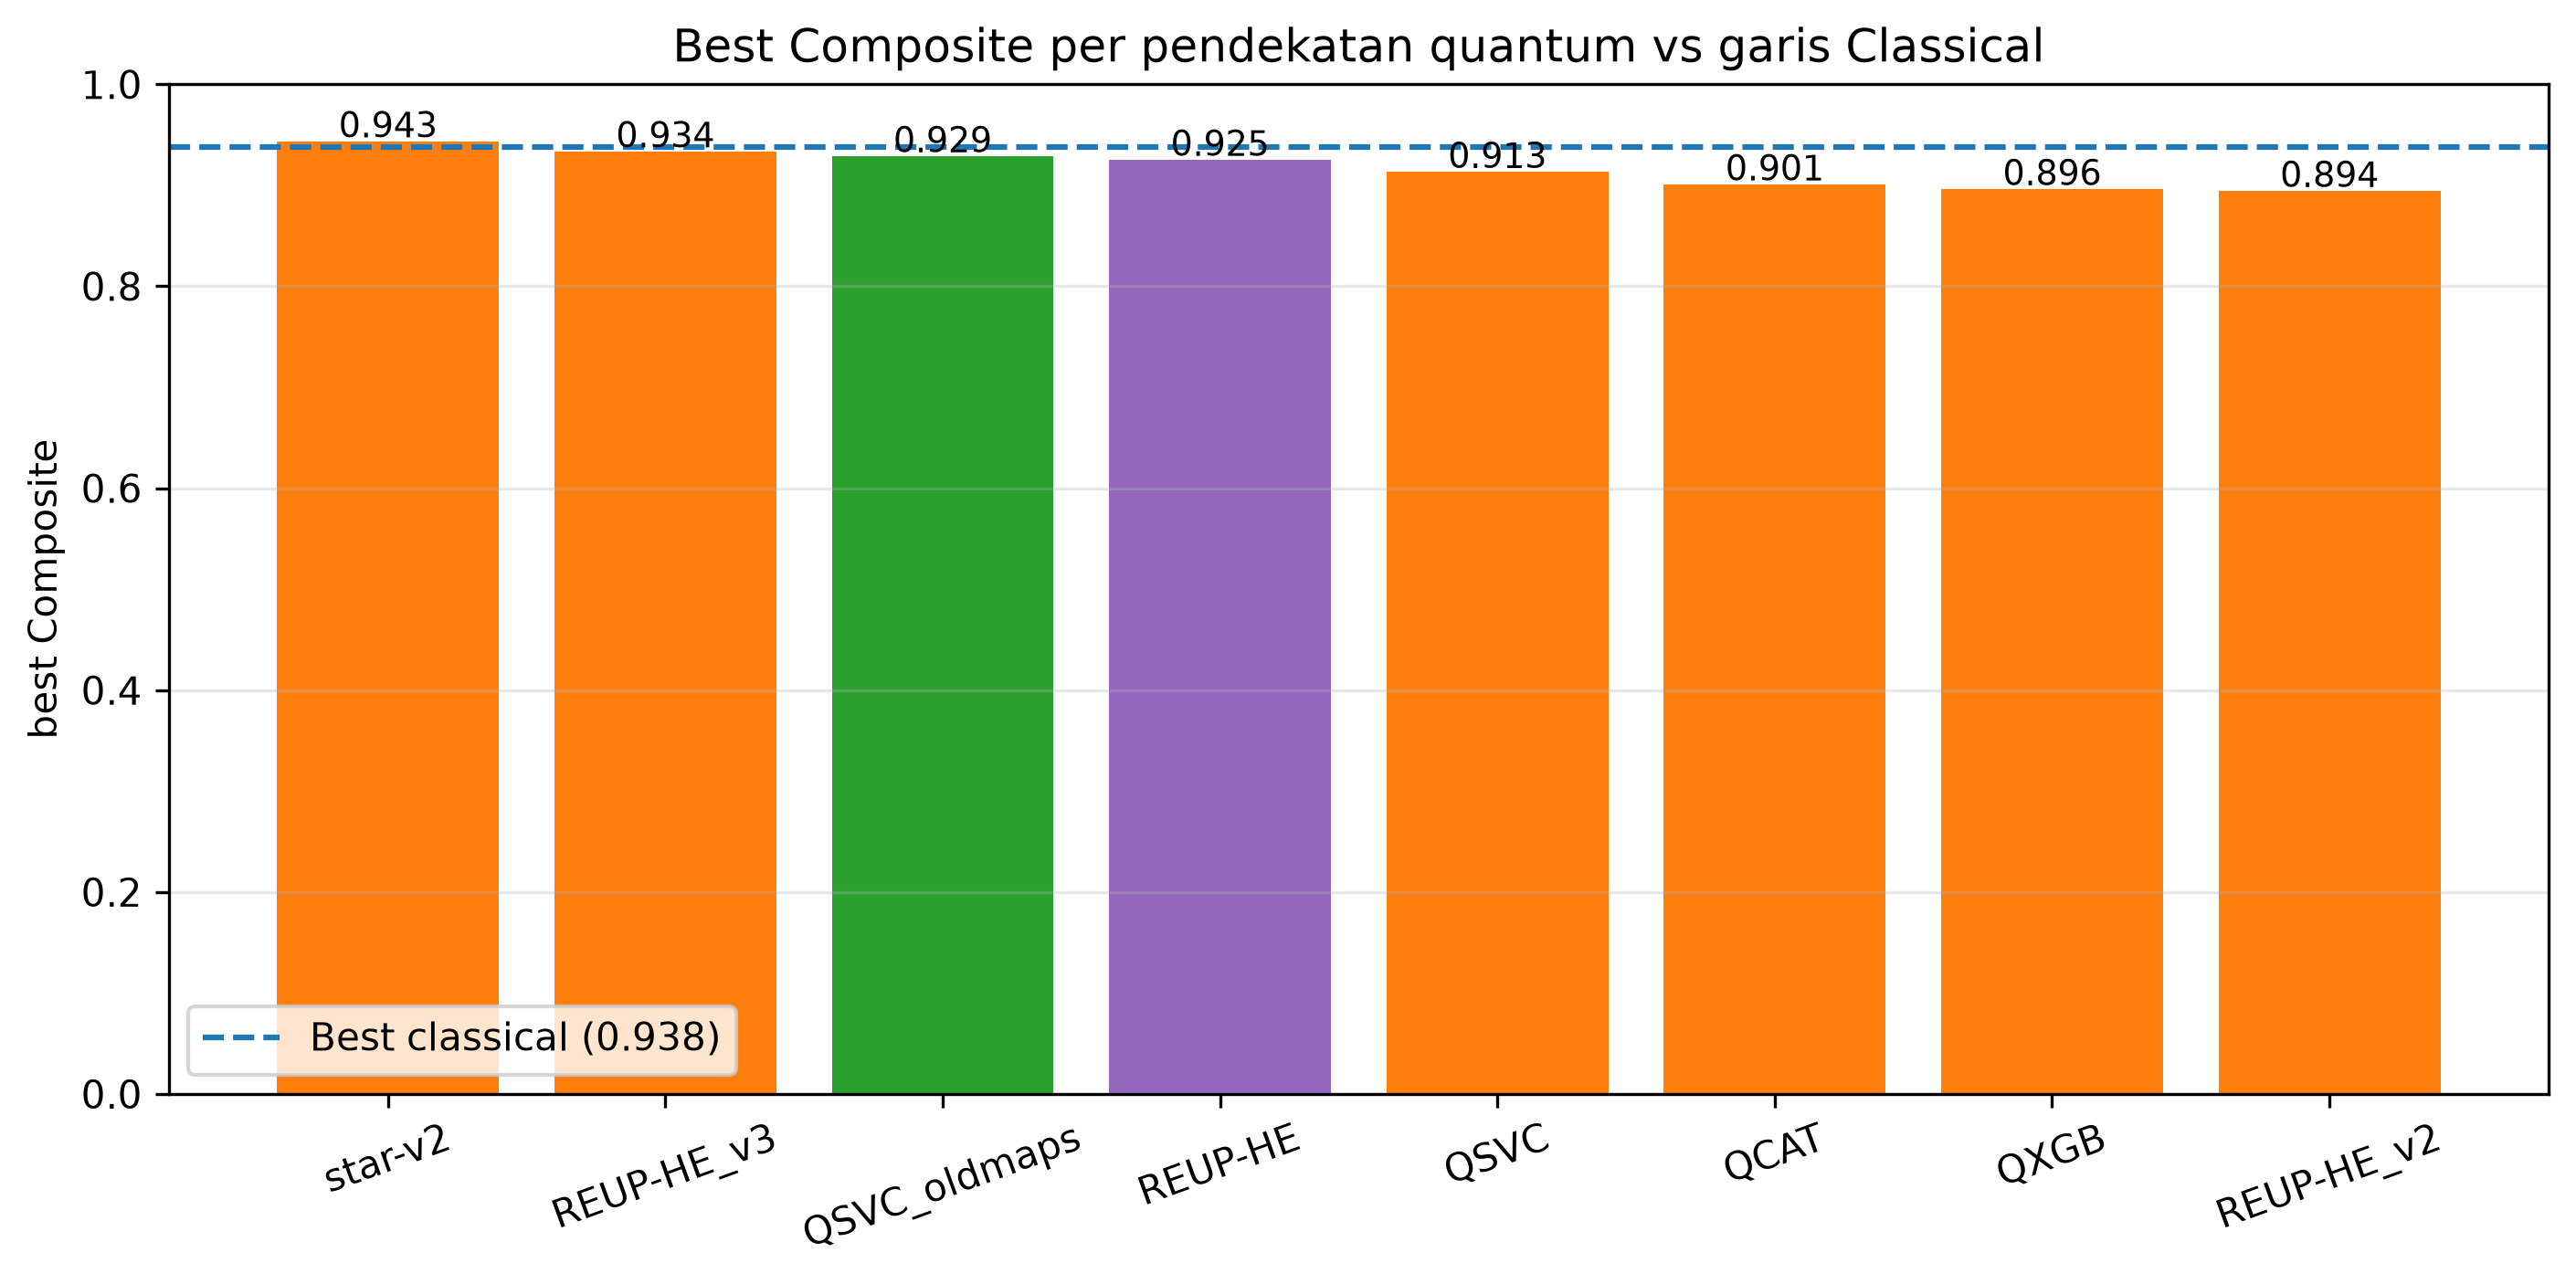
\includegraphics[width=\linewidth]{figure/qml/comparison/05_quantum_approaches.png}
\caption{Performance trajectory of various quantum approaches relative to the classical CatBoost baseline, highlighting the necessity of multi-basis encoding.}
\label{fig:quantum_approaches}
\end{figure}

The distinct performance gap between the \textit{star} map and the standard IQP baselines, visualized in Fig.~\ref{fig:quantum_approaches}, provides a critical diagnostic insight into the mechanics of the PQK. Standard IQP predominantly generates informative expectations on a single axis (the $Z$-basis), leaving the $\langle X \rangle$ and $\langle Y \rangle$ projection spaces virtually unutilized. Consequently, a substantial portion of the theoretical $3n$-dimensional feature space is wasted, effectively shrinking it to $n$. Conversely, the superior performance of the \textit{star} map proves that an active, multi-basis state-preparation layer significantly enhances the kernel's expressive power. This specific structural vulnerability in conventional IQP circuits serves as the precise theoretical motivation for formulating the proposed \textit{STAR-v2} feature map.

\subsubsection{The Proposed STAR-v2 Feature Map}

Building on this diagnosis, we formulate the proposed STAR-v2 feature map. STAR-v2 deliberately retains the lightweight single-hub (star) entanglement of the earlier \textit{star} map---identified above as the strongest baseline---but introduces three targeted modifications. First, the state preparation is enriched from a single-basis encoding ($H$, $R_Z$) to a multi-basis encoding ($H$, $R_Y(c\,x_i)$, $R_Z(c\,x_i)$), so that all three single-qubit Pauli expectations $\langle X\rangle$, $\langle Y\rangle$, and $\langle Z\rangle$ become informative and the wasted projection space identified above is reclaimed. Second, a fixed bandwidth $c=0.5$ is applied to every rotation angle to mitigate \textit{kernel concentration}, the regime in which all pairwise kernel values become nearly uniform and the kernel ceases to be discriminative. Third, the PQK bandwidth $\gamma$ is swept over $\{0.25,0.5\}$, widening the projected-space RBF to further counteract concentration. The entanglement structure is intentionally kept light (a single hub); denser, more expressive alternatives were found to be counterproductive, as detailed below.

Table \ref{tab:proposed_quantum} traces the design trajectory that led to STAR-v2 and confirms that raw expressivity is not the controlling factor for PQK performance. A re-uploading, hardware-efficient family (REUP-HE) was first explored. Its lightest variant (REUP-HE v1) improved recall over the IQP baseline but did not surpass the original \textit{star} map (0.9251 vs.\ 0.9287), and its densely entangled variant (REUP-HE v2) collapsed to 0.8943---direct empirical evidence that adding entanglement induces kernel concentration and degrades, rather than improves, PQK performance. The rotating-hub lite variant (REUP-HE v3) only recovered to 0.9280. The decisive gains instead came from controlling scale and encoding directly on the \textit{star} skeleton: simply lowering $\gamma$ raised \textit{star} from 0.9287 to 0.9335, and the full STAR-v2 redesign reached a Composite of \textbf{0.9435}---a $+0.0148$ improvement over the original \textit{star} and the highest Composite score recorded for any model in this study.

\begin{table}[htbp]
\caption{Design Evolution of the Proposed Quantum Feature Maps (QSVC, PCA = 12 qubits)}
\label{tab:proposed_quantum}
\centering
\resizebox{\columnwidth}{!}{
    \begin{tabular}{l c c c c c c}
    \hline
    \textbf{Feature Map} & \textbf{Acc} & \textbf{Recall} & \textbf{F1} & \textbf{MCC} & \textbf{PRAUC} & \textbf{Composite} \\
    \hline
    IQP-Full (baseline) & 0.9056 & 0.8298 & 0.8530 & 0.8646 & 0.9540 & 0.9131 \\
    star ($\gamma{=}1$) & 0.9091 & 0.8698 & 0.8869 & 0.8696 & 0.9643 & 0.9287 \\
    REUP-HE v1 & 0.9007 & 0.8680 & 0.8818 & 0.8578 & 0.9647 & 0.9251 \\
    REUP-HE v2 & 0.8495 & 0.8711 & 0.8535 & 0.7909 & 0.9338 & 0.8943 \\
    REUP-HE v3 & 0.9071 & 0.8759 & 0.8862 & 0.8673 & 0.9642 & 0.9280 \\
    star ($\gamma{=}0.5$) & 0.9113 & 0.8817 & 0.8924 & 0.8733 & 0.9714 & 0.9335 \\
    \textbf{STAR-v2} ($\gamma{=}0.5$) & \textbf{0.9179} & \textbf{0.9108} & \textbf{0.9110} & \textbf{0.8834} & \textbf{0.9777} & \textbf{0.9435} \\
    \hline
    \end{tabular}
}
\end{table}

The central narrative is therefore that the quantum advantage observed here does not arise from deeper circuits, more qubits, or heavier entanglement, but from \textit{aligning the feature map with the way the PQK operates}---activating multiple Pauli bases---combined with explicit scale control (bandwidth $c$ and a low $\gamma$) to keep the kernel from concentrating. This is a principled redesign rather than brute-force tuning: the optimization grid for STAR-v2 spans only the regularization parameter $C$ and the bandwidth $\gamma$.

To place the competing models on a common scale, Table \ref{tab:leaderboard} reports the Composite leaderboard across the three paradigms, listing only the best configuration of each model to keep the ranking compact. The table also exposes two instructive negative findings. The pure-phase encoding (\textit{$x$}-family, $R_X$ only) fails almost completely (Composite $\approx 0.252$, MCC $=0$), collapsing to a single-class prediction because it never activates the $\langle Z\rangle$ projection; and the densely entangled re-uploading variant (REUP-HE v2) drops to 0.80--0.89, confirming that excessive entanglement, not insufficient entanglement, is the failure mode for the PQK. These cases bracket the proposed STAR-v2 at the top of the ranking and substantiate the design philosophy of a multi-basis encoding with deliberately light entanglement.

\begin{table}[htbp]
\caption{Composite Leaderboard across Paradigms (best configuration per model; Q = Quantum, C = Classical, DL = Deep Learning)}
\label{tab:leaderboard}
\centering
\resizebox{\columnwidth}{!}{
    \begin{tabular}{c l l c c c c c c}
    \hline
    \textbf{\#} & \textbf{Par.} & \textbf{Model} & \textbf{Acc} & \textbf{F1} & \textbf{MCC} & \textbf{AUROC} & \textbf{PRAUC} & \textbf{Comp.} \\
    \hline
    1 & Q & \textbf{QSVC-STAR-v2} & 0.9179 & 0.9110 & 0.8834 & 0.9910 & 0.9777 & \textbf{0.9435} \\
    2 & DL & MLP & 0.9178 & 0.9025 & 0.8828 & 0.9924 & 0.9737 & 0.9392 \\
    3 & C & CatBoost & 0.9076 & 0.9124 & 0.8689 & 0.9895 & 0.9669 & 0.9379 \\
    4 & C & SVC-rbf & 0.9155 & 0.9068 & 0.8800 & 0.9916 & 0.9667 & 0.9378 \\
    5 & Q & QSVC-star ($\gamma{=}0.25$) & 0.9114 & 0.8953 & 0.8740 & 0.9903 & 0.9683 & 0.9336 \\
    6 & DL & 1D-CNN & 0.9058 & 0.8934 & 0.8672 & 0.9907 & 0.9651 & 0.9307 \\
    7 & Q & QSVC-reup\_lite & 0.9071 & 0.8862 & 0.8673 & 0.9901 & 0.9642 & 0.9280 \\
    8 & Q & QSVC-reup\_linear & 0.9007 & 0.8818 & 0.8578 & 0.9897 & 0.9647 & 0.9251 \\
    9 & C & XGBoost & 0.8979 & 0.8934 & 0.8544 & 0.9844 & 0.9519 & 0.9242 \\
    10 & Q & QSVC-IQP (full) & 0.9056 & 0.8530 & 0.8646 & 0.9901 & 0.9540 & 0.9131 \\
    11 & Q & QCAT-circular & 0.8830 & 0.8554 & 0.8339 & 0.9813 & 0.9299 & 0.9008 \\
    12 & Q & QXGB-full & 0.8816 & 0.8491 & 0.8300 & 0.9799 & 0.9241 & 0.8961 \\
    13 & Q & QSVC-reup\_ent\_full (v2) & 0.8495 & 0.8535 & 0.7909 & 0.9754 & 0.9338 & 0.8943 \\
    14 & C & SVC-poly & 0.8278 & 0.8229 & 0.7658 & 0.9591 & 0.8920 & 0.8659 \\
    -- & C & SVC-linear & 0.5378 & 0.5029 & 0.4020 & 0.8681 & 0.6203 & 0.6081 \\
    -- & C & SVC-sigmoid & 0.4755 & 0.4241 & 0.3467 & 0.8313 & 0.4946 & 0.5307 \\
    -- & Q & QSVC-$x$ ($R_X$ only) & 0.1730 & 0.0537 & 0.0000 & 0.5000 & 0.2024 & 0.2521 \\
    \hline
    \end{tabular}
}
\end{table}

\subsection{Comparison Between Classical and Quantum Models}

Table \ref{tab:three_way} contrasts the best model of each paradigm under the identical protocol. The proposed QSVC-STAR-v2 attains the highest Composite (0.9435), ahead of the best deep learning model (MLP, 0.9392) and the best classical model (CatBoost, 0.9379). The separating margins are small---0.0056 from quantum to deep learning and 0.0013 from deep learning to classical---and both lie well within the inter-fold standard deviation ($\approx 0.02$--$0.04$). The three leading models are thus most accurately described as a statistical tie at the top. Nonetheless, the nominal ranking is now led by the quantum kernel, which reverses the conventional expectation that classical methods dominate on tabular data and overturns the earlier baseline conclusion in which the classical models led.

\begin{table}[htbp]
\caption{Best Model per Paradigm under the Identical Protocol}
\label{tab:three_way}
\centering
\resizebox{\columnwidth}{!}{
    \begin{tabular}{l l c c c c c c c}
    \hline
    \textbf{Paradigm} & \textbf{Model} & \textbf{Acc} & \textbf{Prec} & \textbf{Recall} & \textbf{F1} & \textbf{MCC} & \textbf{AUROC} & \textbf{PRAUC} \\
    \hline
    \textbf{Quantum} & \textbf{QSVC-STAR-v2} & \textbf{0.9179} & 0.9220 & 0.9108 & 0.9110 & \textbf{0.8834} & 0.9910 & \textbf{0.9777} \\
    Deep Learning & MLP & 0.9178 & \textbf{0.9228} & 0.8980 & 0.9025 & 0.8828 & \textbf{0.9924} & 0.9737 \\
    Classical & CatBoost & 0.9076 & 0.9135 & \textbf{0.9172} & \textbf{0.9124} & 0.8689 & 0.9895 & 0.9669 \\
    \hline
    \multicolumn{9}{l}{\footnotesize Composite: QSVC-STAR-v2 = \textbf{0.9435}, MLP = 0.9392, CatBoost = 0.9379.} \\
    \end{tabular}
}
\end{table}

\begin{figure}[htbp]
\centering
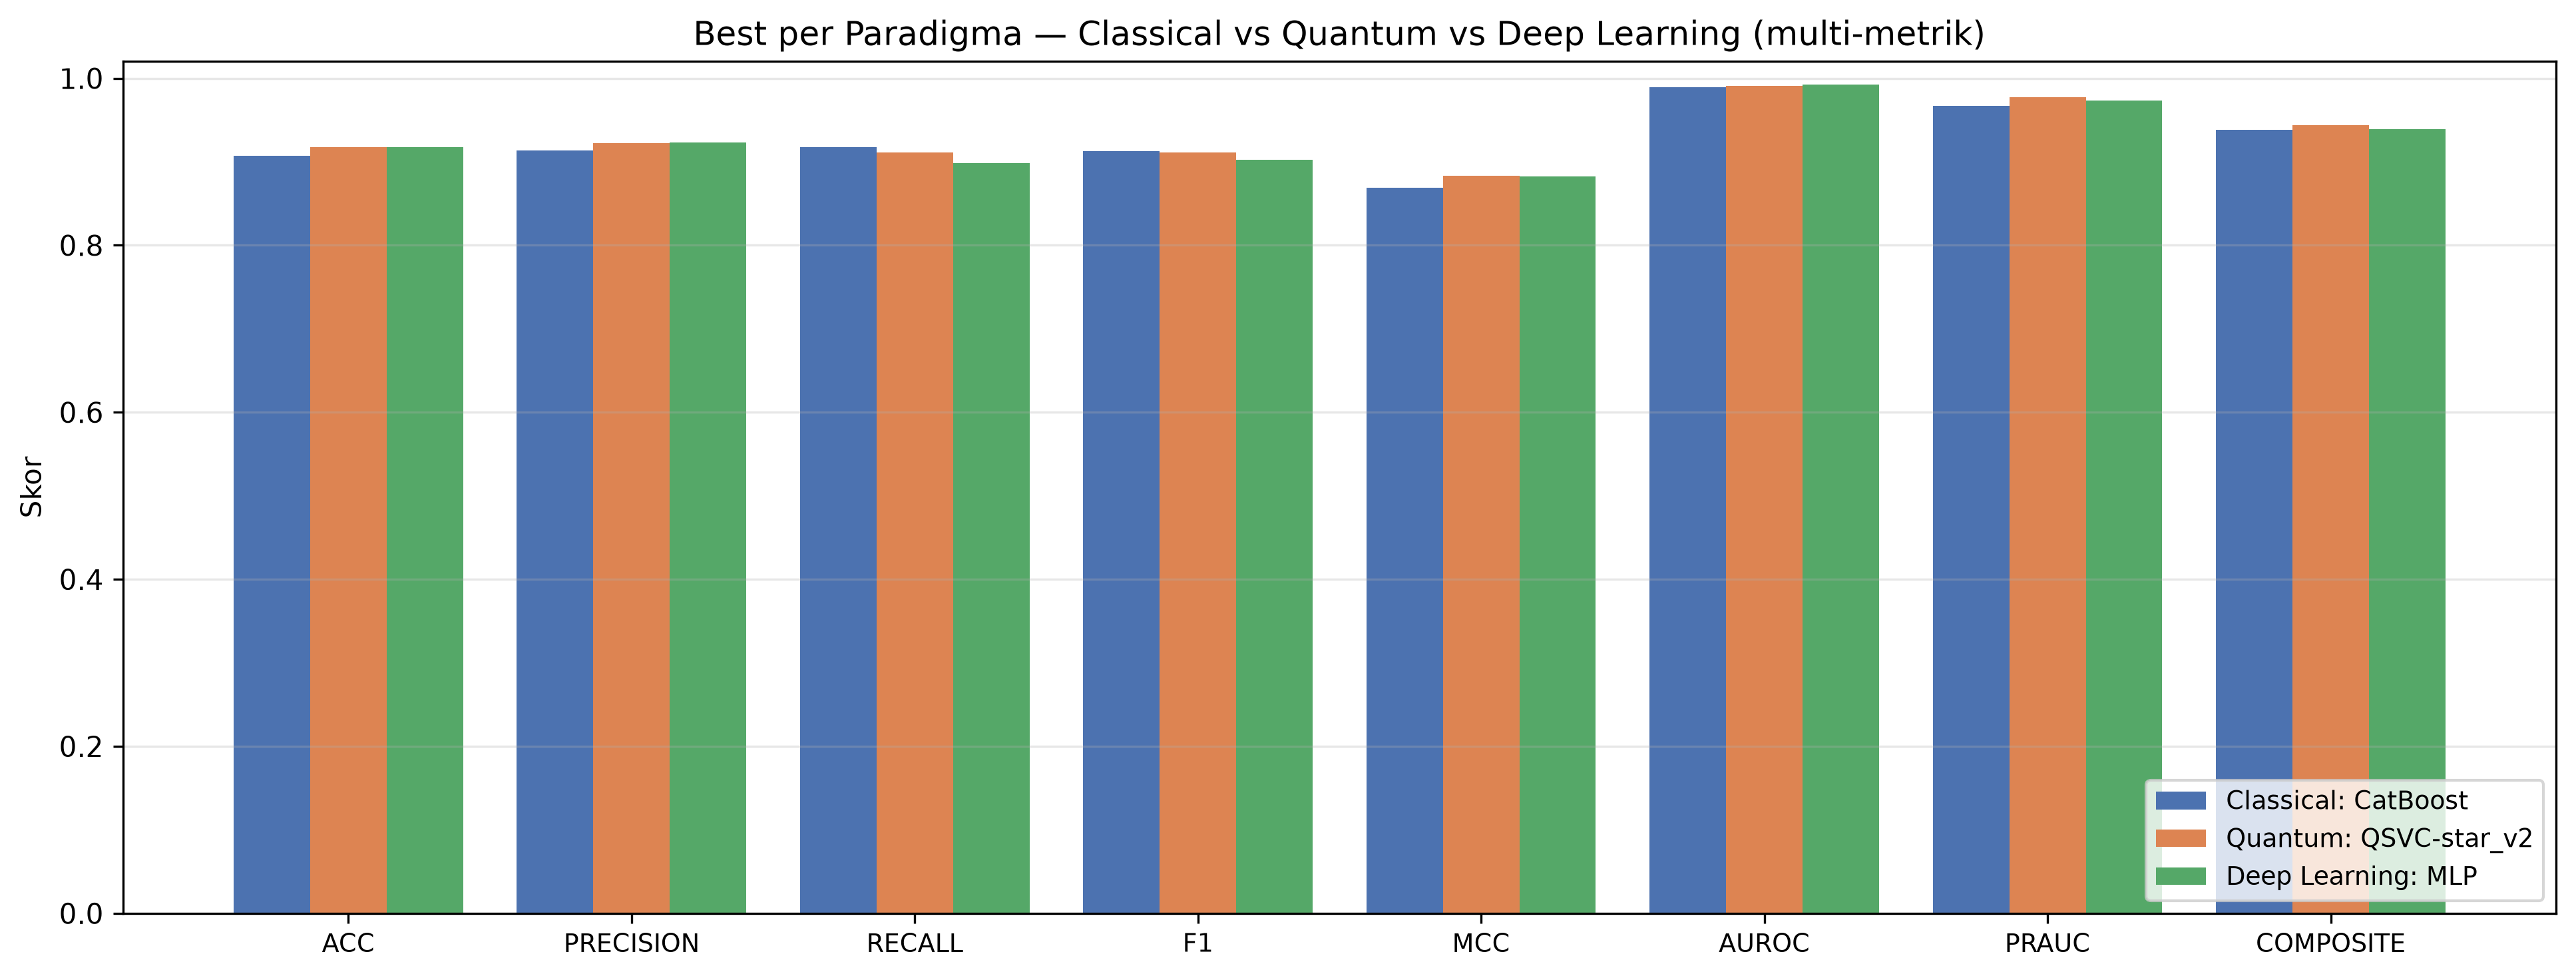
\includegraphics[width=\linewidth]{figure/qml/comparison/07_best_three_way.png}
\caption{Multi-metric comparison of the best model per paradigm (Classical vs.\ Quantum vs.\ Deep Learning), illustrating that each paradigm leads a distinct performance profile.}
\label{fig:three_way}
\end{figure}

Critically, no single paradigm dominates every metric; each leads a distinct performance profile, as visualized in Fig.~\ref{fig:three_way} and itemized metric-by-metric in Table \ref{tab:per_metric_winner}. The quantum kernel leads on Accuracy, MCC, PRAUC, and the Composite; the deep learning model leads on Precision and AUROC; and the classical model leads on Recall and macro-F1. The most consequential of these is the quantum advantage on PRAUC (0.9777), the metric most sensitive to minority classes, which directly addresses the central challenge of the imbalanced dataset.

\begin{table}[htbp]
\caption{Per-Metric Winner across the Three Paradigms}
\label{tab:per_metric_winner}
\centering
\resizebox{\columnwidth}{!}{
    \begin{tabular}{l c c c l}
    \hline
    \textbf{Metric} & \textbf{Classical} & \textbf{Quantum} & \textbf{DL} & \textbf{Winner} \\
     & \textbf{(CatBoost)} & \textbf{(STAR-v2)} & \textbf{(MLP)} & \\
    \hline
    Accuracy & 0.9076 & \textbf{0.9179} & 0.9178 & Quantum \\
    Precision & 0.9135 & 0.9220 & \textbf{0.9228} & DL \\
    Recall & \textbf{0.9172} & 0.9108 & 0.8980 & Classical \\
    macro-F1 & \textbf{0.9124} & 0.9110 & 0.9025 & Classical \\
    MCC & 0.8689 & \textbf{0.8834} & 0.8828 & Quantum \\
    AUROC & 0.9895 & 0.9910 & \textbf{0.9924} & DL \\
    PRAUC & 0.9669 & \textbf{0.9777} & 0.9737 & Quantum \\
    Composite & 0.9379 & \textbf{0.9435} & 0.9392 & Quantum \\
    \hline
    \end{tabular}
}
\end{table}

The head-to-head profile of the best classical and best quantum models is shown in Fig.~\ref{fig:best_cq}, and the signed per-metric difference ($\Delta = $ quantum $-$ classical) in Fig.~\ref{fig:delta_cq}. The quantum kernel posts its largest positive margins exactly on the minority-sensitive metrics (PRAUC and MCC), while conceding only marginally on recall---a balanced trade that nonetheless places it ahead on the aggregate Composite.

\begin{figure}[htbp]
\centering
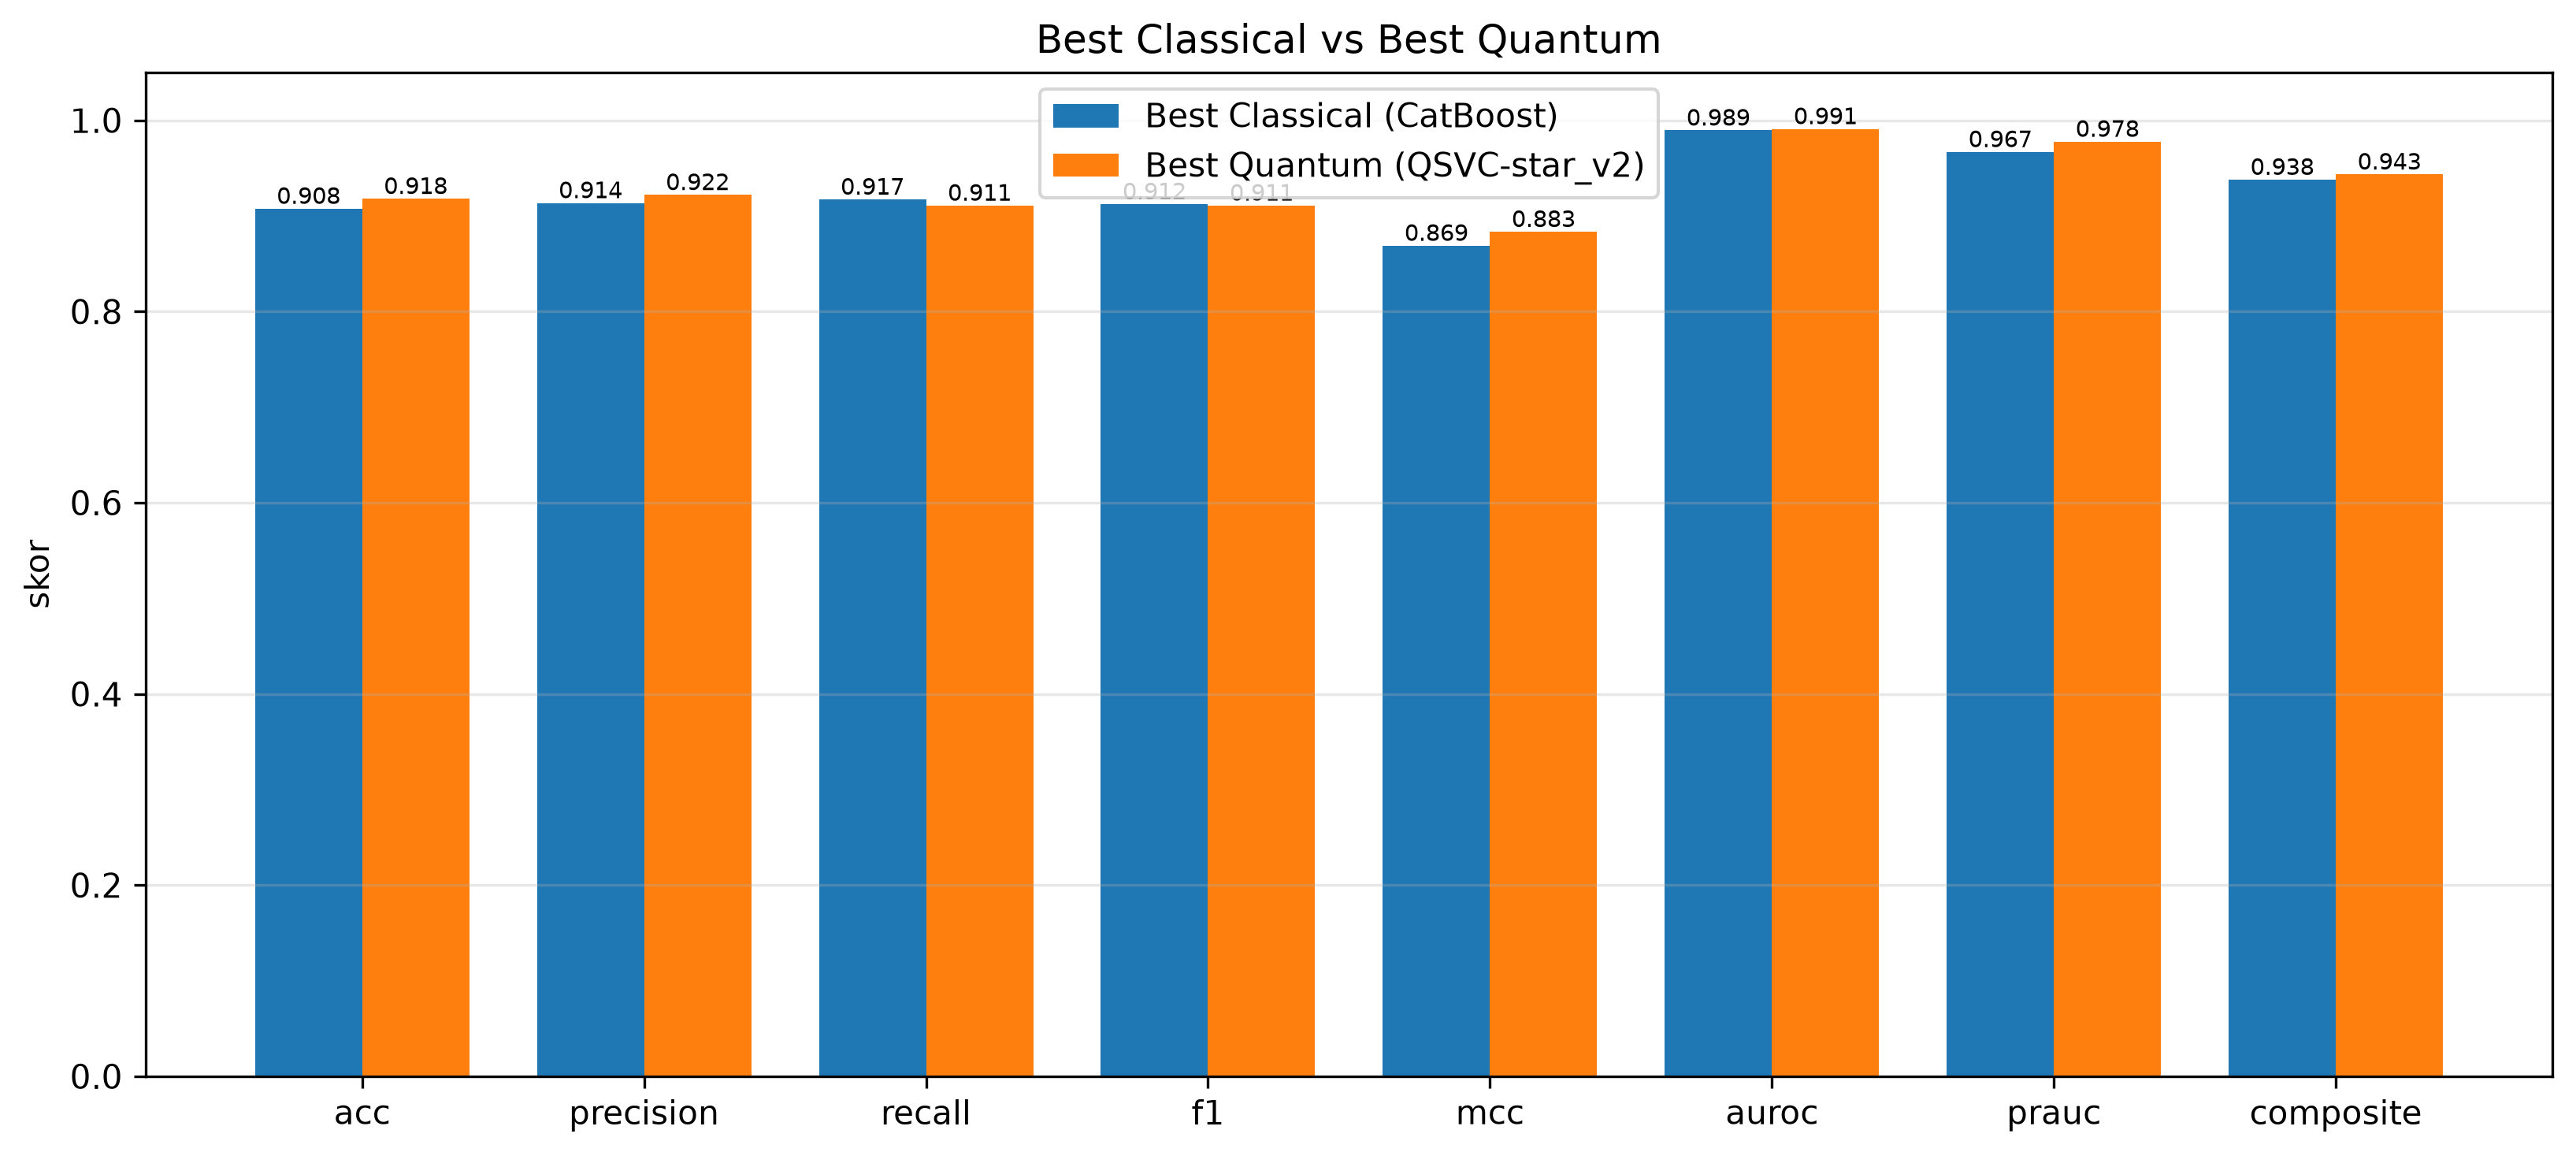
\includegraphics[width=\linewidth]{figure/qml/comparison/01_best_classical_vs_quantum.png}
\caption{Best classical (CatBoost) versus best quantum (STAR-v2) model across all reported metrics.}
\label{fig:best_cq}
\end{figure}

\begin{figure}[htbp]
\centering
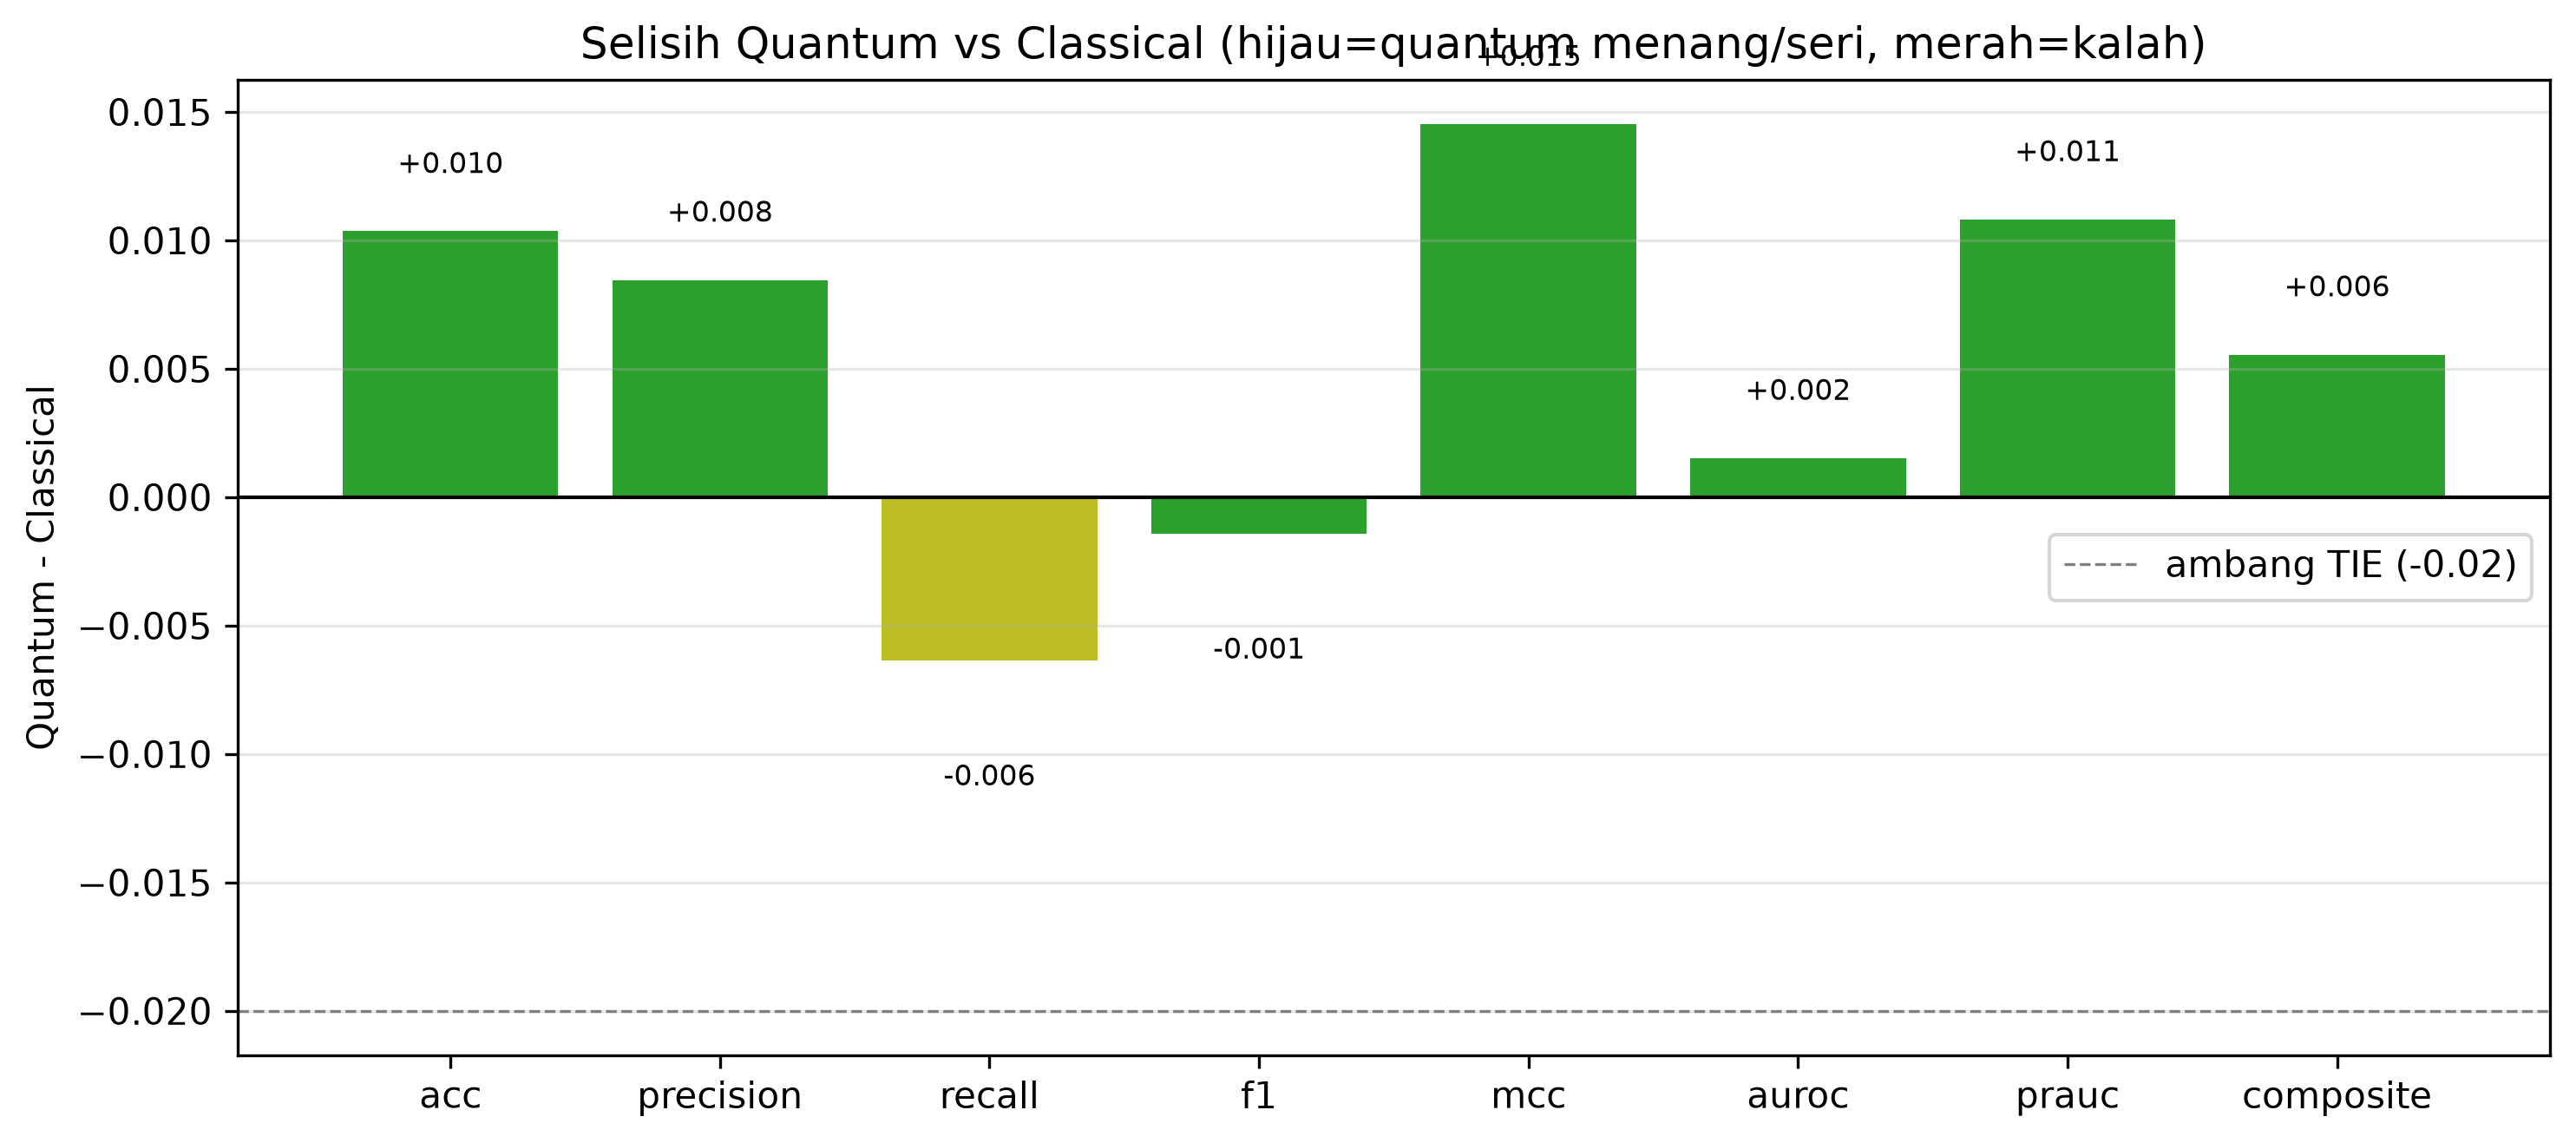
\includegraphics[width=\linewidth]{figure/qml/comparison/03_delta_quantum_vs_classical.png}
\caption{Signed per-metric difference between the best quantum and best classical models; positive values favor the quantum kernel, with the largest gains on PRAUC and MCC.}
\label{fig:delta_cq}
\end{figure}

A paired, family-wise comparison (Table \ref{tab:paired_family} and Fig.~\ref{fig:paired_family}) clarifies where the quantum models are genuinely competitive. Within the kernel/SVM family, the quantum model now \textit{surpasses} its classical counterpart on almost every metric (QSVC-STAR-v2 0.9435 vs.\ SVC-rbf 0.9378; $\Delta$Composite $=+0.0056$, $\Delta$PRAUC $=+0.011$, $\Delta$Precision $=+0.0168$)---an unsurprising outcome given that the ``quantum'' component is itself a kernel. By contrast, the hybrid tree families remain behind their classical equivalents (QCAT-Circular 0.9008 vs.\ CatBoost 0.9379; QXGB-Full 0.8961 vs.\ XGBoost 0.9242), reaffirming that the quantum kernel is most effective when used directly as an SVM kernel rather than reduced to input features for a classical tree.

\begin{table}[htbp]
\caption{Paired Family-wise Comparison of Composite Scores}
\label{tab:paired_family}
\centering
\resizebox{\columnwidth}{!}{
    \begin{tabular}{l l c l c c}
    \hline
    \textbf{Family} & \textbf{Classical} & \textbf{Comp.} & \textbf{Quantum} & \textbf{Comp.} & \textbf{Gain (Q-C)} \\
    \hline
    Kernel / SVM & SVC-rbf & 0.9378 & QSVC-STAR-v2 & \textbf{0.9435} & \textbf{+0.0056} \\
    Boosting (Cat) & CatBoost & 0.9379 & QCAT-circular & 0.9008 & $-0.0371$ \\
    Boosting (XGB) & XGBoost & 0.9242 & QXGB-full & 0.8961 & $-0.0281$ \\
    \hline
    \end{tabular}
}
\end{table}

\begin{figure}[htbp]
\centering
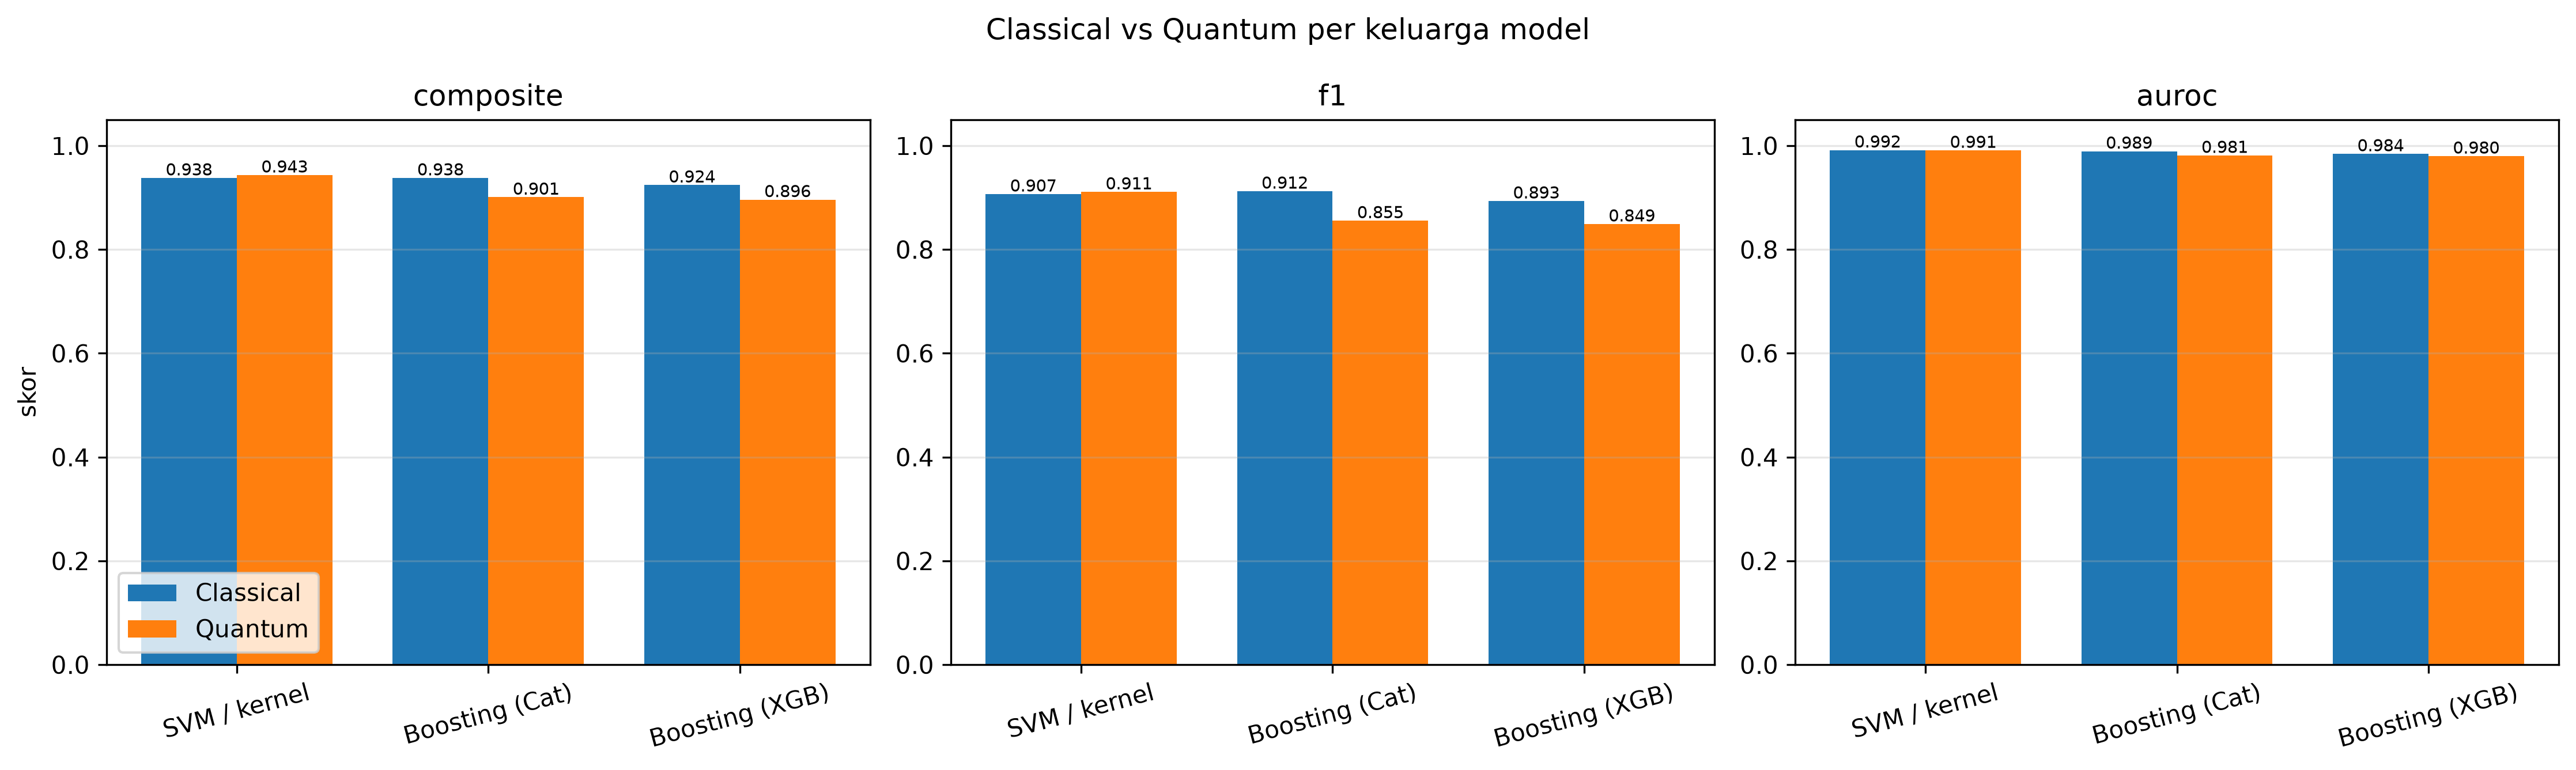
\includegraphics[width=\linewidth]{figure/qml/comparison/02_paired_family.png}
\caption{Family-wise comparison of classical and quantum models, showing the quantum advantage confined to the kernel/SVM family.}
\label{fig:paired_family}
\end{figure}

Table \ref{tab:per_pca} examines performance as a function of the PCA dimension, which equals the number of qubits for the quantum models. The long-standing hypothesis that quantum methods would be most advantageous at low dimensionality is not supported: the quantum kernel is in fact \textit{stronger with more qubits}, because a sufficient number of qubits is needed to encode the interactions among the 12 sensor features. At PCA $=8$ and PCA $=12$, STAR-v2 outperforms the best classical model, whereas at PCA $=3$ the two are essentially tied; deep learning provides the best non-classical result at PCA $=5$. This trend is depicted in Fig.~\ref{fig:per_pca}.

\begin{table}[htbp]
\caption{Best Classical vs.\ Best Non-Classical Model per PCA Dimension (Composite)}
\label{tab:per_pca}
\centering
\resizebox{\columnwidth}{!}{
    \begin{tabular}{c l c l c c}
    \hline
    \textbf{PCA} & \textbf{Classical} & \textbf{Comp.} & \textbf{Non-Classical} & \textbf{Comp.} & \textbf{Winner} \\
    \hline
    3 & CatBoost & 0.7782 & QSVC-STAR-v2 & 0.7779 & Classical \\
    5 & SVC-rbf & 0.8983 & MLP & 0.9100 & Deep Learning \\
    8 & SVC-rbf & 0.9323 & QSVC-STAR-v2 & 0.9376 & \textbf{Quantum} \\
    12 & CatBoost & 0.9379 & QSVC-STAR-v2 & 0.9435 & \textbf{Quantum} \\
    \hline
    \end{tabular}
}
\end{table}

\begin{figure}[htbp]
\centering
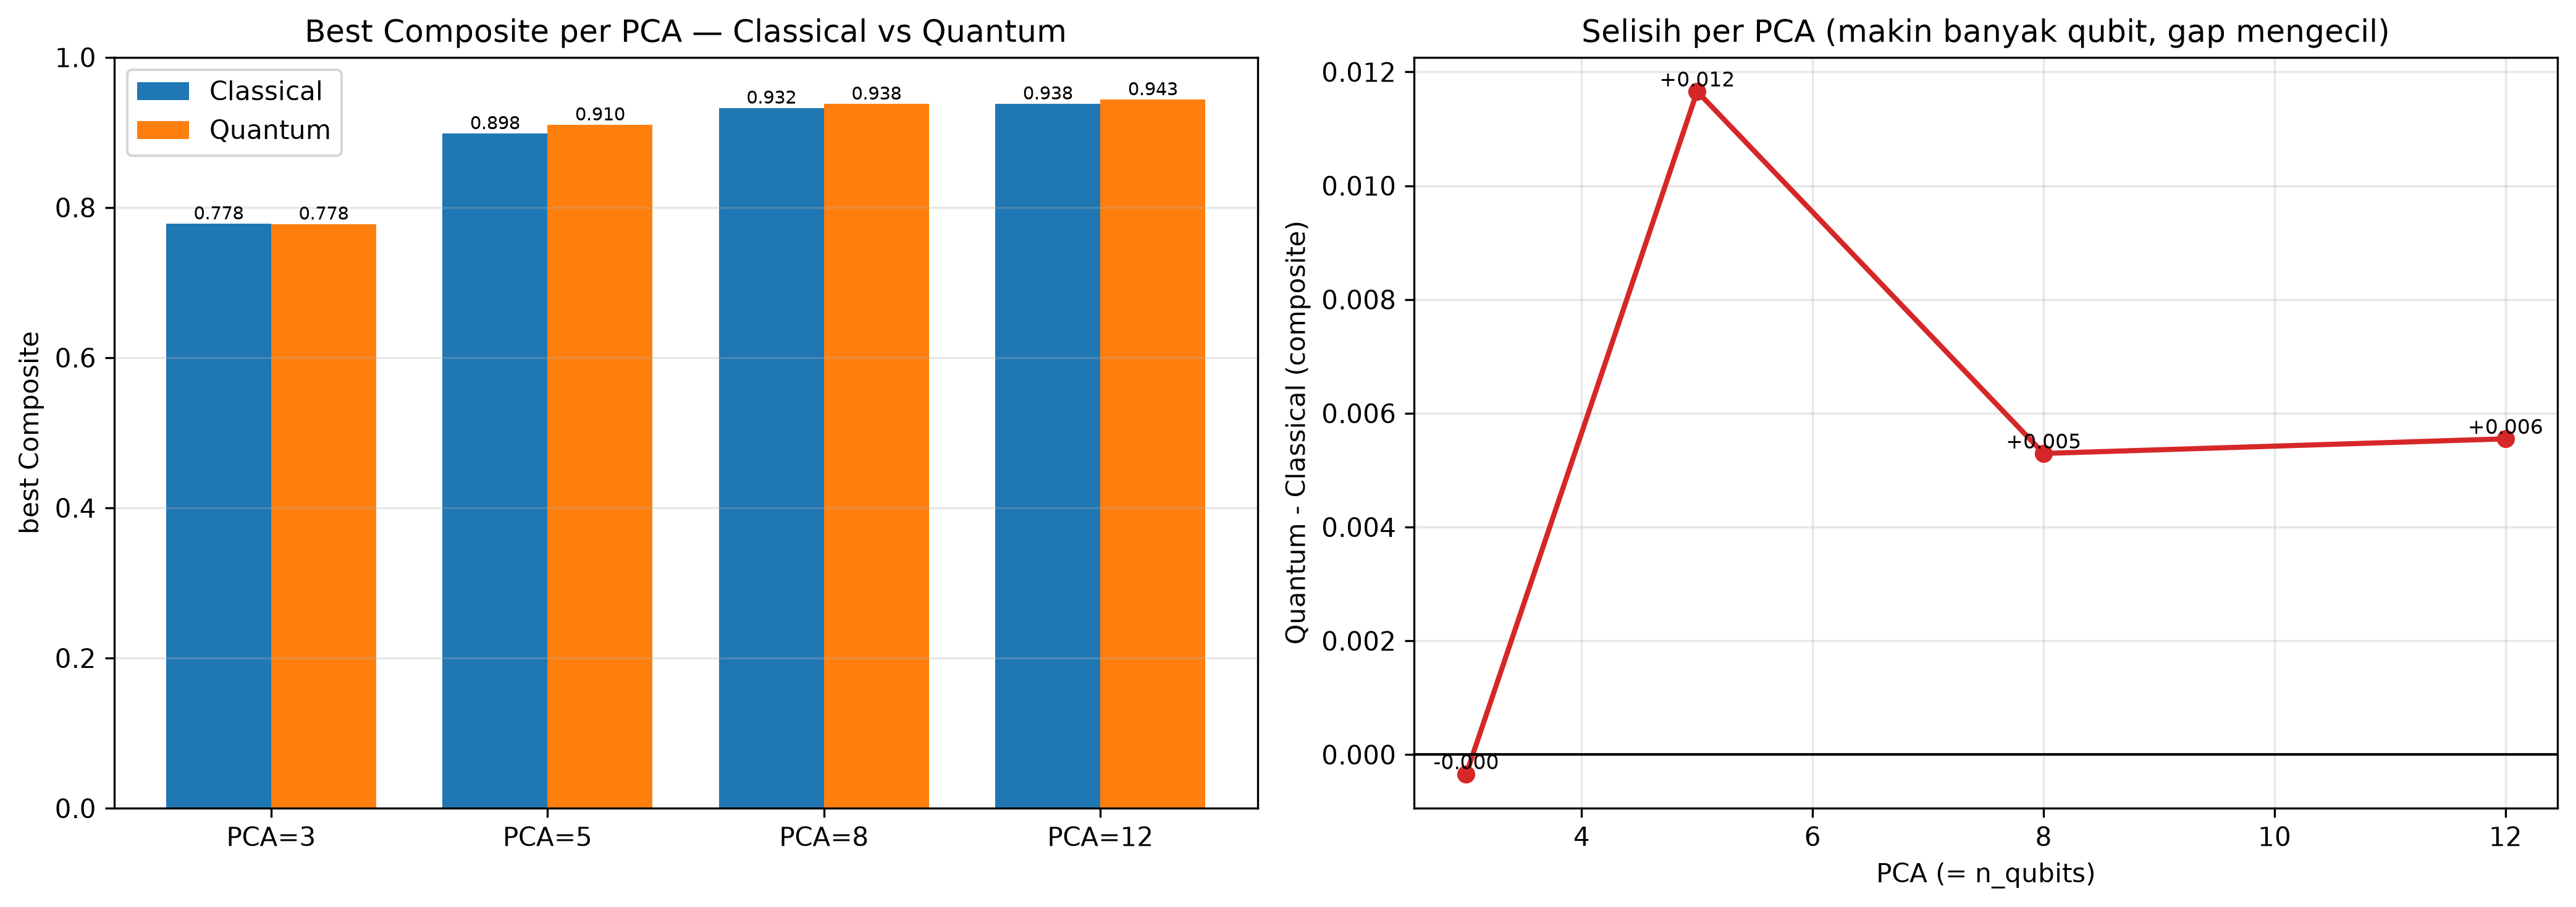
\includegraphics[width=\linewidth]{figure/qml/comparison/04_per_pca_classical_vs_quantum.png}
\caption{Composite score of the best classical and best non-classical models as a function of the PCA dimension (number of qubits), showing that the quantum kernel becomes competitive and then superior as the qubit count grows.}
\label{fig:per_pca}
\end{figure}

\subsection{Class Level Performance and Minority Class Handling}

To understand the source of the quantum advantage, Table \ref{tab:per_class} reports the per-class recall and F1 of STAR-v2 (obtained from out-of-fold predictions) alongside the recall of the original \textit{star} map. The improvements are concentrated precisely where the dataset is most difficult: on the rarest class B, recall increases by $+0.118$ (from 0.755 to 0.873), and on class C by $+0.038$. These gains are a direct consequence of the multi-basis encoding and bandwidth control, which activate the Pauli features that the single-basis baseline had wasted. Notably, despite being the rarest grade (only 2.2\% of rows), class B is in fact among the easiest to recognize, reaching an F1 of 0.928---most plausibly because its chemistry is the most distinct.

\begin{table}[htbp]
\caption{Per-Class Recall and F1 of STAR-v2 (Out-of-Fold) vs.\ the Original \textit{star} Map}
\label{tab:per_class}
\centering
\resizebox{\columnwidth}{!}{
    \begin{tabular}{c c c c c}
    \hline
    \textbf{Class} & \textbf{STAR-v2 Recall} & \textbf{STAR-v2 F1} & \textbf{star Recall} & \textbf{Recall Gain} \\
    \hline
    A & 0.924 & 0.891 & 0.918 & $+0.006$ \\
    \textbf{B} (minority) & \textbf{0.873} & \textbf{0.928} & 0.755 & \textbf{+0.118} \\
    C & 0.955 & 0.946 & 0.917 & $+0.038$ \\
    D (hardest) & 0.876 & 0.860 & 0.874 & $+0.002$ \\
    E & 0.921 & 0.939 & 0.934 & $-0.013$ \\
    \hline
    \end{tabular}
}
\end{table}

The confusion structure, shown in Fig.~\ref{fig:starv2_confusion}, identifies grade D as the persistently hardest class (recall 0.876), confused chiefly with its neighboring grades A ($\approx 4.4\%$) and E ($\approx 4.6\%$). This is the same error pattern observed in the classical and deep learning models, which indicates that classification difficulty is driven by chemical similarity between adjacent quality grades (A--D--E) rather than by class rarity. The robustness of this pattern across all three paradigms confirms it to be a property of the dataset itself, not an artifact of any single model. The class-wise ROC and Precision--Recall curves in Fig.~\ref{fig:starv2_roc_pr} corroborate this view, with D exhibiting the lowest area under the curve and B among the highest despite its scarcity.

\begin{figure}[htbp]
\centering

\includegraphics[width=\linewidth]{figure/qml/star-v2/10_confusion_matrix.png}
\caption{Normalized out-of-fold confusion matrix of the proposed STAR-v2 model, showing grade D as the dominant source of error (confused with adjacent grades A and E).}
\label{fig:starv2_confusion}
\end{figure}

\begin{figure}[htbp]
\centering

\includegraphics[width=\linewidth]{figure/qml/star-v2/12_roc_pr_ovr.png}
\caption{One-vs-rest ROC and Precision--Recall curves of STAR-v2, confirming strong separability for the minority grade B and the comparative difficulty of grade D.}
\label{fig:starv2_roc_pr}
\end{figure}

The per-class F1 of STAR-v2 is mapped in Fig.~\ref{fig:starv2_f1class}, and Table \ref{tab:per_class_cross} compares the per-class recall of the best model from each paradigm. The agreement is striking: grade D is the weakest class for every paradigm and grade B is among the strongest despite being the rarest, which establishes that the difficulty structure is intrinsic to the e-nose chemistry rather than an artifact of a particular model family. The only notable divergence is that the classical CatBoost achieves a perfect recall on B, whereas the quantum and deep learning models trade a small amount of B-recall for higher recall elsewhere.

\begin{table}[htbp]
\caption{Per-Class Recall of the Best Model per Paradigm (Out-of-Fold)}
\label{tab:per_class_cross}
\centering
\resizebox{\columnwidth}{!}{
    \begin{tabular}{c c c c}
    \hline
    \textbf{Class} & \textbf{Classical} & \textbf{Quantum} & \textbf{DL} \\
     & \textbf{(CatBoost)} & \textbf{(STAR-v2)} & \textbf{(MLP)} \\
    \hline
    A & 0.89 & 0.924 & 0.902 \\
    \textbf{B} (minority) & \textbf{1.00} & 0.873 & 0.843 \\
    C & 0.92 & 0.955 & 0.920 \\
    \textbf{D} (hardest) & 0.86 & 0.876 & 0.879 \\
    E & 0.92 & 0.921 & 0.943 \\
    \hline
    \end{tabular}
}
\end{table}

\begin{figure}[htbp]
\centering

\includegraphics[width=\linewidth]{figure/qml/star-v2/11_f1_per_kelas_heatmap.png}
\caption{Per-class F1 heatmap of STAR-v2, highlighting the recovered performance on the minority grade B and the residual weakness on grade D.}
\label{fig:starv2_f1class}
\end{figure}

For completeness, the same class-level diagnostics are reported for the strongest classical and deep learning models. Fig.~\ref{fig:classical_confusion} shows the per-model classical confusion matrices and Fig.~\ref{fig:classical_roc_pr} the corresponding ROC and Precision--Recall curves, while Fig.~\ref{fig:dl_confusion} shows the deep learning confusion matrices. In all cases the off-diagonal mass concentrates along the A--D--E band, reproducing the same adjacency-driven error structure and confirming that the Precision--Recall view is more honest than ROC under this degree of imbalance.

\begin{figure}[htbp]
\centering
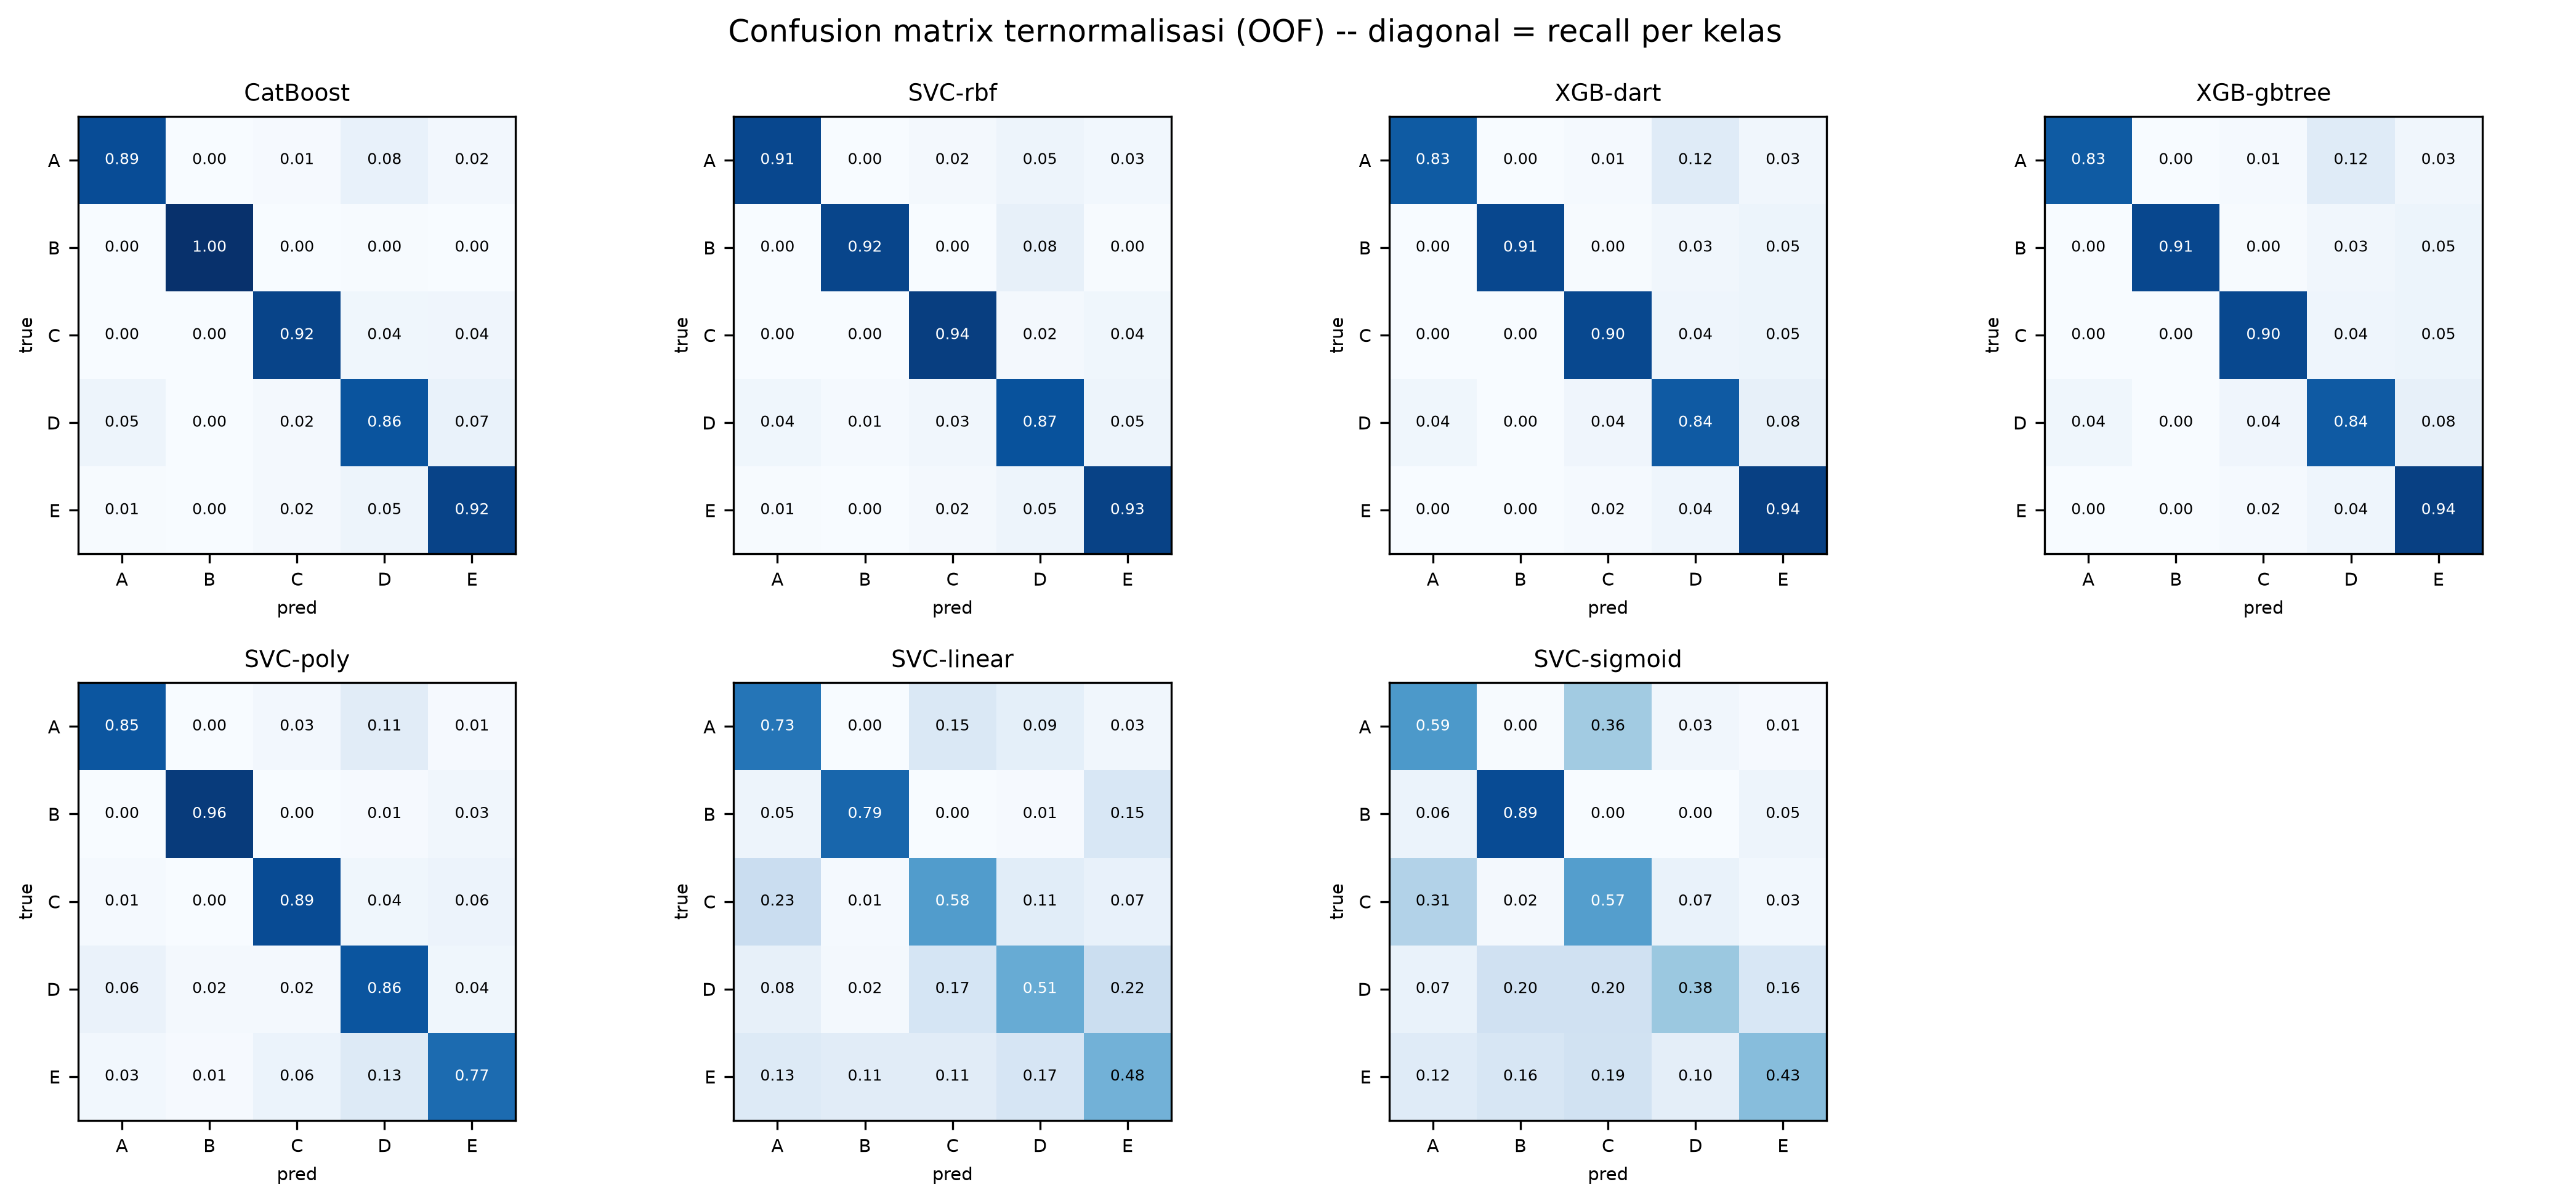
\includegraphics[width=\linewidth]{figure/out-new/10_confusion_matrix.png}
\caption{Normalized out-of-fold confusion matrices of the classical models; the diagonal equals per-class recall, and grade D is the dominant source of confusion.}
\label{fig:classical_confusion}
\end{figure}

\begin{figure}[htbp]
\centering
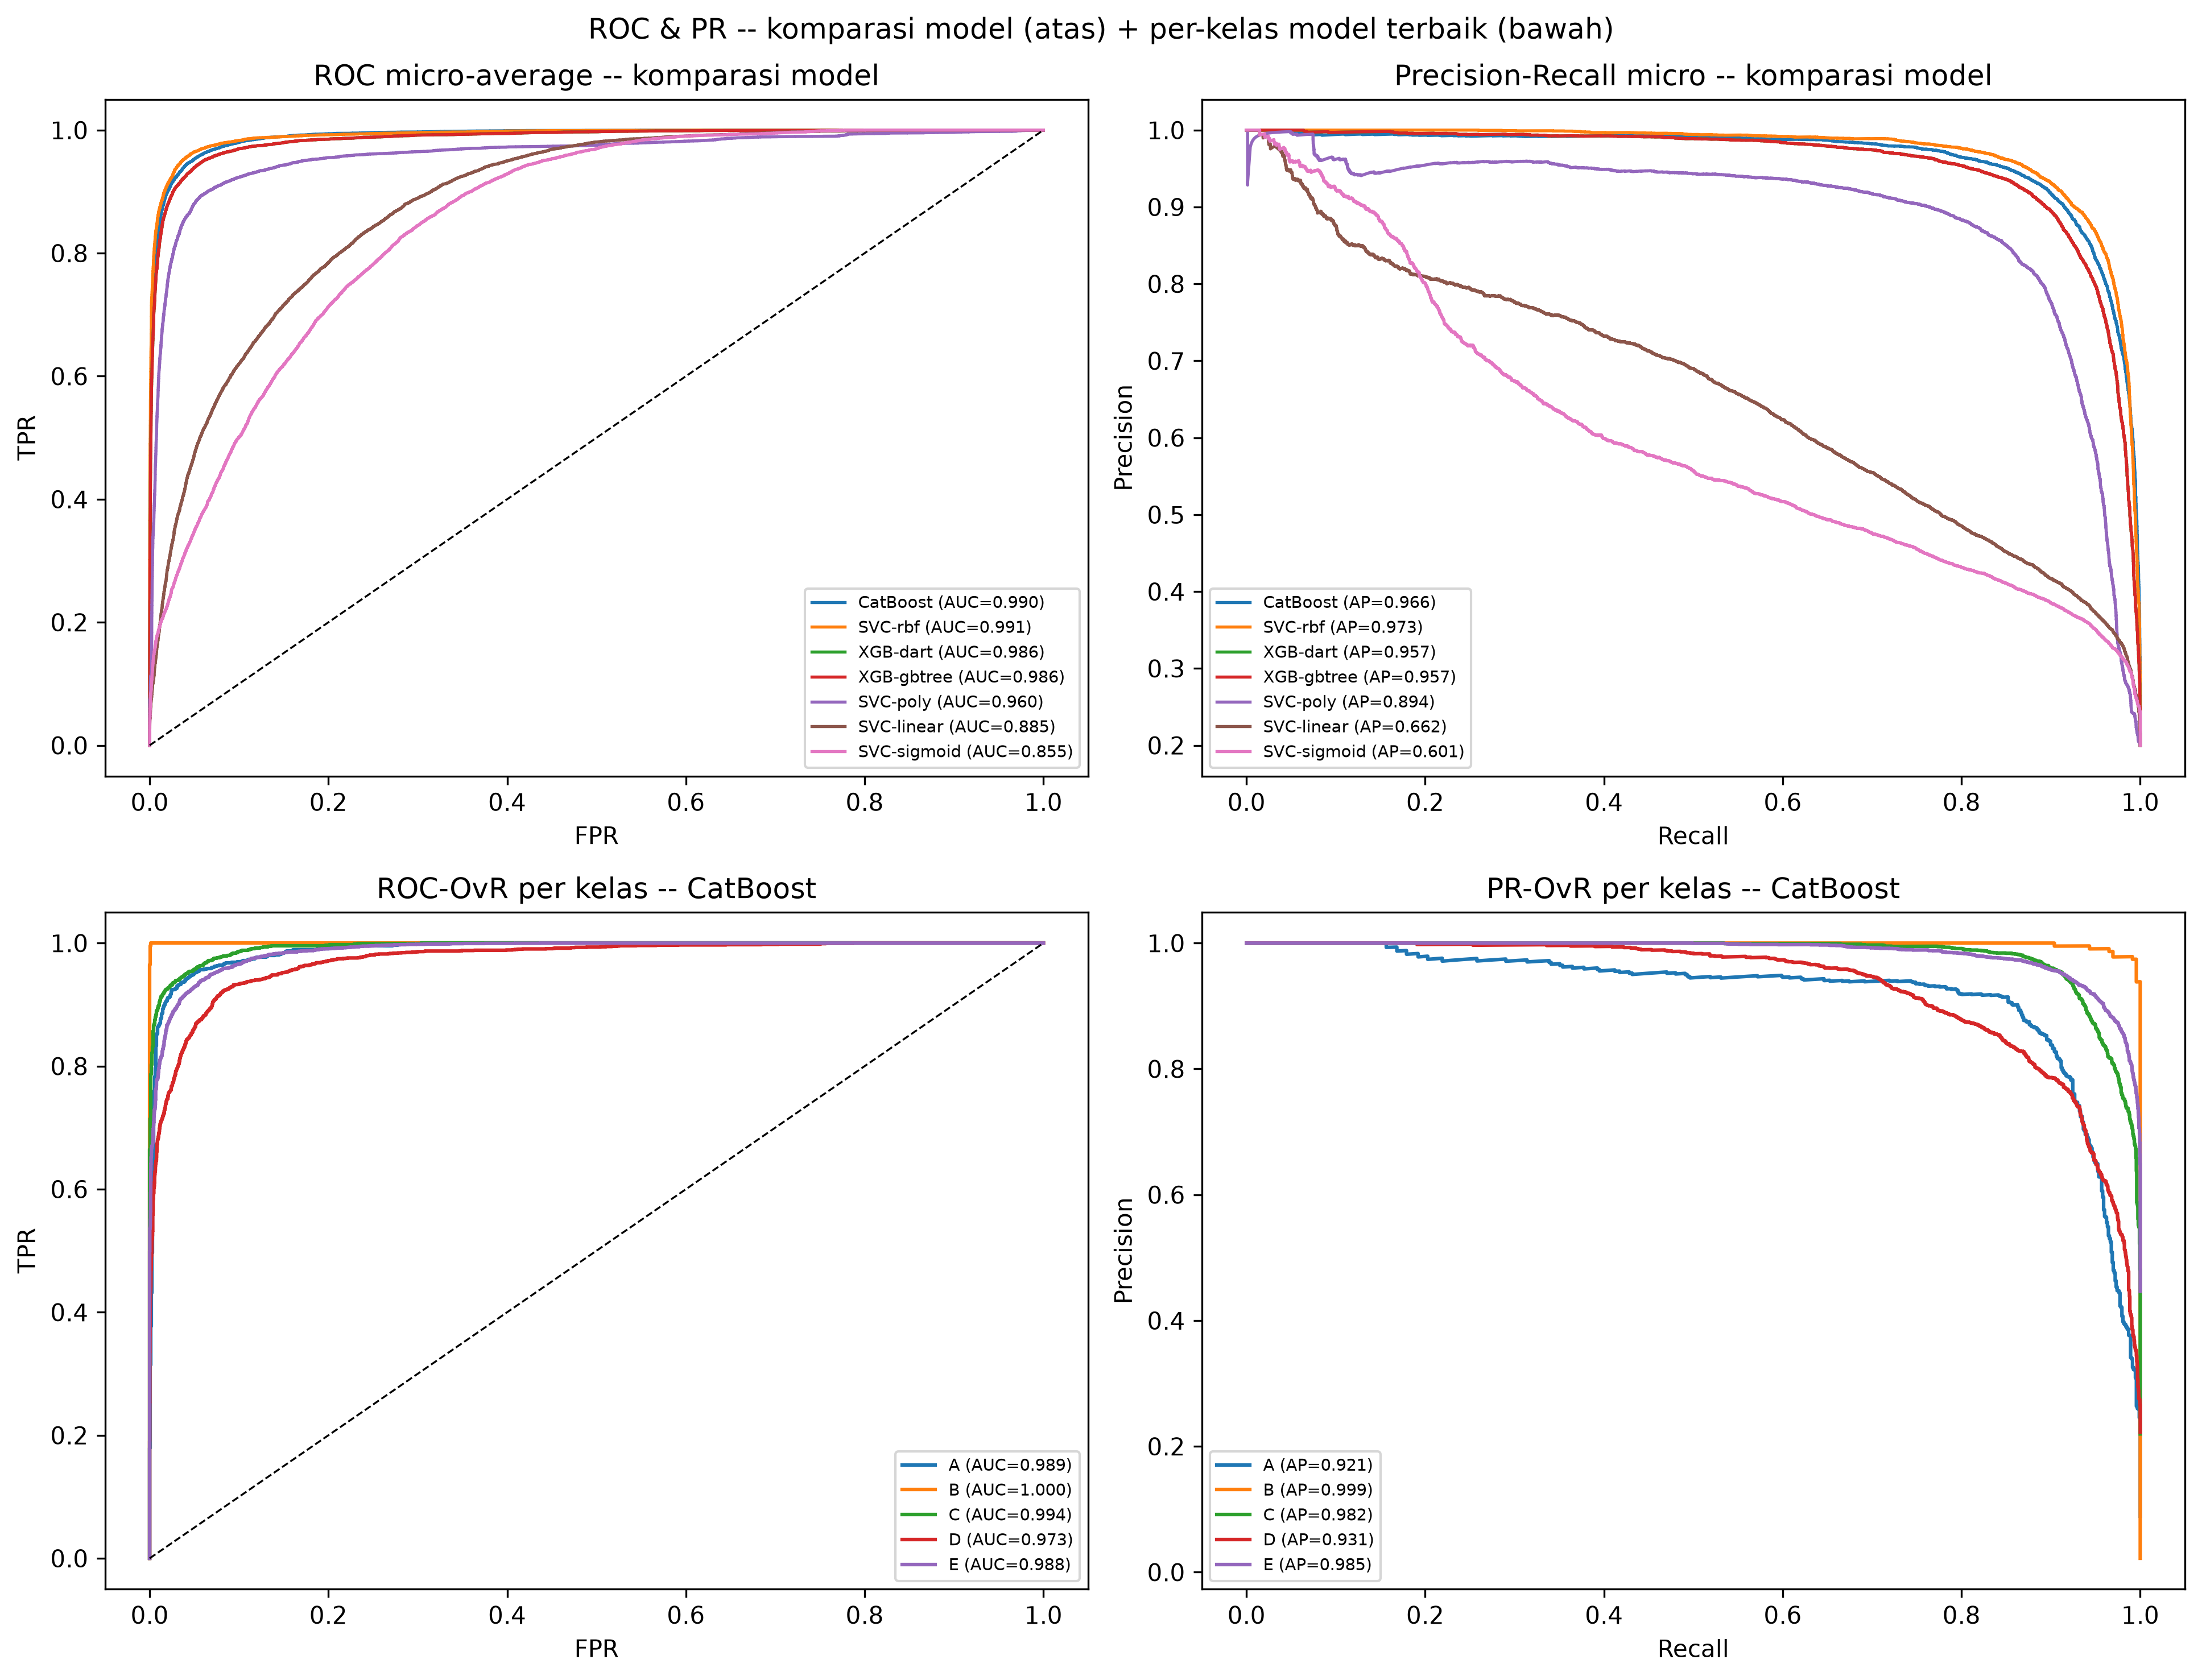
\includegraphics[width=\linewidth]{figure/out-new/12_roc_pr_ovr.png}
\caption{ROC and Precision--Recall curves (one-vs-rest) for the classical models, comparing models (top) and per-class behavior of the best model (bottom).}
\label{fig:classical_roc_pr}
\end{figure}

\begin{figure}[htbp]
\centering

\includegraphics[width=\linewidth]{figure/qml/DL/10_confusion_matrix.png}
\caption{Normalized out-of-fold confusion matrices of the deep learning models (MLP and 1D-CNN), exhibiting the same A--D--E adjacency error pattern.}
\label{fig:dl_confusion}
\end{figure}

\subsection{Model Diagnostic and Limitations}

A diagnostic analysis of the generalization gap is summarized in Fig.~\ref{fig:starv2_gap}. STAR-v2 attains a training macro-F1 of approximately 0.997 and a validation macro-F1 of approximately 0.911, yielding a gap of about 0.086. This gap is not only modest---indicative of mild overfitting---but is also smaller than that of the original \textit{star} map ($\approx 0.107$) and of the tree-based models (whose training F1 reaches 1.0). The finer, bandwidth-scaled encoding of STAR-v2 thus memorizes less while generalizing slightly better. Consistent with the classical analysis, the validation curves are still rising at the full data size and have not plateaued, which implies that the principal bottleneck is the number of \textit{independent} physical samples (only 69 Chop IDs), not model capacity; additional samples would be expected to continue closing the gap.

\begin{figure}[htbp]
\centering

\includegraphics[width=\linewidth]{figure/qml/star-v2/07_gap_train_vs_test_f1.png}
\caption{Train-versus-test macro-F1 gap of STAR-v2, showing milder overfitting than the original \textit{star} map and the tree-based models.}
\label{fig:starv2_gap}
\end{figure}

This pattern is shared across paradigms. For the strong classical tier the train F1 reaches $\approx 1.0$ against a test F1 of $0.89$--$0.91$ (a gap of $0.09$--$0.11$, Fig.~\ref{fig:classical_gap}), and the corresponding learning curves (Fig.~\ref{fig:classical_lc}) are still ascending at the full data size, with the validation log-loss far above the training log-loss---the signature of an overfit limited by data quantity rather than model capacity. By contrast, SVC-linear and SVC-sigmoid show low train and validation F1 alike, the signature of high-bias underfitting. The deep learning models exhibit a nearly identical gap of $0.097$--$0.106$ (Fig.~\ref{fig:dl_gap}) despite EarlyStopping, dropout, $L_2$, and batch normalization, reinforcing that the ceiling is set by the limited number of independent physical samples.

\begin{figure}[htbp]
\centering
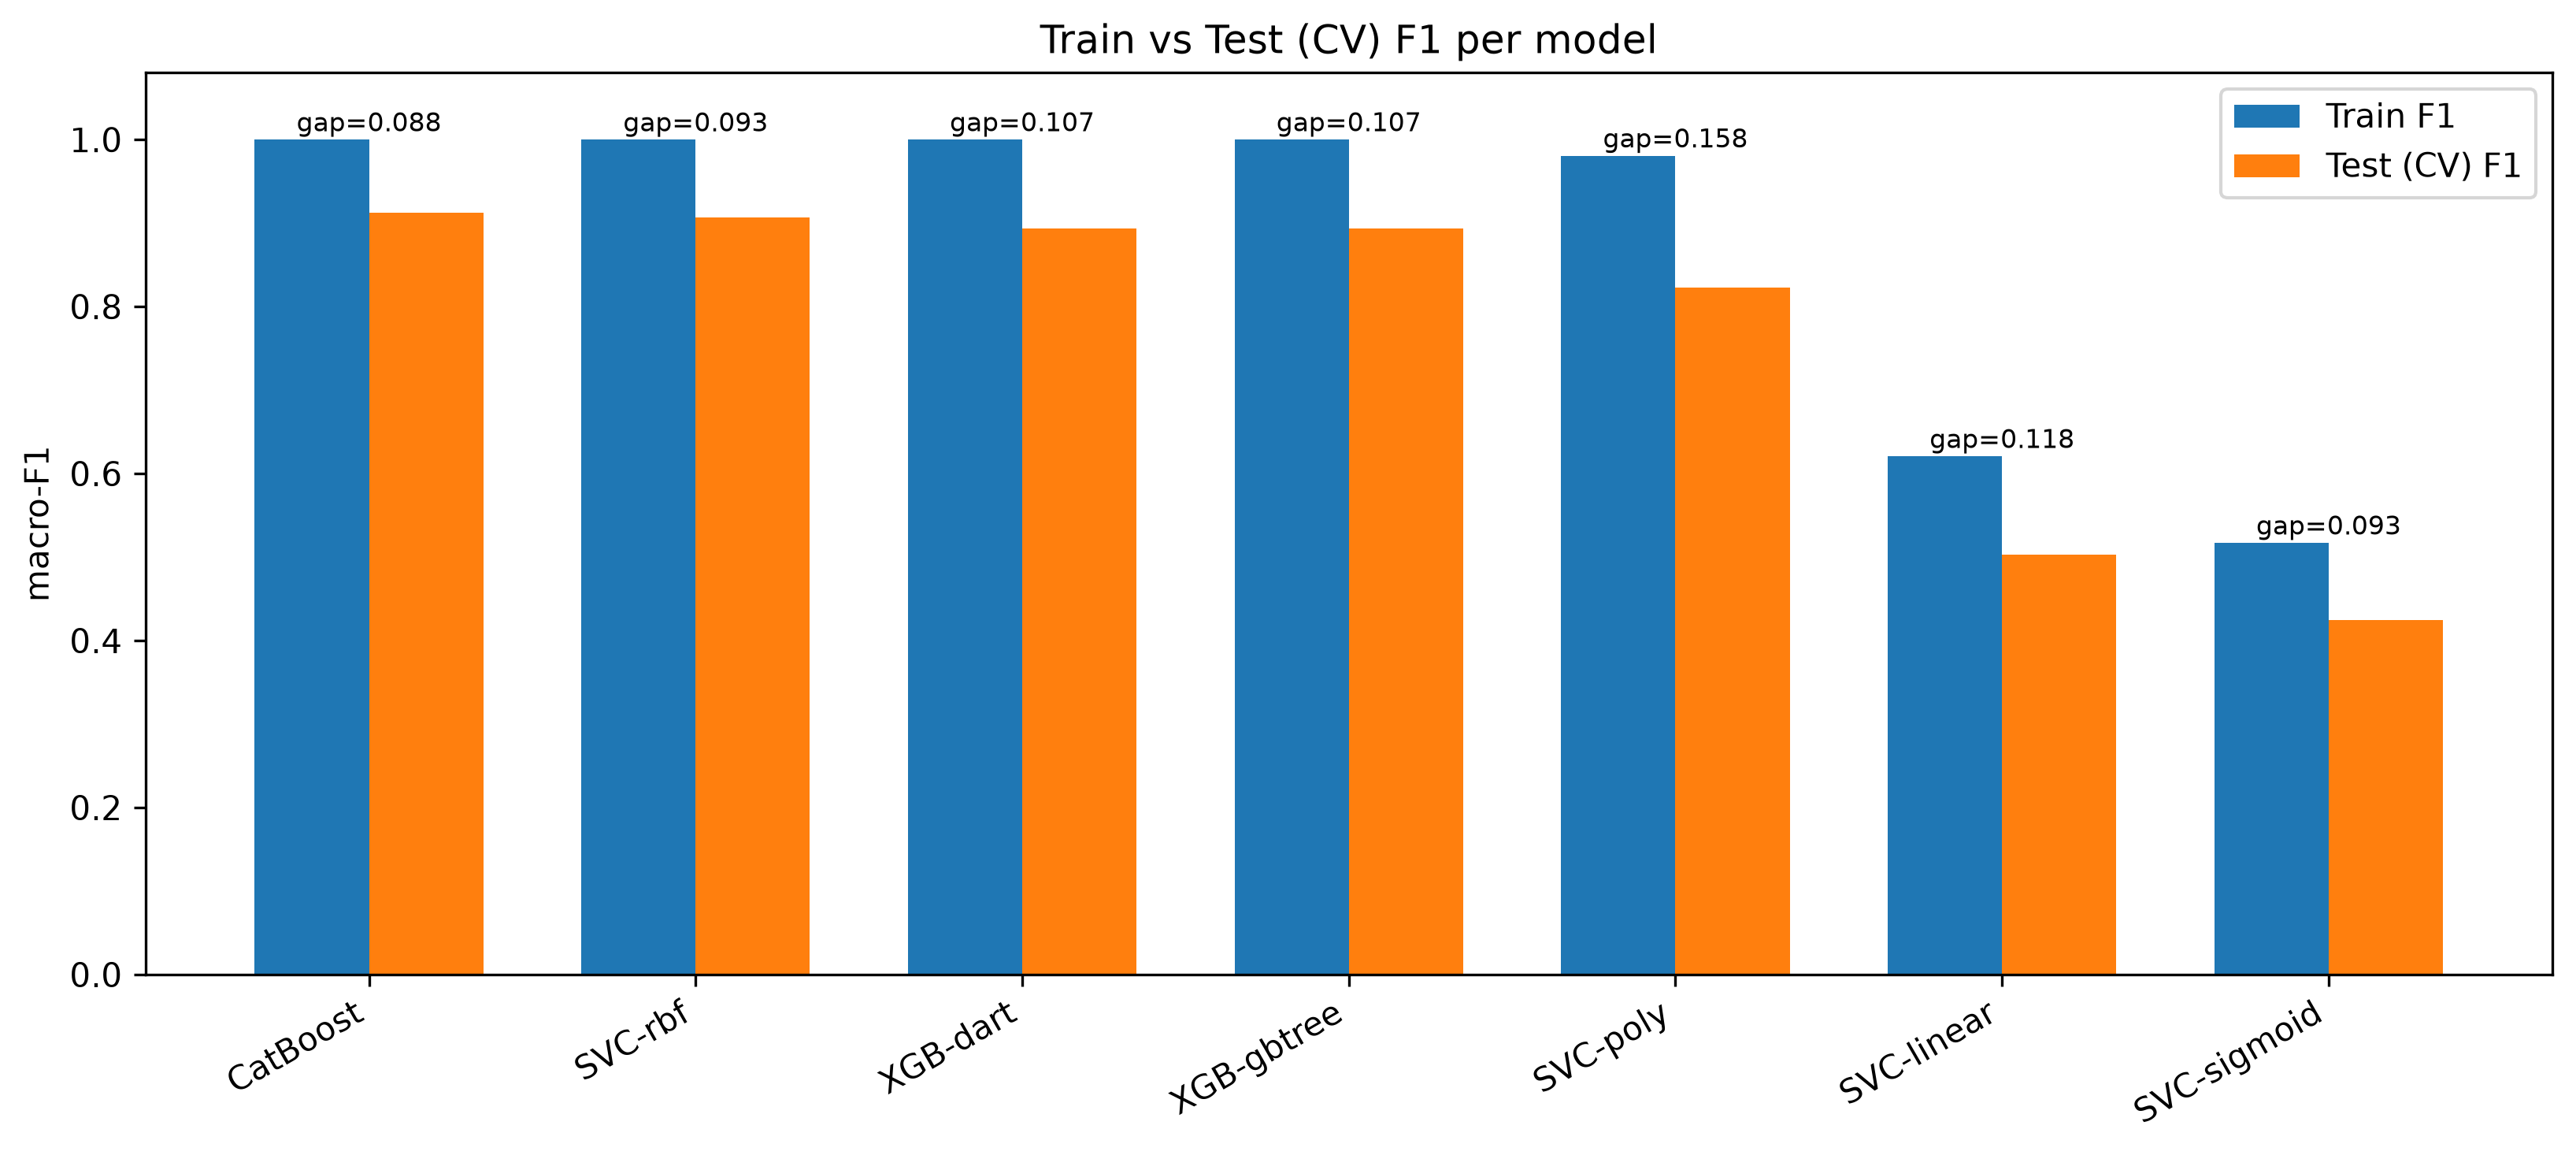
\includegraphics[width=\linewidth]{figure/out-new/07_gap_train_vs_test_f1.png}
\caption{Train-versus-test macro-F1 gap per classical model, separating the mild overfitting of the strong tier from the underfitting of SVC-linear/sigmoid.}
\label{fig:classical_gap}
\end{figure}

\begin{figure}[htbp]
\centering
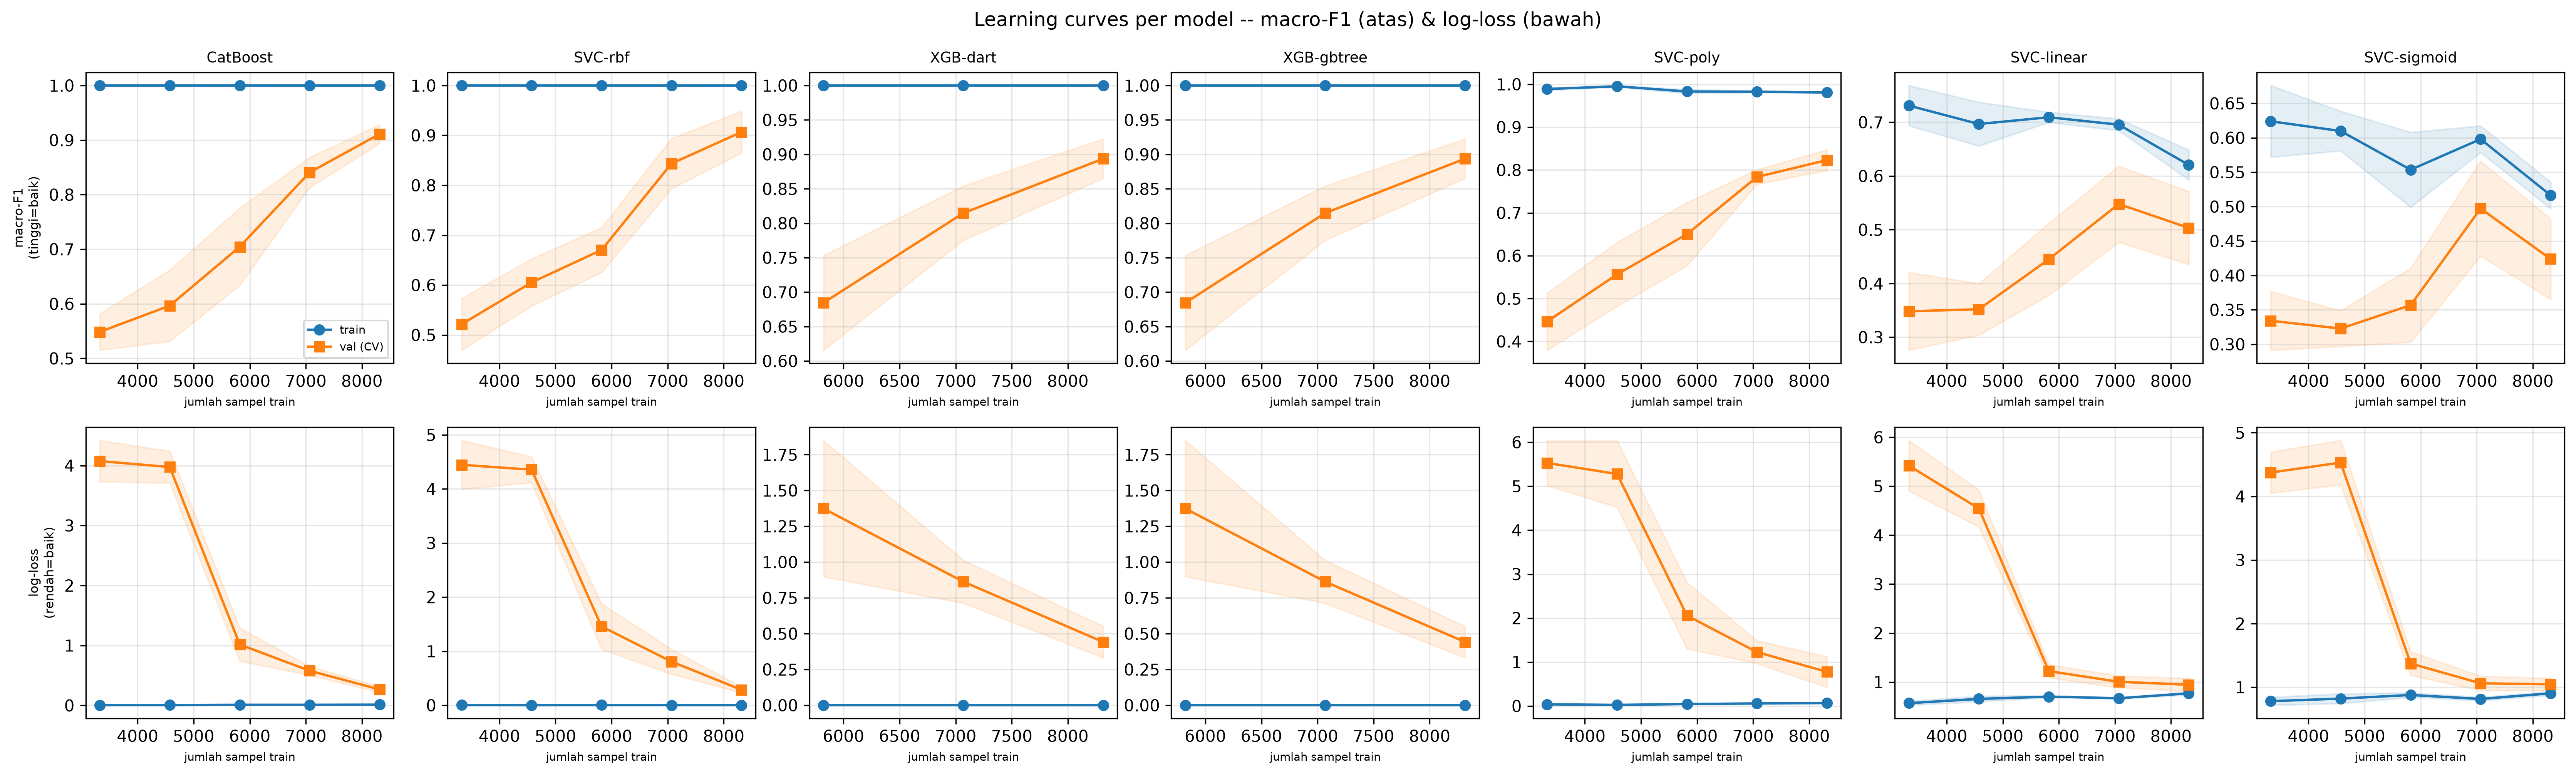
\includegraphics[width=\linewidth]{figure/out-new/09_learning_curve_f1_logloss.png}
\caption{Learning curves (macro-F1, top; log-loss, bottom) for the classical models; the still-rising validation curves indicate the bottleneck is the number of independent samples.}
\label{fig:classical_lc}
\end{figure}

\begin{figure}[htbp]
\centering

\includegraphics[width=\linewidth]{figure/qml/DL/07_gap_train_vs_test_f1.png}
\caption{Train-versus-test macro-F1 gap of the deep learning models, comparable to the strong classical tier and to STAR-v2.}
\label{fig:dl_gap}
\end{figure}

As with the classical models, the probability calibration of STAR-v2 (Fig.~\ref{fig:starv2_calibration}) reveals the common tendency toward overconfidence. While the argmax decisions remain accurate, the raw probability estimates should not be taken at face value; if probabilities or thresholds are to be used in deployment, a calibration step such as temperature scaling or \textit{CalibratedClassifierCV} is recommended.

\begin{figure}[htbp]
\centering

\includegraphics[width=\linewidth]{figure/qml/star-v2/13_calibration.png}
\caption{Reliability diagram for STAR-v2, indicating overconfident probability estimates consistent with the other strong models.}
\label{fig:starv2_calibration}
\end{figure}

The same overconfidence is observed for the classical and deep learning models (Fig.~\ref{fig:classical_calibration} and Fig.~\ref{fig:dl_calibration}), with CatBoost being the closest to ideal calibration. The fold-level stability of STAR-v2 is summarized in Fig.~\ref{fig:starv2_box}, whose tight inter-fold distributions confirm that its top ranking is consistent rather than driven by a single favorable fold.

\begin{figure}[htbp]
\centering
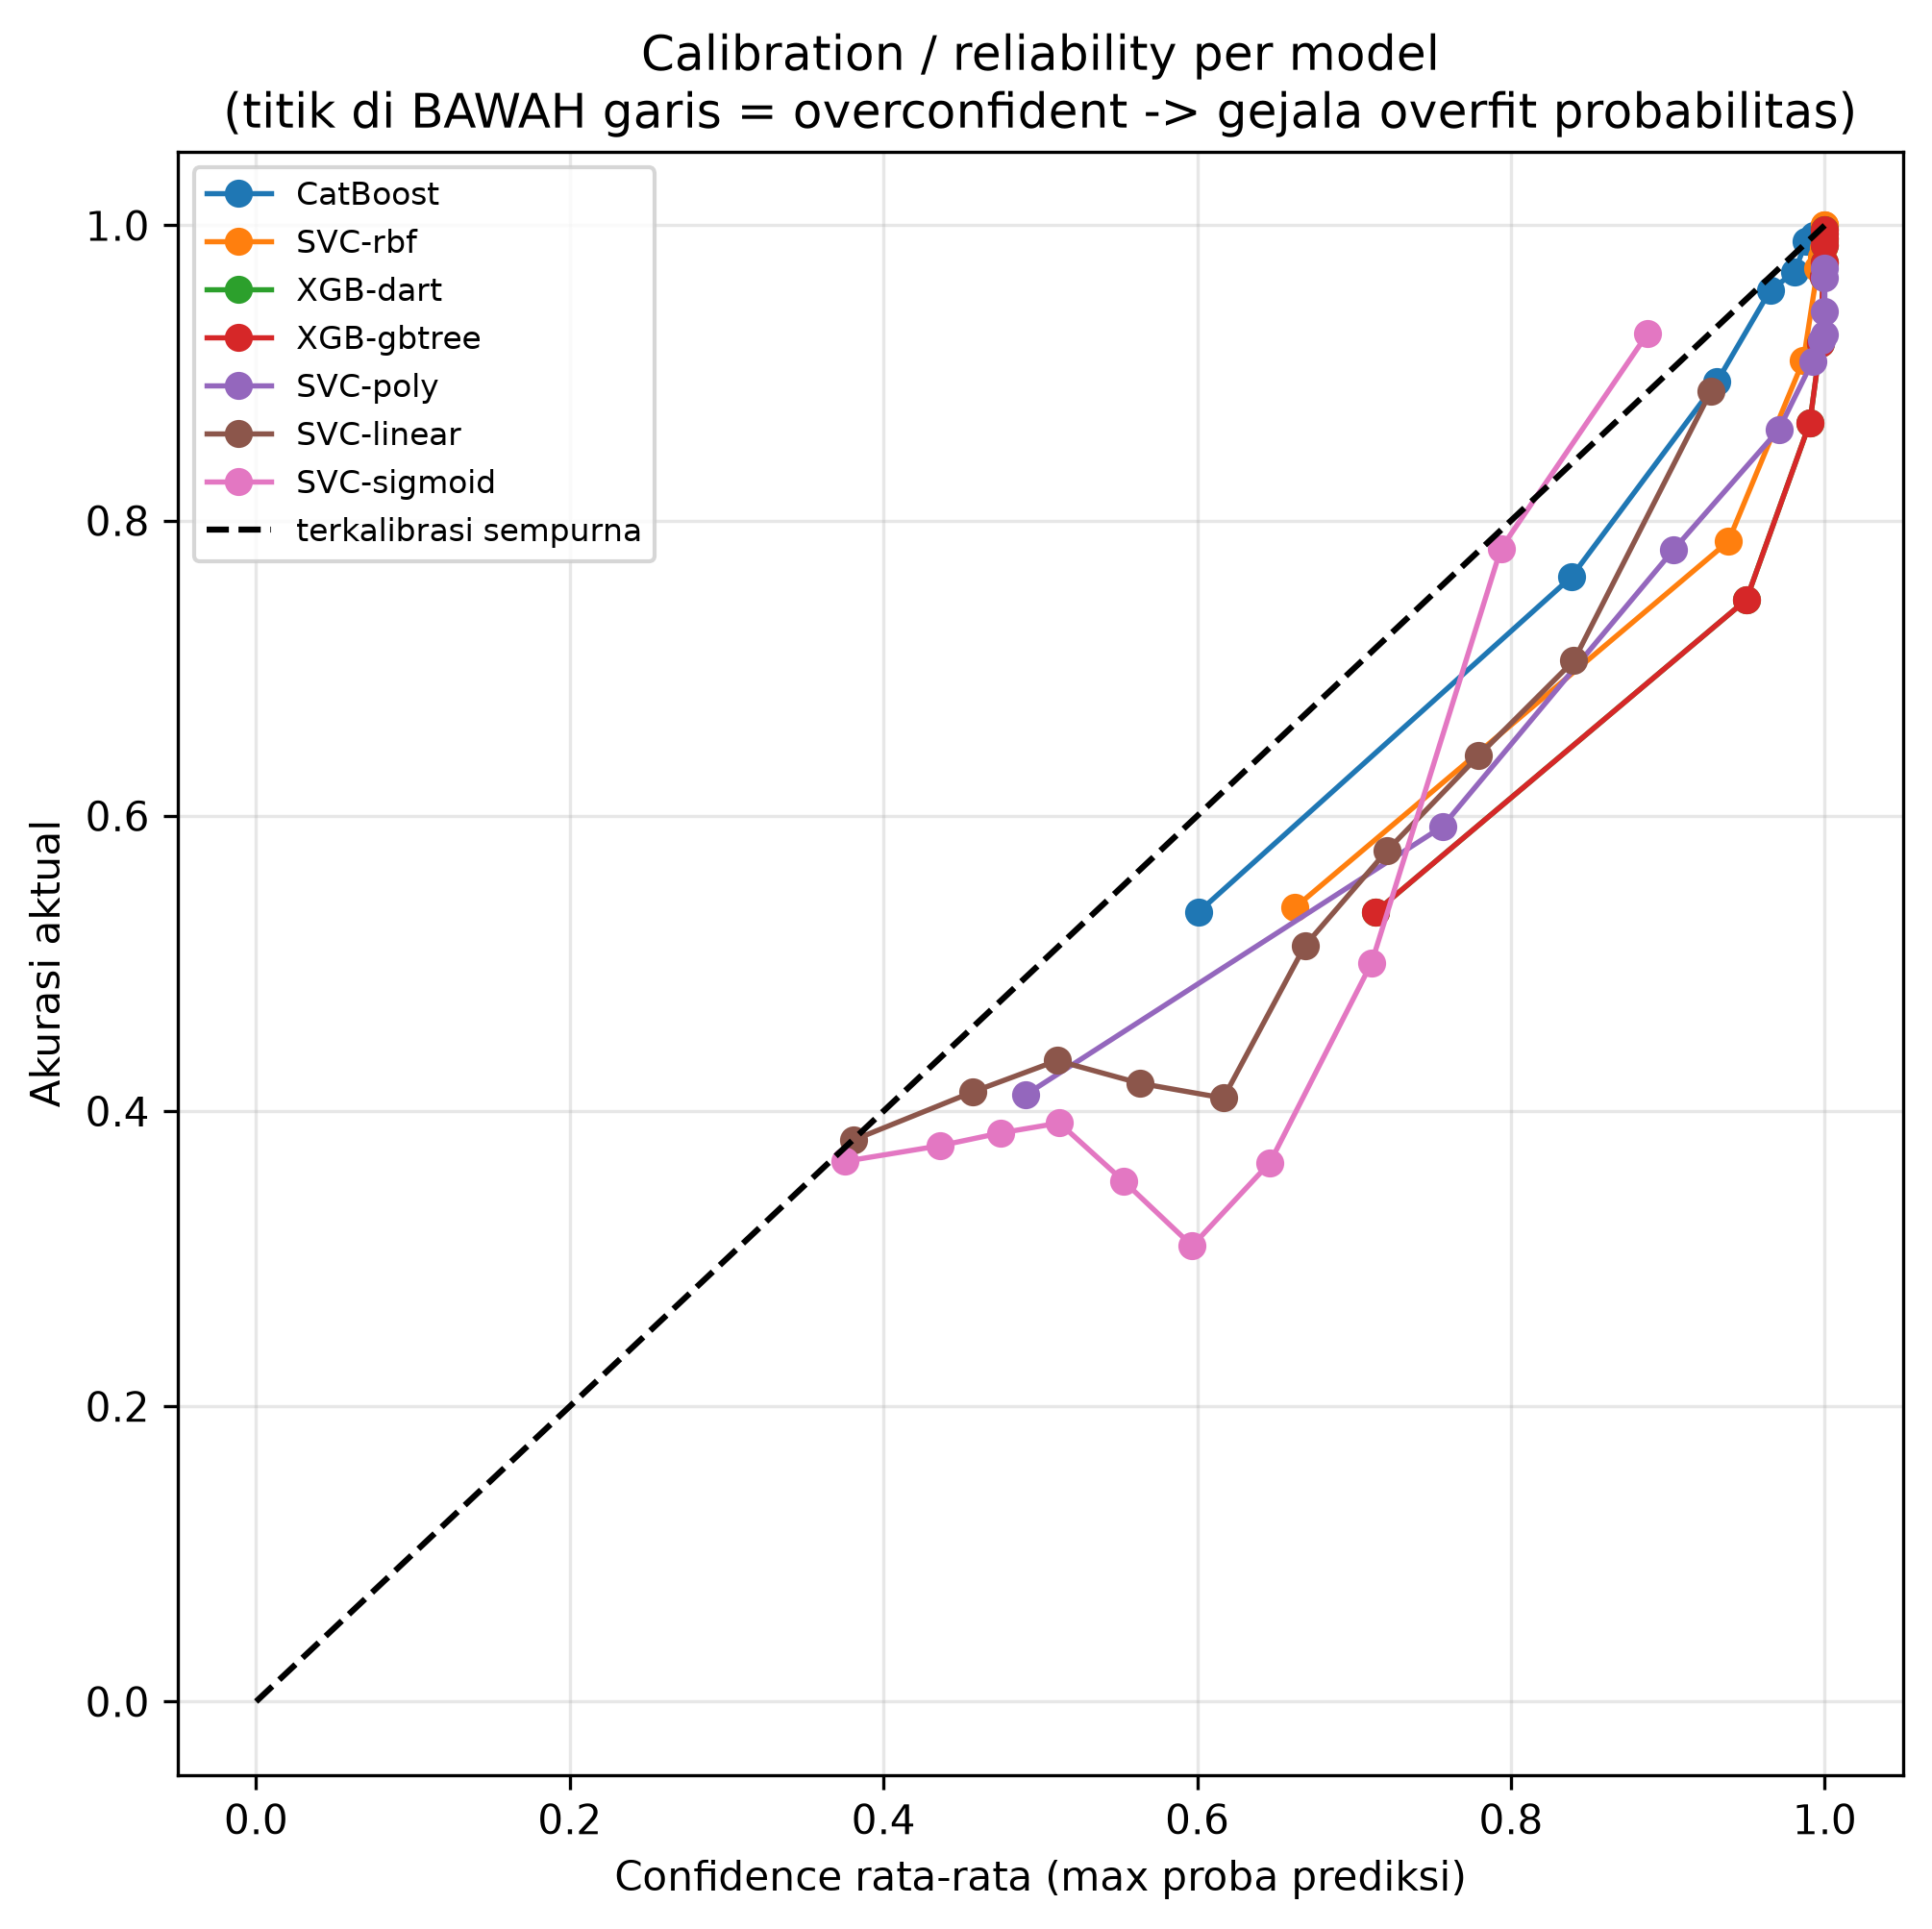
\includegraphics[width=\linewidth]{figure/out-new/13_calibration.png}
\caption{Reliability diagrams of the classical models; all lie below the ideal line (overconfident), with CatBoost the closest to calibrated.}
\label{fig:classical_calibration}
\end{figure}

\begin{figure}[htbp]
\centering

\includegraphics[width=\linewidth]{figure/qml/DL/13_calibration.png}
\caption{Reliability diagrams of the deep learning models, showing the same overconfident tendency as the other strong models.}
\label{fig:dl_calibration}
\end{figure}

\begin{figure}[htbp]
\centering

\includegraphics[width=\linewidth]{figure/qml/star-v2/14_box_perfold_multimetrik.png}
\caption{Per-fold multi-metric distribution of STAR-v2, demonstrating stable performance across the five folds.}
\label{fig:starv2_box}
\end{figure}

Several limitations temper these conclusions and must be stated for honesty. First, the performance differences among the three leading models (0.9379--0.9435) are within the order of the inter-fold standard deviation, so the results should be reported as competitive or marginally favorable to the quantum kernel rather than as an outright quantum dominance. Second, the minority grade B is supported by only two independent physical samples, so the strong B-class figures---observed across all three paradigms---should be regarded as indicative and ideally validated with additional samples. Third, the demonstrated advantage is specific to the kernel/SVM family and to the PRAUC and MCC metrics; there is no blanket quantum advantage across all approaches or metrics on this tabular dataset, which is consistent with the broader literature. Finally, the Composite score is a relative ranking metric whose component zero-points differ, so it must always be read alongside the accompanying raw metrics. Taken together, these caveats frame the principal contribution of this study as an honest and defensible result: a principled, multi-basis quantum feature map (STAR-v2) that renders the quantum kernel competitive with, and marginally superior to, strong classical and deep learning baselines on a real, imbalanced e-nose classification task.

\section{Conclusion}

\begin{thebibliography}{00}

\bibitem{b1} G. O. Young, ``Synthetic structure of industrial plastics,'' in \emph{Plastics,} 2\textsuperscript{nd} ed., vol. 3, J. Peters, Ed. New York, NY, USA: McGraw-Hill, 1964, pp. 15--64.

\bibitem{b2} W.-K. Chen, \emph{Linear Networks and Systems.} Belmont, CA, USA: Wadsworth, 1993, pp. 123--135.

\bibitem{b3} J. U. Duncombe, ``Infrared navigation---Part I: An assessment of feasibility,'' \emph{IEEE Trans. Electron Devices}, vol. ED-11, no. 1, pp. 34--39, Jan. 1959, 10.1109/TED.2016.2628402.

\bibitem{b4} E. P. Wigner, ``Theory of traveling-wave optical laser,'' \emph{Phys. Rev}., vol. 134, pp. A635--A646, Dec. 1965.

\bibitem{b5} E. H. Miller, ``A note on reflector arrays,'' \emph{IEEE Trans. Antennas Propagat}., to be published.

\bibitem{b6} E. E. Reber, R. L. Michell, and C. J. Carter, ``Oxygen absorption in the earth's atmosphere,'' Aerospace Corp., Los Angeles, CA, USA, Tech. Rep. TR-0200 (4230-46)-3, Nov. 1988.

\bibitem{b7} J. H. Davis and J. R. Cogdell, ``Calibration program for the 16-foot antenna,'' Elect. Eng. Res. Lab., Univ. Texas, Austin, TX, USA, Tech. Memo. NGL-006-69-3, Nov. 15, 1987.

\bibitem{b8} \emph{Transmission Systems for Communications}, 3\textsuperscript{rd} ed., Western Electric Co., Winston-Salem, NC, USA, 1985, pp. 44--60.

\bibitem{b9} \emph{Motorola Semiconductor Data Manual}, Motorola Semiconductor Products Inc., Phoenix, AZ, USA, 1989.

\bibitem{b10} G. O. Young, ``Synthetic structure of industrial
plastics,'' in Plastics, vol. 3, Polymers of Hexadromicon, J. Peters,
Ed., 2\textsuperscript{nd} ed. New York, NY, USA: McGraw-Hill, 1964, pp. 15-64.
[Online]. Available:
\underline{http://www.bookref.com}.

\bibitem{b11} \emph{The Founders' Constitution}, Philip B. Kurland
and Ralph Lerner, eds., Chicago, IL, USA: Univ. Chicago Press, 1987.
[Online]. Available: \underline{http://press-pubs.uchicago.edu/founders/}

\bibitem{b12} The Terahertz Wave eBook. ZOmega Terahertz Corp., 2014.
[Online]. Available:
\underline{http://dl.z-thz.com/eBook/zomegaebookpdf\_1206\_sr.pdf}. Accessed on: May 19, 2014.

\bibitem{b13} Philip B. Kurland and Ralph Lerner, eds., \emph{The
Founders' Constitution.} Chicago, IL, USA: Univ. of Chicago Press,
1987, Accessed on: Feb. 28, 2010, [Online] Available:
\underline{http://press-pubs.uchicago.edu/founders/}

\bibitem{b14} J. S. Turner, ``New directions in communications,'' \emph{IEEE J. Sel. Areas Commun}., vol. 13, no. 1, pp. 11-23, Jan. 1995.

\bibitem{b15} W. P. Risk, G. S. Kino, and H. J. Shaw, ``Fiber-optic frequency shifter using a surface acoustic wave incident at an oblique angle,'' \emph{Opt. Lett.}, vol. 11, no. 2, pp. 115--117, Feb. 1986.

\bibitem{b16} P. Kopyt \emph{et al., ``}Electric properties of graphene-based conductive layers from DC up to terahertz range,'' \emph{IEEE THz Sci. Technol.,} to be published. DOI: 10.1109/TTHZ.2016.2544142.

\bibitem{b17} PROCESS Corporation, Boston, MA, USA. Intranets:
Internet technologies deployed behind the firewall for corporate
productivity. Presented at INET96 Annual Meeting. [Online].
Available: \underline{http://home.process.com/Intranets/wp2.htp}

\bibitem{b18} R. J. Hijmans and J. van Etten, ``Raster: Geographic analysis and modeling with raster data,'' R Package Version 2.0-12, Jan. 12, 2012. [Online]. Available: \underline {http://CRAN.R-project.org/package=raster}

\bibitem{b19} Teralyzer. Lytera UG, Kirchhain, Germany [Online].
Available:
\underline{http://www.lytera.de/Terahertz\_THz\_Spectroscopy.php?id=home}, Accessed on: Jun. 5, 2014.

\bibitem{b20} U.S. House. 102\textsuperscript{nd} Congress, 1\textsuperscript{st} Session. (1991, Jan. 11). \emph{H. Con. Res. 1, Sense of the Congress on Approval of}  \emph{Military Action}. [Online]. Available: LEXIS Library: GENFED File: BILLS

\bibitem{b21} Musical toothbrush with mirror, by L.M.R. Brooks. (1992, May 19). Patent D 326 189 [Online]. Available: NEXIS Library: LEXPAT File: DES

\bibitem{b22} D. B. Payne and J. R. Stern, ``Wavelength-switched pas- sively coupled single-mode optical network,'' in \emph{Proc. IOOC-ECOC,} Boston, MA, USA, 1985, pp. 585--590.

\bibitem{b23} D. Ebehard and E. Voges, ``Digital single sideband detection for interferometric sensors,'' presented at the \emph{2\textsuperscript{nd} Int. Conf. Optical Fiber Sensors,} Stuttgart, Germany, Jan. 2-5, 1984.

\bibitem{b24} G. Brandli and M. Dick, ``Alternating current fed power supply,'' U.S. Patent 4 084 217, Nov. 4, 1978.

\bibitem{b25} J. O. Williams, ``Narrow-band analyzer,'' Ph.D. dissertation, Dept. Elect. Eng., Harvard Univ., Cambridge, MA, USA, 1993.

\bibitem{b26} N. Kawasaki, ``Parametric study of thermal and chemical nonequilibrium nozzle flow,'' M.S. thesis, Dept. Electron. Eng., Osaka Univ., Osaka, Japan, 1993.

\bibitem{b27} A. Harrison, private communication, May 1995.

\bibitem{b28} B. Smith, ``An approach to graphs of linear forms,'' unpublished.

\bibitem{b29} A. Brahms, ``Representation error for real numbers in binary computer arithmetic,'' IEEE Computer Group Repository, Paper R-67-85.

\bibitem{b30} IEEE Criteria for Class IE Electric Systems, IEEE Standard 308, 1969.

\bibitem{b31} Letter Symbols for Quantities, ANSI Standard Y10.5-1968.

\bibitem{b32} R. Fardel, M. Nagel, F. Nuesch, T. Lippert, and A. Wokaun, ``Fabrication of organic light emitting diode pixels by laser-assisted forward transfer,'' \emph{Appl. Phys. Lett.}, vol. 91, no. 6, Aug. 2007, Art. no. 061103.~

\bibitem{b33} J. Zhang and N. Tansu, ``Optical gain and laser characteristics of InGaN quantum wells on ternary InGaN substrates,'' \emph{IEEE Photon. J.}, vol. 5, no. 2, Apr. 2013, Art. no. 2600111

\bibitem{b34} S. Azodolmolky~\emph{et al.}, Experimental demonstration of an impairment aware network planning and operation tool for transparent/translucent optical networks,''~\emph{J. Lightw. Technol.}, vol. 29, no. 4, pp. 439--448, Sep. 2011.

\end{thebibliography}

\begin{IEEEbiography}[{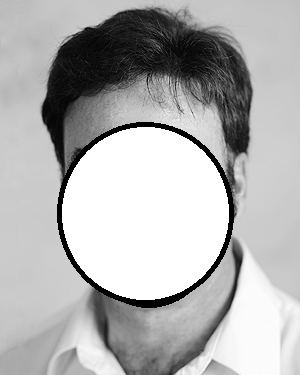
\includegraphics[width=1in,height=1.25in,clip,keepaspectratio]{author1.png}}]{First A. Author} received the B.S. and M.S. degrees in aerospace engineering from
the University of Virginia, Charlottesville, in 2001 and the Ph.D. degree in
mechanical engineering from Drexel University, Philadelphia, PA, in 2008.

From 2001 to 2004, he was a Research Assistant with the Princeton Plasma
Physics Laboratory. Since 2009, he has been an Assistant Professor with the
Mechanical Engineering Department, Texas A{\&}M University, College Station.
He is the author of three books, more than 150 articles, and more than 70
inventions. His research interests include high-pressure and high-density
nonthermal plasma discharge processes and applications, microscale plasma
discharges, discharges in liquids, spectroscopic diagnostics, plasma
propulsion, and innovation plasma applications. He is an Associate Editor of
the journal \emph{Earth, Moon, Planets}, and holds two patents.

Dr. Author was a recipient of the International Association of Geomagnetism
and Aeronomy Young Scientist Award for Excellence in 2008, and the IEEE
Electromagnetic Compatibility Society Best Symposium Paper Award in 2011.
\end{IEEEbiography}


\begin{IEEEbiography}[{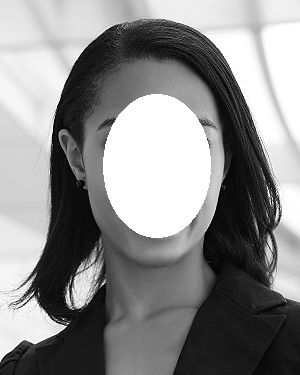
\includegraphics[width=1in,height=1.25in,clip,keepaspectratio]{author2.png}}]{Second B. Author} (M'76--SM'81--F'87) and all authors may include
biographies. Biographies are often not included in conference-related
papers. This author became a Member (M) of IEEE in 1976, a Senior
Member (SM) in 1981, and a Fellow (F) in 1987. The first paragraph may
contain a place and/or date of birth (list place, then date). Next,
the author's educational background is listed. The degrees should be
listed with type of degree in what field, which institution, city,
state, and country, and year the degree was earned. The author's major
field of study should be lower-cased.

The second paragraph uses the pronoun of the person (he or she) and not the
author's last name. It lists military and work experience, including summer
and fellowship jobs. Job titles are capitalized. The current job must have a
location; previous positions may be listed
without one. Information concerning previous publications may be included.
Try not to list more than three books or published articles. The format for
listing publishers of a book within the biography is: title of book
(publisher name, year) similar to a reference. Current and previous research
interests end the paragraph.

The third paragraph begins with the author's
title and last name (e.g., Dr.\ Smith, Prof.\ Jones, Mr.\ Kajor, Ms.\ Hunter).
List any memberships in professional societies other than the IEEE. Finally,
list any awards and work for IEEE committees and publications. If a
photograph is provided, it should be of good quality, and
professional-looking. Following are two examples of an author's biography.
\end{IEEEbiography}

\newpage

%If you do not have or do not want to include a photo, you can use IEEEbiographynophoto as shown below:

\begin{IEEEbiographynophoto}{Third C. Author, Jr.} (M'87) received the B.S. degree in mechanical
engineering from National Chung Cheng University, Chiayi, Taiwan, in 2004
and the M.S. degree in mechanical engineering from National Tsing Hua
University, Hsinchu, Taiwan, in 2006. He is currently pursuing the Ph.D.
degree in mechanical engineering at Texas A{\&}M University, College
Station, TX, USA.

From 2008 to 2009, he was a Research Assistant with the Institute of
Physics, Academia Sinica, Tapei, Taiwan. His research interest includes the
development of surface processing and biological/medical treatment
techniques using nonthermal atmospheric pressure plasmas, fundamental study
of plasma sources, and fabrication of micro- or nanostructured surfaces.

Mr. Author's awards and honors include the Frew Fellowship (Australian
Academy of Science), the I. I. Rabi Prize (APS), the European Frequency and
Time Forum Award, the Carl Zeiss Research Award, the William F. Meggers
Award and the Adolph Lomb Medal (OSA).
\end{IEEEbiographynophoto}

\EOD

\end{document}
